% Capitolul 10: Ipoteza Pieței Fractale (FMH)
% Statistica Piețelor Financiare
% Program de licență, Academia de Studii Economice din București

\documentclass[9pt, aspectratio=169, t]{beamer}

\setbeamersize{text margin left=8mm, text margin right=8mm}

%=============================================================================
% TEMĂ ȘI STIL
%=============================================================================
\usetheme{default}

\definecolor{MainBlue}{RGB}{26, 58, 110}
\definecolor{AccentBlue}{RGB}{26, 58, 110}
\definecolor{IDAred}{RGB}{205, 0, 0}
\definecolor{DarkGray}{RGB}{51, 51, 51}
\definecolor{MediumGray}{RGB}{128, 128, 128}
\definecolor{LightGray}{RGB}{248, 248, 248}
\definecolor{VeryLightGray}{RGB}{235, 235, 235}
\definecolor{KeynoteGray}{RGB}{218, 218, 218}
\definecolor{SectionGray}{RGB}{120, 120, 120}
\definecolor{FooterGray}{RGB}{100, 100, 100}
\definecolor{Crimson}{RGB}{220, 53, 69}
\definecolor{Forest}{RGB}{46, 125, 50}
\definecolor{Amber}{RGB}{181, 133, 63}
\definecolor{Orange}{RGB}{230, 126, 34}
\definecolor{Purple}{RGB}{142, 68, 173}

\setbeamertemplate{background}{%
    \begin{tikzpicture}[remember picture, overlay]
        \shade[shading=axis, shading angle=315,
        top color=LightGray, bottom color=KeynoteGray]
        (current page.south west) rectangle (current page.north east);
    \end{tikzpicture}%
}
\setbeamercolor{background canvas}{bg=}

\setbeamercolor{palette primary}{bg=MainBlue, fg=white}
\setbeamercolor{palette secondary}{bg=MainBlue!85, fg=white}
\setbeamercolor{palette tertiary}{bg=MainBlue!70, fg=white}
\setbeamercolor{structure}{fg=MainBlue}
\setbeamercolor{title}{fg=IDAred}
\setbeamercolor{frametitle}{fg=IDAred, bg=}
\setbeamercolor{block title}{bg=MainBlue, fg=white}
\setbeamercolor{block body}{bg=VeryLightGray, fg=DarkGray}
\setbeamercolor{block title alerted}{bg=Crimson, fg=white}
\setbeamercolor{block body alerted}{bg=Crimson!8, fg=DarkGray}
\setbeamercolor{block title example}{bg=Forest, fg=white}
\setbeamercolor{block body example}{bg=Forest!8, fg=DarkGray}
\setbeamercolor{item}{fg=MainBlue}

\setbeamercolor{author in head/foot}{fg=FooterGray, bg=}
\setbeamercolor{title in head/foot}{fg=FooterGray, bg=}
\setbeamercolor{date in head/foot}{fg=FooterGray, bg=}
\setbeamercolor{section in head/foot}{fg=FooterGray, bg=}
\setbeamercolor{subsection in head/foot}{fg=FooterGray, bg=}

\setbeamertemplate{itemize item}{\color{MainBlue}$\boxdot$}
\setbeamertemplate{itemize subitem}{\color{MainBlue}$\blacktriangleright$}
\setbeamertemplate{itemize subsubitem}{\color{MainBlue}\tiny$\bullet$}
\setbeamertemplate{itemize/enumerate body begin}{\normalsize}
\setbeamertemplate{itemize/enumerate subbody begin}{\normalsize}

\setlength{\leftmargini}{10pt}
\setlength{\leftmarginii}{10pt}
\makeatletter
\def\@listi{\leftmargin\leftmargini \topsep 0pt \parsep 0pt \itemsep 0pt}
\def\@listii{\leftmargin\leftmarginii \topsep 0pt \parsep 0pt \itemsep 0pt}
\makeatother

\setbeamertemplate{navigation symbols}{}

%=============================================================================
% ANTET
%=============================================================================
\setbeamertemplate{headline}{%
    \vskip10pt%
    \hbox to \paperwidth{%
        \hskip0.5cm%
        {\small\color{FooterGray}\thesection.\ \renewcommand{\hyperlink}[2]{##2}\insertsectionhead}%
        \hfill%
        \showlevel\hspace{4pt}%
        \textcolor{FooterGray}{\small\insertframenumber}%
        \hskip0.5cm%
    }%
    \vskip4pt%
    {\color{\currentlevelcolor}\hrule height 1.5pt}%
    \global\slidelevelnum=0%
    \gdef\currentlevelcolor{FooterGray}%
}

%=============================================================================
% SUBSOL
%=============================================================================
\usepackage{fontawesome5}

\setbeamertemplate{footline}{%
    {\color{FooterGray}\hrule height 0.4pt}%
    \vskip4pt%
    \hbox to \paperwidth{%
        \hskip0.5cm%
        \textcolor{FooterGray}{\small Statistica Piețelor Financiare}%
        \hfill%
        \raisebox{-0.1em}{%
            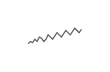
\begin{tikzpicture}[x=0.08em, y=0.08em, line width=0.4pt]
                \draw[FooterGray] (0,3) -- (1,4) -- (2,3.5) -- (3,5) -- (4,4) -- (5,6) -- (6,5.5) -- (7,4) -- (8,5) -- (9,7) -- (10,6) -- (11,5) -- (12,6.5) -- (13,8) -- (14,7) -- (15,6) -- (16,7.5) -- (17,9) -- (18,8) -- (19,7) -- (20,8.5) -- (21,10) -- (22,9) -- (23,8) -- (24,9.5);
            \end{tikzpicture}%
        }%
        \hskip0.5cm%
    }%
    \vskip6pt%
}

%=============================================================================
% PACHETE
%=============================================================================
\usepackage[utf8]{inputenc}
\usepackage[T1]{fontenc}
\usepackage{amsmath, amssymb, amsthm}
\usepackage{mathtools}
\usepackage{bm}
\usepackage{tikz}
\usetikzlibrary{arrows.meta, positioning, shapes, calc, decorations.pathreplacing, shadings}
\usepackage{booktabs}
\usepackage{multirow}
\usepackage{array}
\usepackage{graphicx}
\usepackage{hyperref}
\usepackage{colortbl}
\usepackage{pifont}
\usepackage{listings}
\lstset{language=Python, basicstyle=\ttfamily\scriptsize, keywordstyle=\color{MainBlue}\bfseries,
  commentstyle=\color{Forest}, stringstyle=\color{Crimson}, breaklines=true,
  frame=none, backgroundcolor=\color{VeryLightGray}, xleftmargin=2mm}
\hypersetup{colorlinks=true, linkcolor=MainBlue, urlcolor=MainBlue}
\graphicspath{{../../logos/}{../../charts/}{../../photos/}}
\hfuzz=0.5pt
\vfuzz=0.5pt

%=============================================================================
% COMANDA QUANTLET
%=============================================================================
\newcommand{\quantlet}[2]{%
    \vspace{-0.25cm}%
    \hfill\href{#2}{%
        \raisebox{-0.15em}{
\includegraphics[height=0.7em]{ql_logo.png}}%
        \textcolor{MainBlue}{\tiny\ #1}%
    }\par%
}

% Quantlet inline pentru fiecare figură (centrat, sub imagine)
\newcommand{\figql}[2]{%
    {\centering\href{#2}{%
        \raisebox{-0.15em}{
\includegraphics[height=0.6em]{ql_logo.png}}%
        \textcolor{MainBlue}{\tiny\ #1}%
    }\par}%
}

%=============================================================================
% PAGINĂ TITLU
%=============================================================================
\defbeamertemplate*{title page}{hybrid}[1][]
{
    \vspace{0.2cm}
    \begin{center}
        \href{https://www.ase.ro}{
\includegraphics[height=1.0cm]{ase_logo.png}}\hspace{0.3cm}%
        \href{https://theida.net}{
\includegraphics[height=1.0cm]{ida_logo.png}}\hspace{0.3cm}%
        \href{https://blockchain-research-center.com}{
\includegraphics[height=1.0cm]{brc_logo.png}}\hspace{0.3cm}%
        \href{https://www.ai4efin.ase.ro}{
\includegraphics[height=1.0cm]{ai4efin_logo.png}}\hspace{0.3cm}%
        \href{https://ipe.ro/new}{
\includegraphics[height=1.0cm]{acad_logo.png}}\hspace{0.3cm}%
        \href{https://www.digital-finance-msca.com}{
\includegraphics[height=1.0cm]{msca_logo.png}}%
    \end{center}

    \vspace{0.6cm}

    \begin{center}
        \begin{minipage}{0.1\textwidth}
            \centering
            \href{https://quantlet.com}{
\includegraphics[height=1.1cm]{ql_logo.png}}
        \end{minipage}%
        \begin{minipage}{0.78\textwidth}
            \centering
            {\LARGE\bfseries\usebeamercolor[fg]{title}\inserttitle}

            \vspace{0.3cm}

            {\usebeamerfont{subtitle}\usebeamercolor[fg]{title}\insertsubtitle}
        \end{minipage}%
        \begin{minipage}{0.1\textwidth}
            \centering
            \href{https://quantinar.com}{
\includegraphics[height=1.1cm]{qr_logo.png}}
        \end{minipage}
    \end{center}

    \vspace{0.6cm}

    \hspace{0.5cm}\begin{minipage}[t]{0.9\textwidth}
        \usebeamerfont{author}\insertauthor
    \end{minipage}

    \vspace{0.3cm}

    \hspace{0.5cm}\begin{minipage}[t]{0.9\textwidth}
        \raggedright\small\insertinstitute
    \end{minipage}
}

%=============================================================================
% MEDII PENTRU TEOREME
%=============================================================================
\theoremstyle{definition}
\setbeamertemplate{theorems}[numbered]
\newtheorem{defn}{Definiție}
\newtheorem{thm}{Teoremă}
\newtheorem{prop}{Propoziție}
\newtheorem{rmk}{Observație}

\newenvironment{cminipage}[1]{%
    \par\noindent\hfill\begin{minipage}{#1}\ignorespaces
}{%
    \end{minipage}\hfill\null\par
}

%=============================================================================
% COMENZI PERSONALIZATE
%=============================================================================
\newcommand{\E}{\mathbb{E}}
\newcommand{\Var}{\text{Var}}
\newcommand{\Cov}{\text{Cov}}
\newcommand{\Corr}{\text{Corr}}
\newcommand{\R}{\mathbb{R}}
\newcommand{\N}{\mathbb{N}}
\newcommand{\Z}{\mathbb{Z}}
\newcommand{\B}{\mathbf{B}}
\newcommand{\imark}{\textcolor{MainBlue}{\textbullet}}

% Indicatoare nivel academic
\newcount\slidelevelnum
\global\slidelevelnum=0
\makeatletter
\newcommand{\slidelevel}[1]{%
    \global\slidelevelnum=0%
    \def\tmp@SL{#1}\def\tmp@SLy{Y3}\def\tmp@SLm{MSc}\def\tmp@SLp{PhD}%
    \ifx\tmp@SL\tmp@SLy \global\slidelevelnum=1\fi%
    \ifx\tmp@SL\tmp@SLm \global\slidelevelnum=2\fi%
    \ifx\tmp@SL\tmp@SLp \global\slidelevelnum=3\fi%
}
\makeatother
\gdef\currentlevelcolor{FooterGray}
\newcommand{\showlevel}{%
    \ifnum\slidelevelnum=1%
        \colorbox{Forest}{\strut\textcolor{white}{\sffamily\bfseries\fontsize{8}{9}\selectfont Y3}}%
        \gdef\currentlevelcolor{Forest}%
    \fi%
    \ifnum\slidelevelnum=2%
        \colorbox{MainBlue}{\strut\textcolor{white}{\sffamily\bfseries\fontsize{8}{9}\selectfont MSc}}%
        \gdef\currentlevelcolor{MainBlue}%
    \fi%
    \ifnum\slidelevelnum=3%
        \colorbox{Crimson}{\strut\textcolor{white}{\sffamily\bfseries\fontsize{8}{9}\selectfont PhD}}%
        \gdef\currentlevelcolor{Crimson}%
    \fi%
    \ifnum\slidelevelnum=0%
        \gdef\currentlevelcolor{FooterGray}%
    \fi%
}

%=============================================================================
% INFORMAȚII TITLU
%=============================================================================
\title[Statistica Piețelor Financiare]{Statistica Piețelor Financiare}
\subtitle{Capitolul 10: Ipoteza Pieței Fractale (FMH)}
\author[D.T. Pele, A. Amza]{\texorpdfstring{\begin{tabular}[t]{@{}l@{}}Daniel Traian PELE \\ Antoaneta Amza\end{tabular}}{Daniel Traian PELE, Antoaneta Amza}}
\institute{Academia de Studii Economice din București\\
IDA Institute Digital Assets\\
Blockchain Research Center\\
AI4EFin Artificial Intelligence for Energy Finance\\
Academia Română, Institutul de Prognoză Economică\\
MSCA Digital Finance}
\date{}

\begin{document}

% Pagina de titlu
{
\setbeamertemplate{headline}{}
\setbeamertemplate{footline}{}
\begin{frame}
    \titlepage
\end{frame}
}

%=============================================================================
% OBIECTIVE DE ÎNVĂȚARE
%=============================================================================
\slidelevel{Y3}
\begin{frame}[shrink=15]{Obiective de învățare (Learning Objectives)}
\begin{cminipage}{0.95\textwidth}
\begin{block}{La finalul acestui capitol, veți fi capabili să:}
\begin{enumerate}
    \item[\textcolor{MainBlue}{\textbf{1.}}] \textbf{Identificați} limitele Ipotezei Pieței Eficiente (EMH) și motivele pentru care e nevoie de un cadru fractal
    \item[\textcolor{MainBlue}{\textbf{2.}}] \textbf{Recunoașteți} obiectele fractale (mulțimea Mandelbrot, mulțimi Julia) și fractalii din natură (ferigi, țărmuri, copaci, fulgi de zăpadă)
    \item[\textcolor{MainBlue}{\textbf{3.}}] \textbf{Definiți} autosimilaritatea statistică și dimensiunea fractală (box-counting)
    \item[\textcolor{MainBlue}{\textbf{4.}}] \textbf{Estimați} exponentul Hurst $H$ prin analiza R/S și DFA
    \item[\textcolor{MainBlue}{\textbf{5.}}] \textbf{Interpretați} rezultatele empirice pe acțiuni, cripto, FX (persistent / mers aleator / anti-persistent)
    \item[\textcolor{MainBlue}{\textbf{6.}}] \textbf{Aplicați} mișcarea browniană fracționară (fBm) pentru modelarea memoriei lungi
    \item[\textcolor{MainBlue}{\textbf{7.}}] \textbf{Discutați} multifractalitatea, MMAR și implicațiile pentru managementul riscului
    \item[\textcolor{MainBlue}{\textbf{8.}}] \textbf{Analizați} studii de caz: criza 2008, COVID-19, BVB, Bitcoin
\end{enumerate}
\end{block}
\end{cminipage}
\end{frame}

%=============================================================================
% CUPRINS
%=============================================================================
{
\setbeamertemplate{headline}{%
    \vskip10pt%
    \hbox to \paperwidth{\hskip0.5cm\hfill\hskip0.5cm}%
    \vskip4pt%
    {\color{FooterGray}\hrule height 0.4pt}%
}
\begin{frame}{}
    {\color{FooterGray}\hrule height 0.4pt}
    \vspace{0.1cm}
    {\Large\textcolor{IDAred}{\textbf{Cuprins}}}
    \vspace{0.2cm}
    {\small
    \begin{columns}[T]
        \begin{column}{0.48\textwidth}
            \begin{enumerate}
                \item Motivație: de ce EMH nu este suficientă
                \item Fractali în natură
                \item Autosimilaritate și dimensiune fractală
                \item Mulțimile Mandelbrot și Julia
                \item Exponentul Hurst
                \item Analiza R/S
                \item DFA (Detrended Fluctuation Analysis)
            \end{enumerate}
        \end{column}
        \begin{column}{0.48\textwidth}
            \begin{enumerate}\setcounter{enumi}{7}
                \item Mișcarea browniană fracționară (fBm)
                \item Ipoteza Pieței Fractale (FMH)
                \item Multifractalitate și MMAR
                \item Evidență empirică
                \item Studii de caz reale
                \item Implicații pentru managementul riscului
                \item Concluzii și referințe
            \end{enumerate}
        \end{column}
    \end{columns}
    }
\end{frame}
}

%#############################################################################
\section{Motivație}
%#############################################################################

\slidelevel{Y3}
\begin{frame}[shrink=15]{De ce avem nevoie de o nouă paradigmă?}
\begin{cminipage}{0.95\textwidth}
\begin{columns}[T]
\begin{column}{0.55\textwidth}
\begin{itemize}\setlength{\itemsep}{1pt}
    \item \textbf{Eșecuri empirice ale EMH} (Capitolul 4)
    \begin{itemize}\setlength{\itemsep}{0pt}
        \item \textbf{Cozi grele:} $\Pr(|r_t| > x) \gg \Phi(-x)$ pentru $x$ mare
        \item \textbf{Volatility clustering:} $\Corr(|r_t|, |r_{t+k}|) > 0$
        \item \textbf{Memorie lungă:} $\rho(k) \sim C k^{2H-2}$, $H > 0{,}5$
        \item \textbf{Crah-uri:} 1987 ($-22{,}6\%$), 2008, COVID-2020
    \end{itemize}
    \item \textbf{Sub gaussianitate}, probabilitatea Black Monday 1987
    \[
        \Pr(r \leq -22{,}6\%) \approx 10^{-50} \;\; (\text{practic 0})
    \]
    \item \textbf{Mandelbrot (1963):} prețurile bumbacului prezintă \textit{varianță infinită}
    \item \textbf{Peters (1991, 1994):} propune Ipoteza Pieței Fractale (FMH)
    \begin{itemize}\setlength{\itemsep}{0pt}
        \item Piețele sunt sisteme \textbf{fractale}
        \item Investitorii operează pe \textbf{orizonturi multiple}
        \item Stabilitatea $\Leftrightarrow$ \textbf{diversitatea} orizonturilor
    \end{itemize}
\end{itemize}
\end{column}
\begin{column}{0.42\textwidth}
\centering
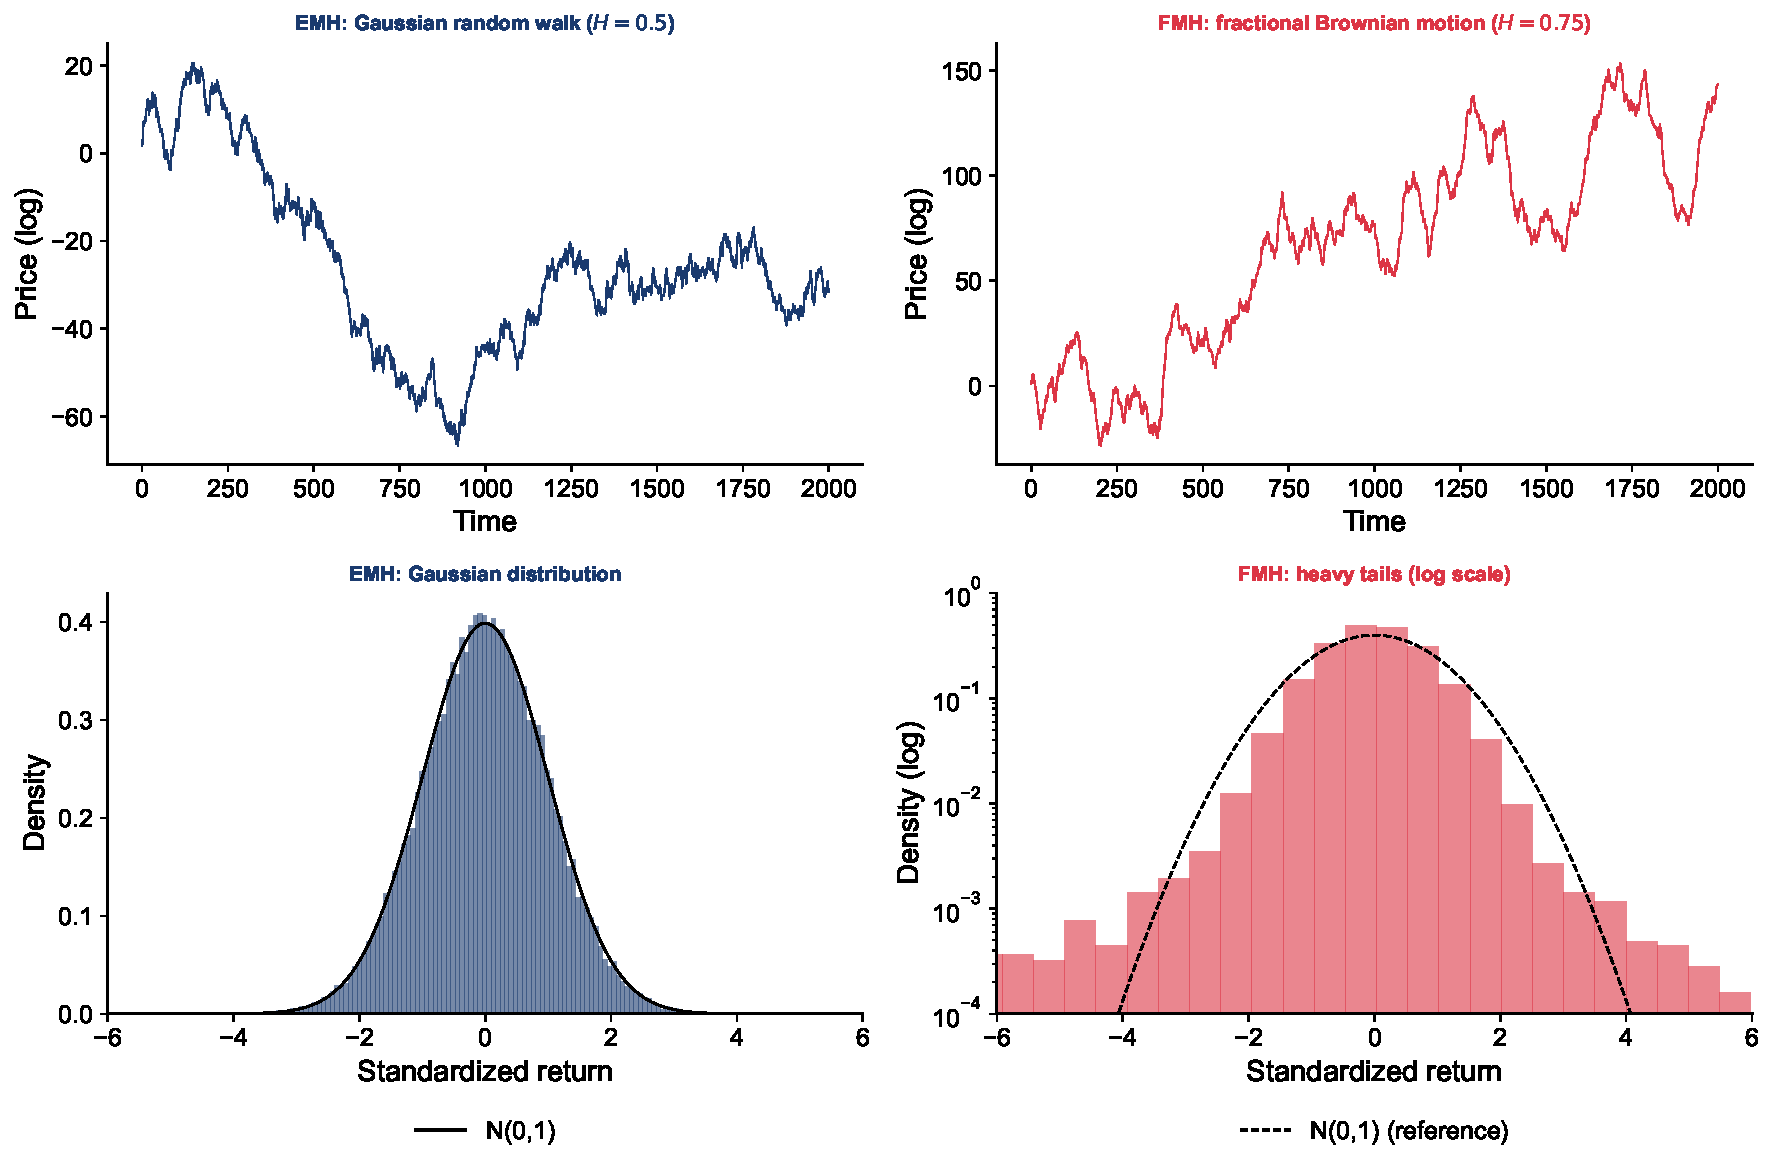
\includegraphics[width=\linewidth]{ch_fmh_emh_vs_fmh.pdf}
{\scriptsize\textcolor{MediumGray}{\textit{Sus: traiectorii de preț EMH (gaussian) vs FMH (fBm $H=0{,}75$). Jos: distribuția randamentelor — coadă subțire (gaussiană) vs coadă grea.}}}
\figql{SFM\_ch\_fmh\_fractals: emh\_vs\_fmh}{https://github.com/QuantLet/Stat_fin_markets/tree/master/Quantlets/SFM_ch_fmh}
\end{column}
\end{columns}
\end{cminipage}
\end{frame}

\slidelevel{Y3}
\begin{frame}[shrink=15]{De la geometria euclidiană la fractali}
\begin{cminipage}{0.95\textwidth}
\begin{columns}[T]
\begin{column}{0.50\textwidth}
\begin{block}{Geometria euclidiană}
\begin{itemize}\setlength{\itemsep}{0pt}
    \item Lume \textbf{netedă}, \textbf{regulată}
    \item Obiecte: drepte, cercuri, sfere
    \item Dimensiuni \textbf{întregi}: $D \in \{0, 1, 2, 3\}$
    \item Adecvată pentru: case, mașini, mecanică clasică
\end{itemize}
\end{block}

\begin{block}{Geometria fractală (Mandelbrot, 1975)}
\begin{itemize}\setlength{\itemsep}{0pt}
    \item Lume \textbf{aspră}, \textbf{neregulată}, \textbf{autosimilară}
    \item Obiecte: țărmuri, nori, copaci, randamente bursiere
    \item Dimensiuni \textbf{fracționare}: $D \in \R$
    \item Adecvată pentru: \textbf{natură} și \textbf{piețe financiare}
\end{itemize}
\end{block}
\end{column}
\begin{column}{0.46\textwidth}
\begin{center}
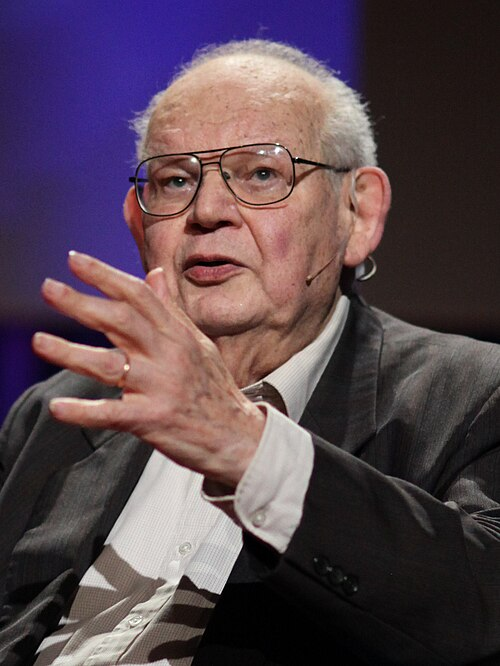
\includegraphics[height=2.6cm,keepaspectratio]{mandelbrot.jpg}\\[1pt]
{\scriptsize\textcolor{MediumGray}{\textbf{Benoît Mandelbrot} (1924--2010)}}
\figql{Wikimedia Commons}{https://en.wikipedia.org/wiki/Benoit_Mandelbrot}
\end{center}
\vspace{0.1cm}
\begin{alertblock}{Citat (Mandelbrot, 1982)}
\begin{itemize}\setlength{\itemsep}{0pt}
    \item \textit{,,Norii nu sunt sfere''}
    \item \textit{,,Munții nu sunt conuri''}
    \item \textit{,,Țărmurile nu sunt cercuri''}
    \item \textit{,,Scoarța nu este netedă''}
    \item \textit{,,Fulgerul nu călătorește în linie dreaptă''}
\end{itemize}
\end{alertblock}
\end{column}
\end{columns}
\end{cminipage}
\end{frame}

\slidelevel{Y3}
\begin{frame}[shrink=15]{Context istoric}
\begin{cminipage}{0.95\textwidth}
\renewcommand{\arraystretch}{1.2}
\begin{center}
\small
\begin{tabular}{lll}
\toprule
\textbf{An} & \textbf{Autor} & \textbf{Contribuție} \\
\midrule
1872 & Karl Weierstrass & Funcție continuă peste tot, nicăieri diferențiabilă \\
1883 & Georg Cantor & Mulțimea Cantor (primul fractal modern) \\
1904 & Helge von Koch & Curba Koch / fulgul de zăpadă \\
1918 & Gaston Julia & Mulțimile Julia (analiza dinamicii complexe) \\
1951 & Harold E. Hurst & Exponentul $H$ (studiul Nilului) \\
1963 & Benoît Mandelbrot & ,,The variation of certain speculative prices'' \\
1975 & Mandelbrot & Termenul \textit{,,fractal''}; mulțimea Mandelbrot \\
1969 & Mandelbrot \& Wallis & Analiza R/S aplicată în finanțe \\
1991 & Edgar Peters & ,,Chaos and Order in the Capital Markets'' \\
1994 & Peng et al. & Detrended Fluctuation Analysis (DFA) \\
1997 & Mandelbrot, Fisher, Calvet & MMAR (Multifractal Model of Asset Returns) \\
2004 & Mandelbrot \& Hudson & ,,The (Mis)Behavior of Markets'' \\
\bottomrule
\end{tabular}
\end{center}
\end{cminipage}
\end{frame}

\slidelevel{Y3}
\begin{frame}[shrink=15]{Anomalii care contrazic EMH (Anomalies contradicting EMH)}
\begin{cminipage}{0.95\textwidth}
\renewcommand{\arraystretch}{1.2}
\begin{center}
\small
\begin{tabular}{lll}
\toprule
\textbf{Anomalie (Anomaly)} & \textbf{Descriere} & \textbf{Predicție EMH} \\
\midrule
Cozi grele (heavy tails) & $\Pr(|r|>5\sigma) \sim 100\times$ Gaussian & Imposibil sub gaussianitate \\
Volatility clustering & $\Corr(r^2_t, r^2_{t-k}) > 0$ pentru $k$ mare & Independență $\Rightarrow$ corelație 0 \\
Memorie lungă (long memory) & $\rho(k) \sim k^{2H-2}$, $H>0{,}5$ & $\rho(k) = 0$ pentru $k > 0$ \\
Efect ianuarie (January effect) & Randamente medii ianuarie $>$ alte luni & Imposibil dacă cunoscut \\
Momentum (3--12 luni) & Câștigătorii continuă să câștige & Imposibil sub mers aleator \\
Reversal (3--5 ani) & Câștigătorii pe termen lung pierd & Imposibil sub independență \\
PEAD (post-earnings drift) & Drift după anunțuri trimestriale & Reflectare instantanee \\
Effect ,,Black Monday'' (1987) & $-22{,}6\%$ într-o zi & Probabilitate $\sim 10^{-50}$ \\
Bule speculative (bubbles) & DotCom 2000, criptoactive 2017 & Excluse de raționalitate \\
\bottomrule
\end{tabular}
\end{center}
\vspace{0.2cm}
\begin{itemize}\setlength{\itemsep}{0pt}
    \item Toate aceste fenomene au în comun: \textbf{auto-similaritate la scale temporale diferite} și \textbf{dependență temporală}
    \item EMH presupune Brownian; FMH propune \textbf{fBm} (mișcare browniană fracționară --- generalizare a Brownianului standard cu memorie reglată de exponentul Hurst $H$; $H = 0{,}5$ recuperează Brownian; definiție formală în §8) și măsuri multifractale
\end{itemize}
\end{cminipage}
\end{frame}

\slidelevel{Y3}
\begin{frame}[shrink=15]{De la mers aleator la fractali (From random walk to fractals)}
\begin{cminipage}{0.95\textwidth}
\begin{columns}[T]
\begin{column}{0.50\textwidth}
\begin{block}{Bachelier (1900): mers aleator (random walk)}
\begin{itemize}\setlength{\itemsep}{0pt}
    \item Variația prețului în $\Delta t$: $\Delta P \sim \mathcal{N}(0, \sigma^2 \Delta t)$
    \item Implicit: $H = 0{,}5$
    \item Formă \textbf{netedă} de variabilitate (smooth)
\end{itemize}
\end{block}

\begin{block}{Mandelbrot (1963, 1967): randomness fractal}
\begin{itemize}\setlength{\itemsep}{0pt}
    \item Dimensiune fractală reală a graficului preț: $D = 2 - H \neq 1{,}5$
    \item Cu cât $D$ e mai mare, cu atât graficul e mai \textbf{neregulat}
    \item Indici reali: $D \in [1{,}3;\, 1{,}5]$ $\Rightarrow$ \textbf{nu} mers aleator pur
\end{itemize}
\end{block}
\end{column}
\begin{column}{0.46\textwidth}
\centering
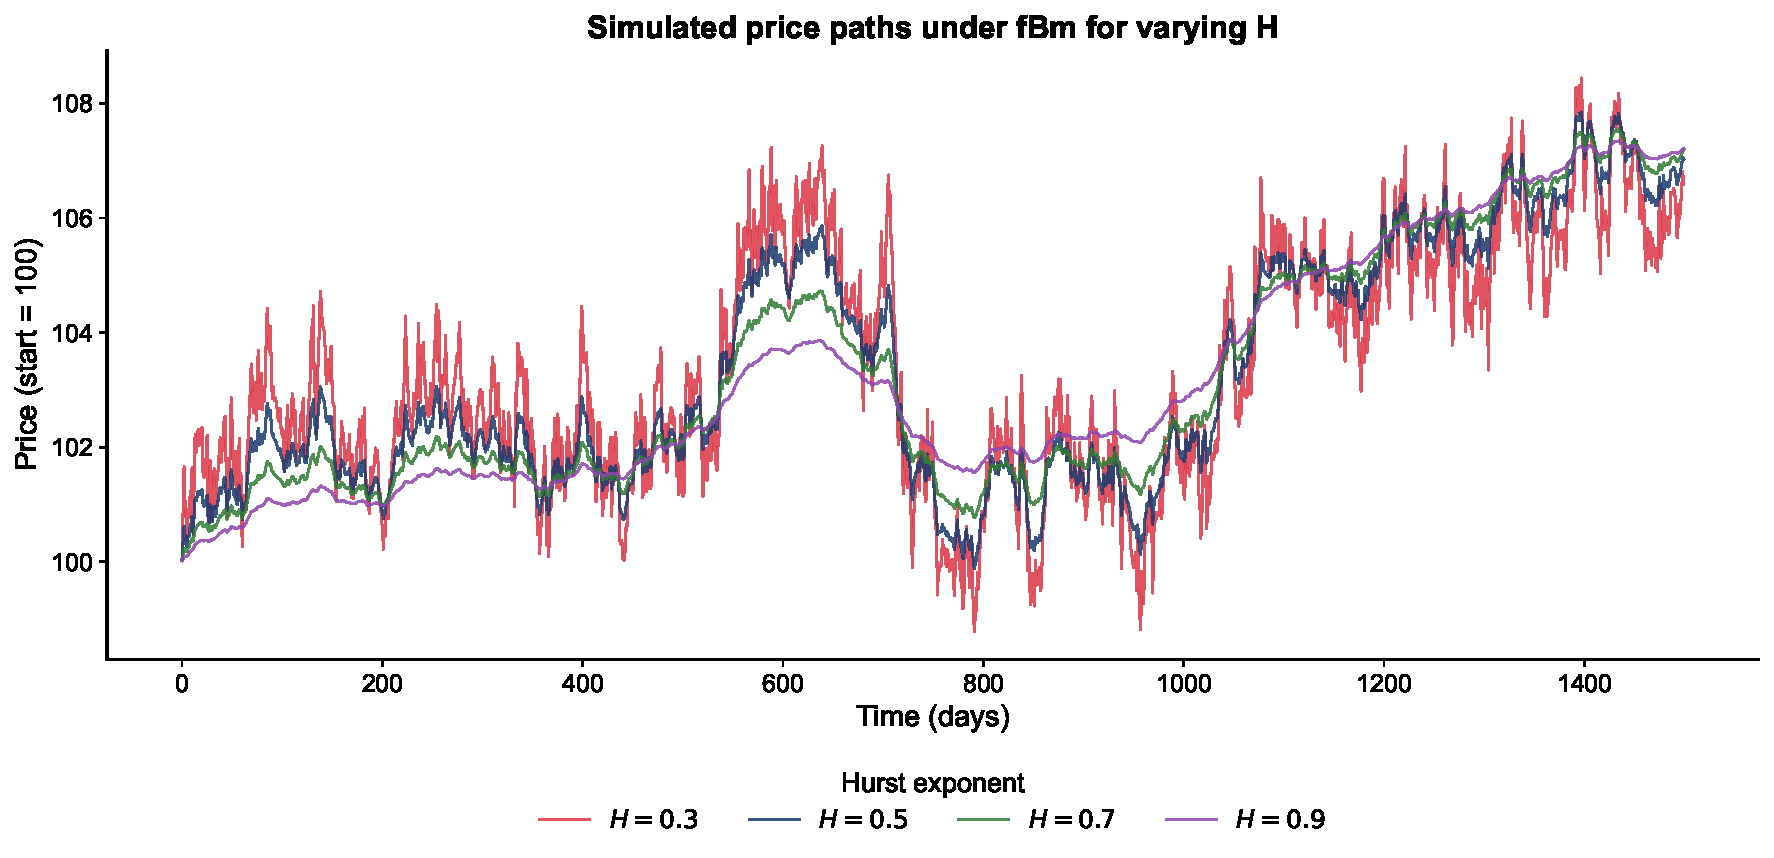
\includegraphics[width=\linewidth,height=4.6cm,keepaspectratio]{ch_fmh_price_paths_H.pdf}\\[2pt]
{\scriptsize\textcolor{MediumGray}{\textit{Traiectorii de preț simulate pentru patru valori ale exponentului Hurst $H$.}}}
\figql{SFM\_ch\_fmh\_extra: price\_paths\_H}{https://github.com/QuantLet/Stat_fin_markets/tree/master/Quantlets/SFM_ch_fmh}
\end{column}
\end{columns}
\end{cminipage}
\end{frame}

\slidelevel{MSc}
\begin{frame}[shrink=15]{Întrebări fundamentale (Open questions in finance)}
\begin{cminipage}{0.95\textwidth}
\begin{itemize}\setlength{\itemsep}{1pt}
    \item \textbf{Q1.} Sunt randamentele bursiere \textbf{i.i.d.}? \\
    EMH: Da. \textbf{Evidența empirică}: Nu (vezi cozi grele, vol. clustering)
    \item \textbf{Q2.} Există \textbf{memorie pe termen lung} (long-range dependence)? \\
    EMH: Nu, $\rho(k) = 0$. \textbf{Evidența empirică}: Da (Hurst $> 0{,}5$ pentru majoritatea acțiunilor)
    \item \textbf{Q3.} Crah-urile sunt \textbf{,,lebede negre''} (black swans, Taleb 2007) sau \textbf{eșecuri structurale}? \\
    EMH: Lebede negre. \textbf{FMH}: Eșecuri structurale (collapse of horizons)
    \item \textbf{Q4.} Volatilitatea scalează cu $\sqrt{T}$ sau cu $T^H$? \\
    EMH: $\sqrt{T}$. \textbf{Evidența}: $T^H$ cu $H \in [0{,}55;\, 0{,}65]$
    \item \textbf{Q5.} Există \textbf{auto-similaritate} (self-similarity) între scale temporale? \\
    EMH: Aproximativ (sub CLT). \textbf{FMH}: Da, exact statistic
    \item \textbf{Q6.} Pot exista \textbf{mai multe regimuri} de scalare (multifractalitate)? \\
    EMH: Nu. \textbf{Evidența}: Da, spectrul $f(\alpha)$ este \textbf{larg}, nu un singur punct
\end{itemize}
\vspace{0.2cm}
\begin{block}{Concluzia capitolului}
\begin{itemize}\setlength{\itemsep}{0pt}
    \item FMH oferă răspunsuri \textbf{cantitative} la toate aceste întrebări
    \item Cadrul fundamental: \textbf{geometrie fractală}, \textbf{exponentul Hurst}, \textbf{fBm}, \textbf{măsuri multifractale}
\end{itemize}
\end{block}
\end{cminipage}
\end{frame}

% TASK 7: quiz formativ §1 Motivație
\slidelevel{Y3}
\begin{frame}{Test rapid: §1 Motivație (quiz Motivație)}
\begin{cminipage}{0.95\textwidth}
\begin{enumerate}\setlength{\itemsep}{2pt}
    \item<1-> Care anomalie \textbf{nu} este consistentă cu EMH?
    \begin{itemize}\setlength{\itemsep}{0pt}
        \item A) Volatility clustering
        \item B) Random walk pur
        \item C) Fat tails
        \item D) A și C \onslide<2->{\textbf{← răspuns}}
    \end{itemize}
    \item<3-> Ce înseamnă $H > 0{,}5$?
    \begin{itemize}\setlength{\itemsep}{0pt}
        \item A) Mean-reverting
        \item B) Persistent (trending) \onslide<4->{\textbf{← răspuns}}
        \item C) i.i.d.\
    \end{itemize}
\end{enumerate}
\onslide<5->{\begin{block}{Sumar răspunsuri}1-D, 2-B --- vezi §1 pentru detalii\end{block}}
\end{cminipage}
\end{frame}

%#############################################################################
\section{Fractali în natură}
%#############################################################################
%-----------------------------------------------------------------------------
% RESTRUCTURARE TASK 2: secțiune mutată din poziția §3 în §2
% Motiv pedagogic: intuiție vizuală (natură) și definiție formală (autosim+dim)
% înainte de exemplele matematice abstracte (Mandelbrot/Julia).
%-----------------------------------------------------------------------------

% PRIMER: definiția simplă a dimensiunii fractale (mutat aici pentru a defini
% conceptul ÎNAINTE de prima utilizare $D = 2 - H$, $D \approx 1{,}82$ etc.)
\slidelevel{Y3}
\begin{frame}[shrink=20]{Dimensiunea fractală: definiție simplă (fractal dimension --- intuitive definition)}
\begin{cminipage}{0.95\textwidth}
\begin{defn}[Dimensiunea de similaritate]
Dacă un obiect autosimilar se descompune în $N$ copii identice, fiecare la scara $r = 1/s$ a originalului, atunci \textbf{dimensiunea fractală} este:
\[
    \boxed{\; D = \frac{\log N}{\log s} = \frac{\log N}{\log(1/r)} \;}
\]
\end{defn}

\begin{columns}[T]
\begin{column}{0.50\textwidth}
\begin{block}{Cazuri clasice (sanity check)}
\begin{itemize}\setlength{\itemsep}{0pt}
    \item \textbf{Linie}: $N=2$, $r=1/2$ $\Rightarrow$ $D = 1$
    \item \textbf{Pătrat}: $N=4$, $r=1/2$ $\Rightarrow$ $D = 2$
    \item \textbf{Cub}: $N=8$, $r=1/2$ $\Rightarrow$ $D = 3$
\end{itemize}
\end{block}
\end{column}
\begin{column}{0.50\textwidth}
\begin{alertblock}{Cazuri fractale (dimensiune ne-întreagă)}
\begin{itemize}\setlength{\itemsep}{0pt}
    \item \textbf{Cantor}: $N=2$, $r=1/3$ $\Rightarrow$ $D \approx 0{,}631$
    \item \textbf{Koch}: $N=4$, $r=1/3$ $\Rightarrow$ $D \approx 1{,}262$
    \item \textbf{Sierpinski}: $N=3$, $r=1/2$ $\Rightarrow$ $D \approx 1{,}585$
\end{itemize}
\end{alertblock}
\end{column}
\end{columns}

\vspace{0.1cm}

\begin{exampleblock}{Cheie de citire}
\begin{itemize}\setlength{\itemsep}{0pt}
    \item $D$ măsoară \textbf{cât de neregulat} sau \textbf{cât de bine umple spațiul} un obiect
    \item Pentru piețe: graficul prețului are $D = 2 - H$ (Mandelbrot 1968)
\end{itemize}
\end{exampleblock}
\end{cminipage}
\end{frame}

\slidelevel{Y3}
\begin{frame}[shrink=10]{Fractali din natură: feriga Barnsley}
\begin{cminipage}{0.96\textwidth}
\begin{columns}[T]
\begin{column}{0.40\textwidth}
\begin{itemize}\setlength{\itemsep}{2pt}
    \item Generată printr-un \textbf{sistem iterativ de funcții} (IFS) cu doar 4 transformări afine
    \item Fiecare frunzuliță $\approx$ scalare a întregii ferigi
    \item \textbf{Demonstrație:} natura folosește \textbf{recursivitate} pentru a construi forme complexe cu cod genetic minim
    \item Dimensiune fractală empirică: $D \approx 1{,}82$
\end{itemize}

\vspace{0.2cm}

\begin{exampleblock}{Algoritmul (chaos game)}
\begin{itemize}\setlength{\itemsep}{0pt}
    \item \scriptsize $f_1: (x, y) \mapsto (0,\; 0{,}16 y),\; p_1 = 1\%$ \;\; (tulpina)
    \item \scriptsize $f_2: (x, y) \mapsto (0{,}85 x + 0{,}04 y,\; -0{,}04 x + 0{,}85 y + 1{,}6),\; p_2 = 85\%$
    \item \scriptsize $f_3: (x, y) \mapsto (0{,}2 x - 0{,}26 y,\; 0{,}23 x + 0{,}22 y + 1{,}6),\; p_3 = 7\%$
    \item \scriptsize $f_4: (x, y) \mapsto (-0{,}15 x + 0{,}28 y,\; 0{,}26 x + 0{,}24 y + 0{,}44),\; p_4 = 7\%$
\end{itemize}
\end{exampleblock}
\end{column}
\begin{column}{0.55\textwidth}
\centering

\includegraphics[height=7.0cm]{ch_fmh_barnsley_fern.pdf}
\figql{SFM\_ch\_fmh\_fractals: barnsley\_fern}{https://github.com/QuantLet/Stat_fin_markets/tree/master/Quantlets/SFM_ch_fmh}
\end{column}
\end{columns}
\end{cminipage}
\end{frame}

\slidelevel{Y3}
\begin{frame}[shrink=15]{Copac fractal și fulg Koch}
\begin{cminipage}{0.96\textwidth}
\begin{columns}[T]
\begin{column}{0.48\textwidth}
\centering

\includegraphics[height=6.5cm]{ch_fmh_fractal_tree.pdf}\\[2pt]
{\scriptsize\textcolor{MediumGray}{\textbf{Copacul fractal} --- fiecare ramură este o copie redusă a copacului întreg. Modelează crengile, sistemele de râuri, plămânii.}}
\figql{SFM\_ch\_fmh\_fractals: fractal\_tree}{https://github.com/QuantLet/Stat_fin_markets/tree/master/Quantlets/SFM_ch_fmh}
\end{column}
\begin{column}{0.50\textwidth}
\centering
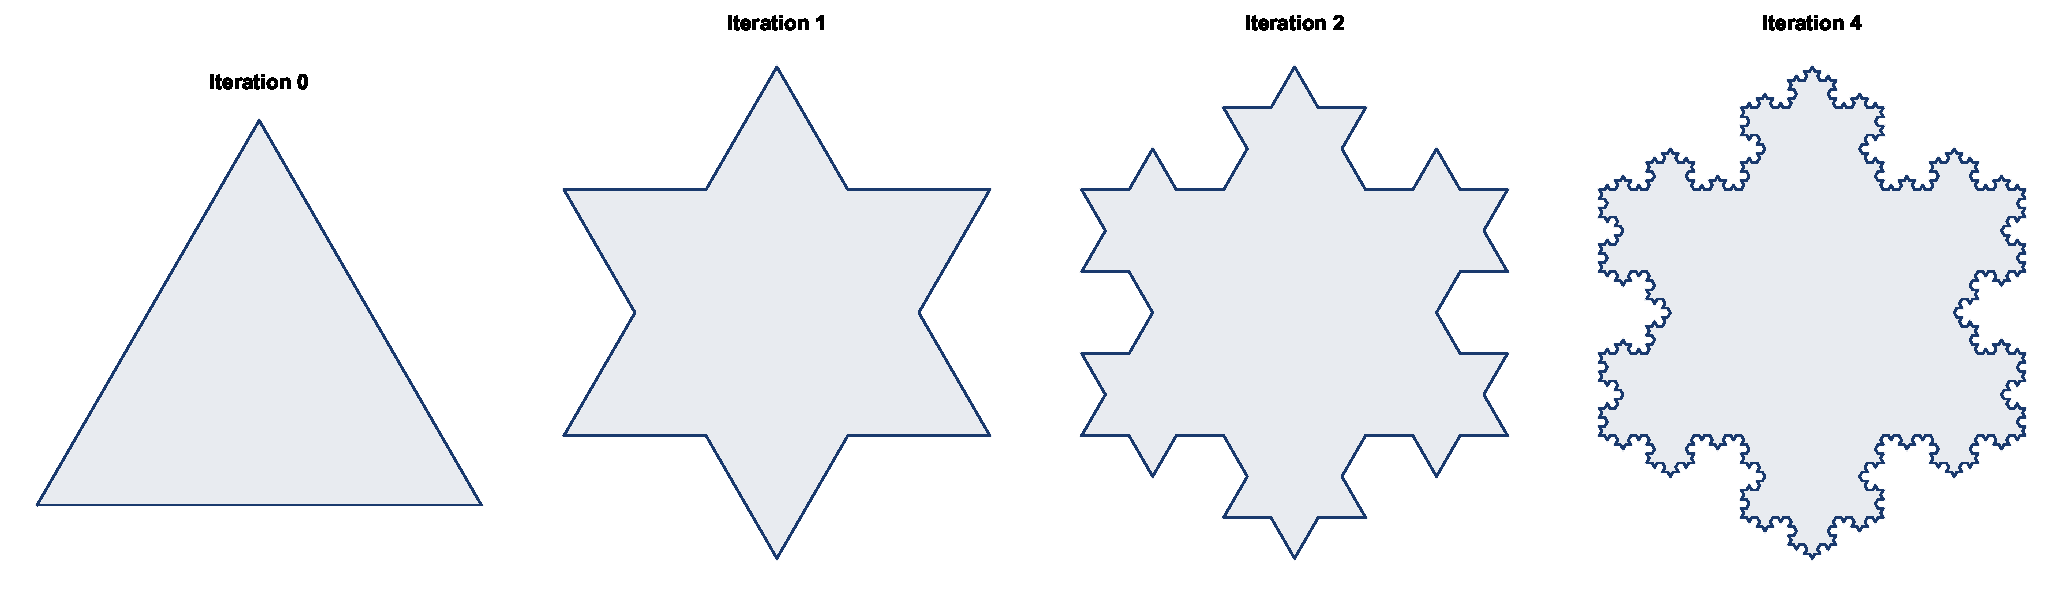
\includegraphics[width=\linewidth]{ch_fmh_koch_snowflake.pdf}\\[2pt]
{\scriptsize\textcolor{MediumGray}{\textbf{Fulgul Koch} (1904) --- la fiecare iterație fiecare segment este înlocuit cu 4 segmente de lungime $1/3$. Lungime infinită, arie finită.}}\\[3pt]
\begin{itemize}\setlength{\itemsep}{0pt}
    \item \scriptsize Dimensiune fractală: $D = \log 4 / \log 3 \approx 1{,}262$
\end{itemize}
\figql{SFM\_ch\_fmh\_fractals: koch\_snowflake}{https://github.com/QuantLet/Stat_fin_markets/tree/master/Quantlets/SFM_ch_fmh}
\end{column}
\end{columns}
\end{cminipage}
\end{frame}

\slidelevel{Y3}
\begin{frame}[shrink=20]{Triunghiul Sierpinski și curba dragonului}
\begin{cminipage}{0.96\textwidth}
\begin{columns}[T]
\begin{column}{0.48\textwidth}
\centering
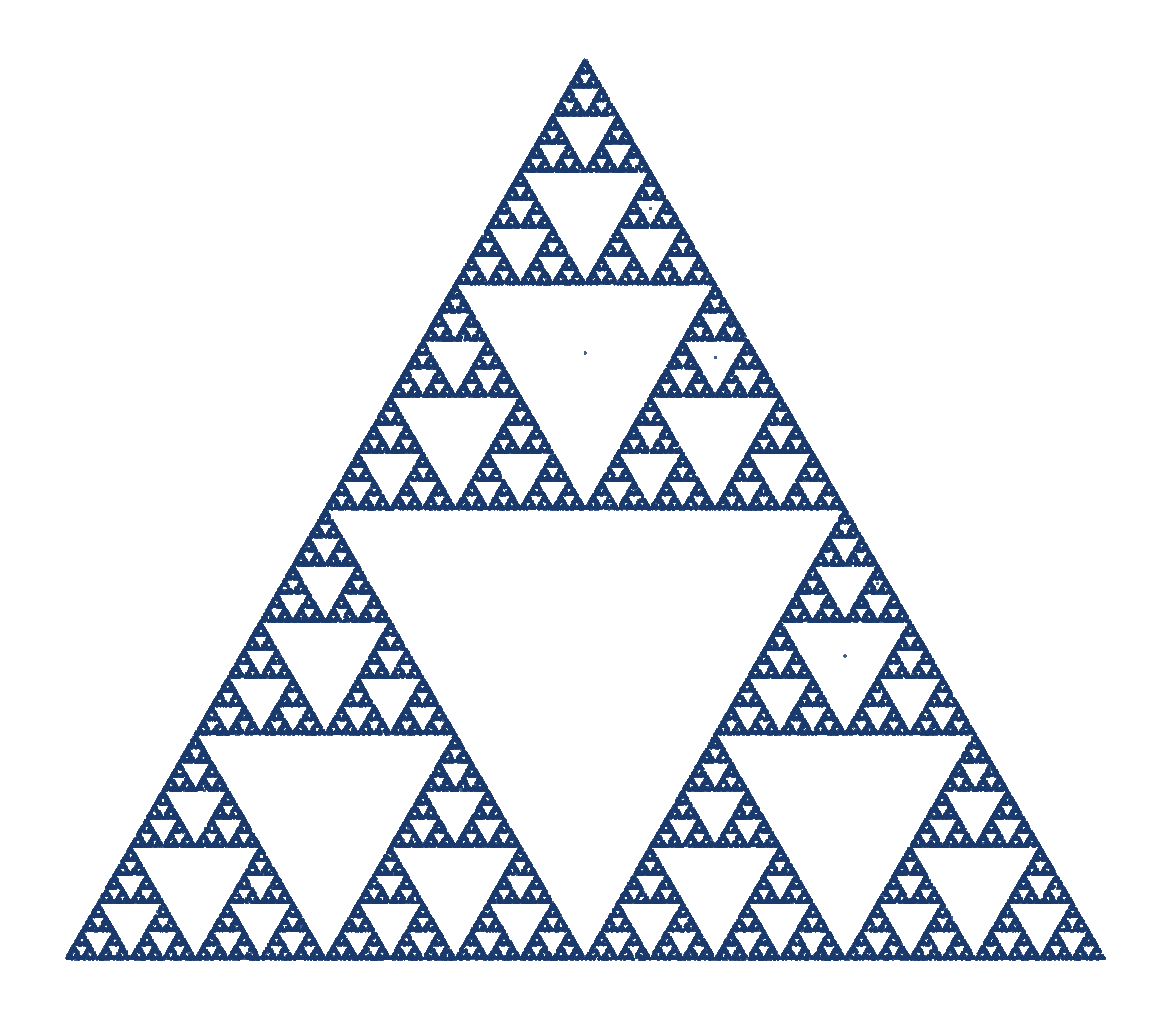
\includegraphics[height=4.6cm,keepaspectratio]{ch_fmh_sierpinski.pdf}\\[1pt]
{\tiny\textcolor{MediumGray}{\textbf{Sierpinski} --- chaos game; $D = \log 3/\log 2 \approx 1{,}585$.}}\\[1pt]
\figql{SFM\_ch\_fmh\_fractals: sierpinski}{https://github.com/QuantLet/Stat_fin_markets/tree/master/Quantlets/SFM_ch_fmh}
\end{column}
\begin{column}{0.50\textwidth}
\centering
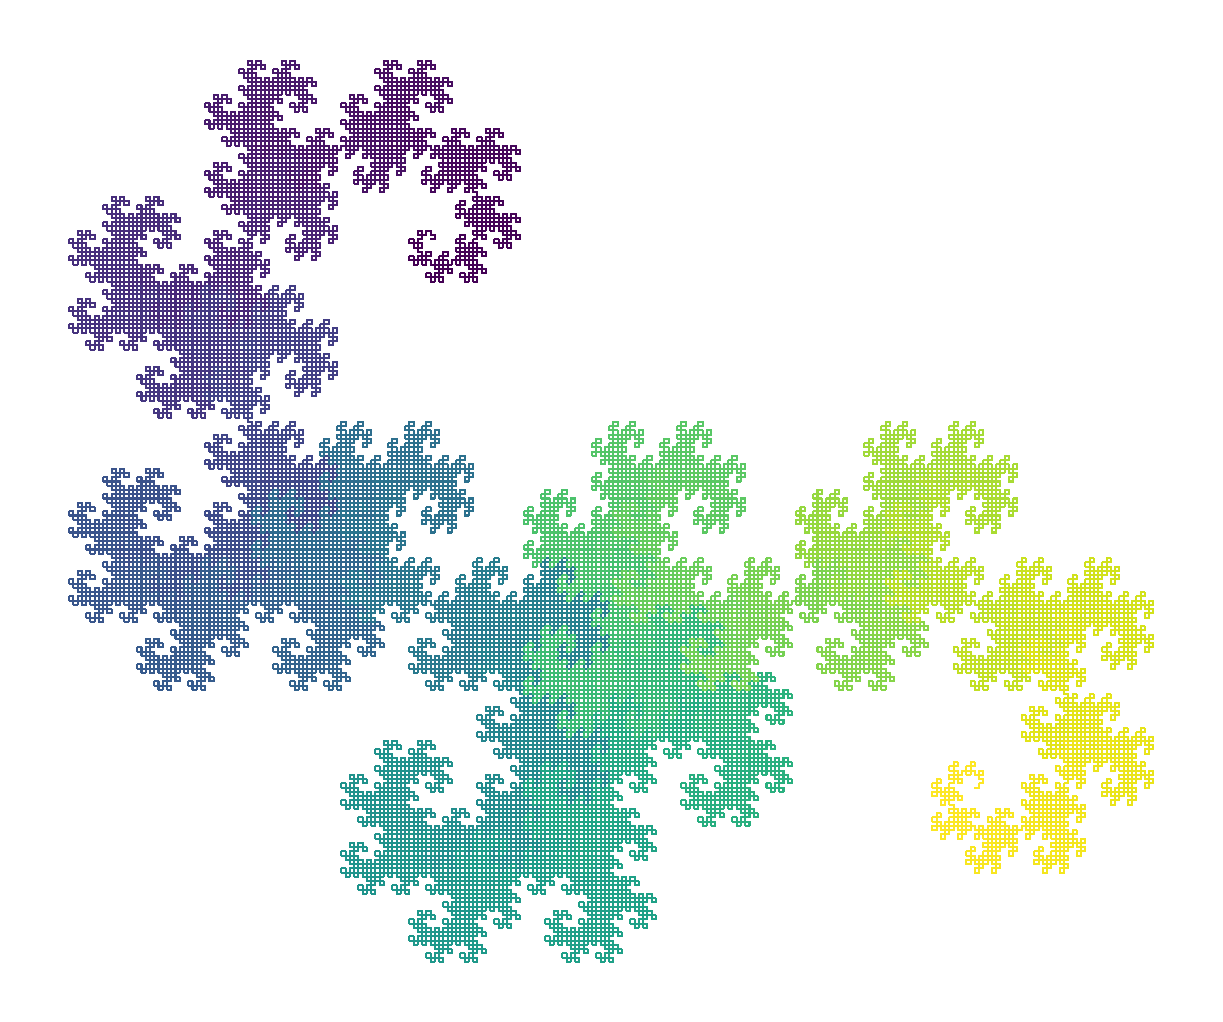
\includegraphics[height=4.6cm,keepaspectratio]{ch_fmh_dragon_curve.pdf}\\[1pt]
{\tiny\textcolor{MediumGray}{\textbf{Curba dragonului} (Heighway) --- pliere succesivă; $D \approx 2$.}}\\[1pt]
\figql{SFM\_ch\_fmh\_fractals: dragon\_curve}{https://github.com/QuantLet/Stat_fin_markets/tree/master/Quantlets/SFM_ch_fmh}
\end{column}
\end{columns}
\end{cminipage}
\end{frame}

\slidelevel{Y3}
\begin{frame}[shrink=10]{Țărmurile fractale: ,,Cât de lungă este coasta Britaniei?''}
\begin{cminipage}{0.96\textwidth}
\begin{columns}[T]
\begin{column}{0.40\textwidth}
\begin{itemize}\setlength{\itemsep}{1pt}
    \item Mandelbrot (1967, \textit{Science}): lungimea măsurată depinde de \textbf{rigla} folosită
    \item Cu o riglă de $\varepsilon$ km, lungimea este:
    \[
        L(\varepsilon) \propto \varepsilon^{1 - D}
    \]
    \item $D > 1$ $\Rightarrow$ $L \to \infty$ când $\varepsilon \to 0$
    \item Coasta Britaniei: $D \approx 1{,}25$
    \item Coasta Norvegiei: $D \approx 1{,}52$ (mai zimțată!)
    \item \textbf{Analogia financiară:} graficul prețului $P(t)$ are dimensiune fractală $D = 2 - H$
    \begin{itemize}\setlength{\itemsep}{0pt}
        \item $H = 0{,}5 \Rightarrow D = 1{,}5$ (mers aleator standard)
        \item $H > 0{,}5 \Rightarrow D < 1{,}5$ (traiectorie mai netedă)
        \item $H < 0{,}5 \Rightarrow D > 1{,}5$ (traiectorie mai zimțată)
    \end{itemize}
\end{itemize}
\end{column}
\begin{column}{0.58\textwidth}
\centering
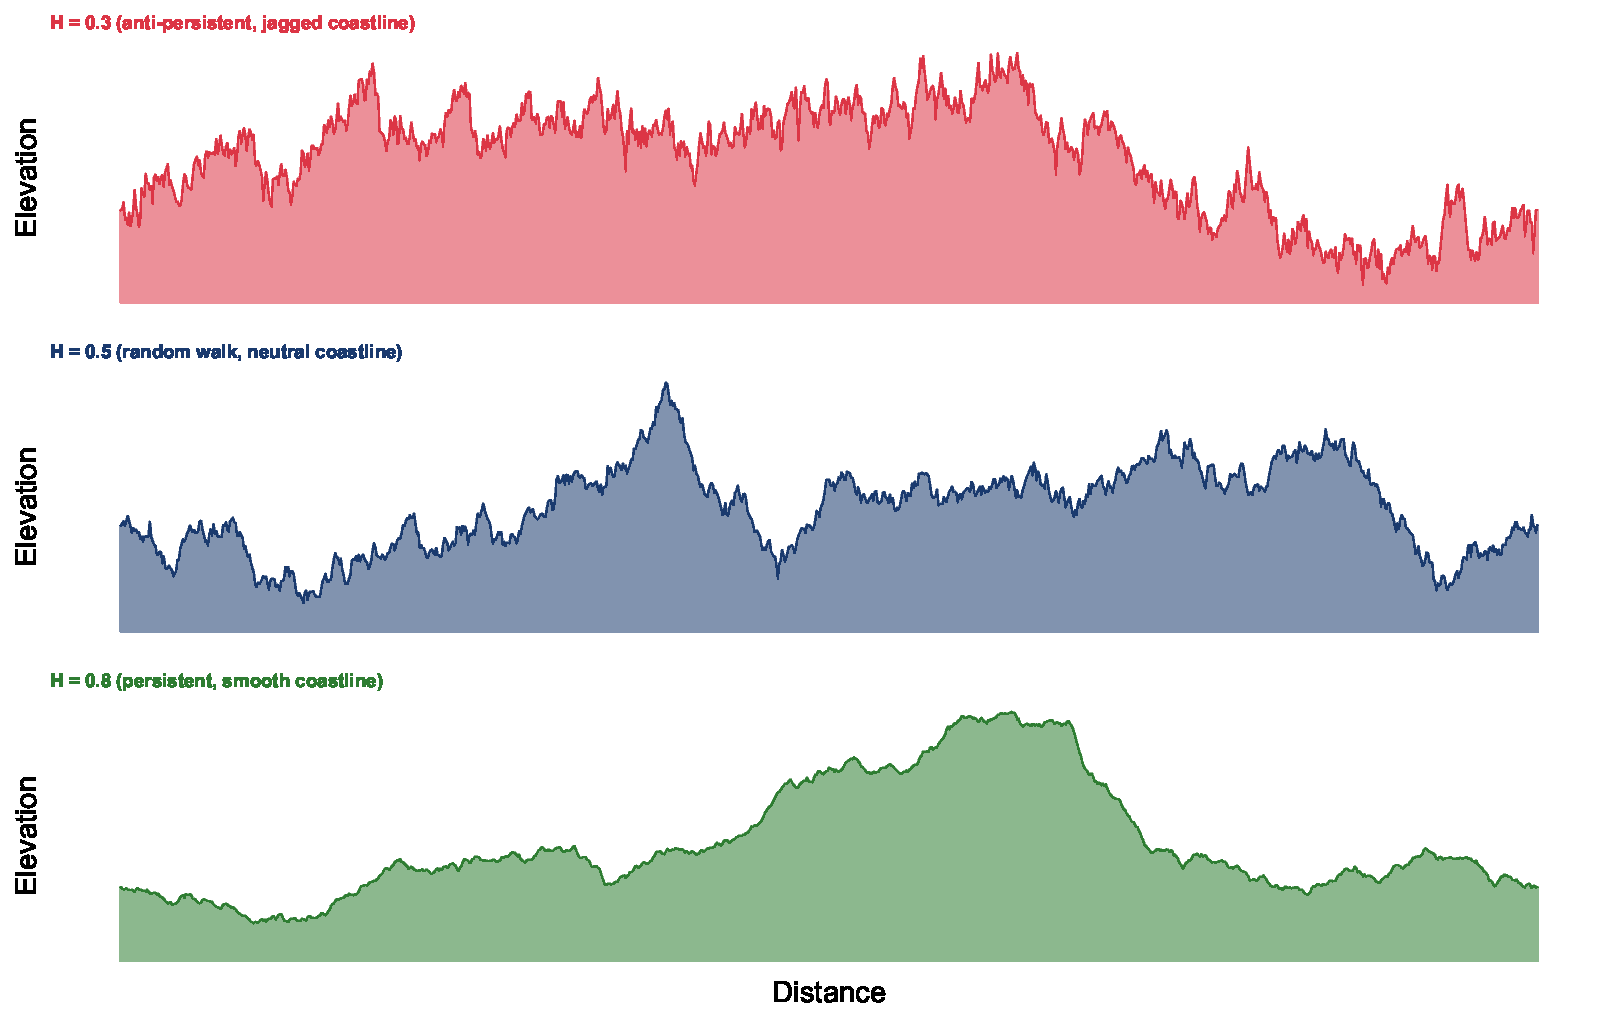
\includegraphics[width=\linewidth]{ch_fmh_coastline.pdf}\\[2pt]
{\scriptsize\textcolor{MediumGray}{\textit{Țărmuri sintetice generate cu deplasare aleatoare la mijloc, pentru trei valori ale exponentului Hurst.}}}
\figql{SFM\_ch\_fmh\_fractals: coastline}{https://github.com/QuantLet/Stat_fin_markets/tree/master/Quantlets/SFM_ch_fmh}
\end{column}
\end{columns}
\end{cminipage}
\end{frame}

\slidelevel{Y3}
\begin{frame}[shrink=10]{Fulger, descărcare electrică (Lightning, electric discharge)}
\begin{cminipage}{0.95\textwidth}
\begin{columns}[T]
\begin{column}{0.42\textwidth}
\begin{itemize}\setlength{\itemsep}{1pt}
    \item Descărcările electrice (fulger, scântei, figuri Lichtenberg) sunt \textbf{ramificații fractale}
    \item Modelate prin \textbf{Diffusion-Limited Aggregation (DLA)}, Witten \& Sander (1981)
    \item Algoritm: particule fac mers aleator (random walk) și se ,,lipesc'' la primul contact cu cluster-ul
    \item Dimensiune fractală: $D \approx 1{,}71$ în 2D, $D \approx 2{,}5$ în 3D
    \item \textbf{Principii similare} apar în:
    \begin{itemize}\setlength{\itemsep}{0pt}
        \item Creșterea cristalelor de gheață (snowflakes)
        \item Electrodepunere
        \item Bacterii (\textit{Bacillus subtilis})
        \item Răspândirea avalanșelor pe piețe (cascading liquidations)
    \end{itemize}
    \item \textbf{Conexiune financiară}: răspândirea panicii într-o rețea de traderi e analogă DLA
\end{itemize}
\end{column}
\begin{column}{0.55\textwidth}
\centering
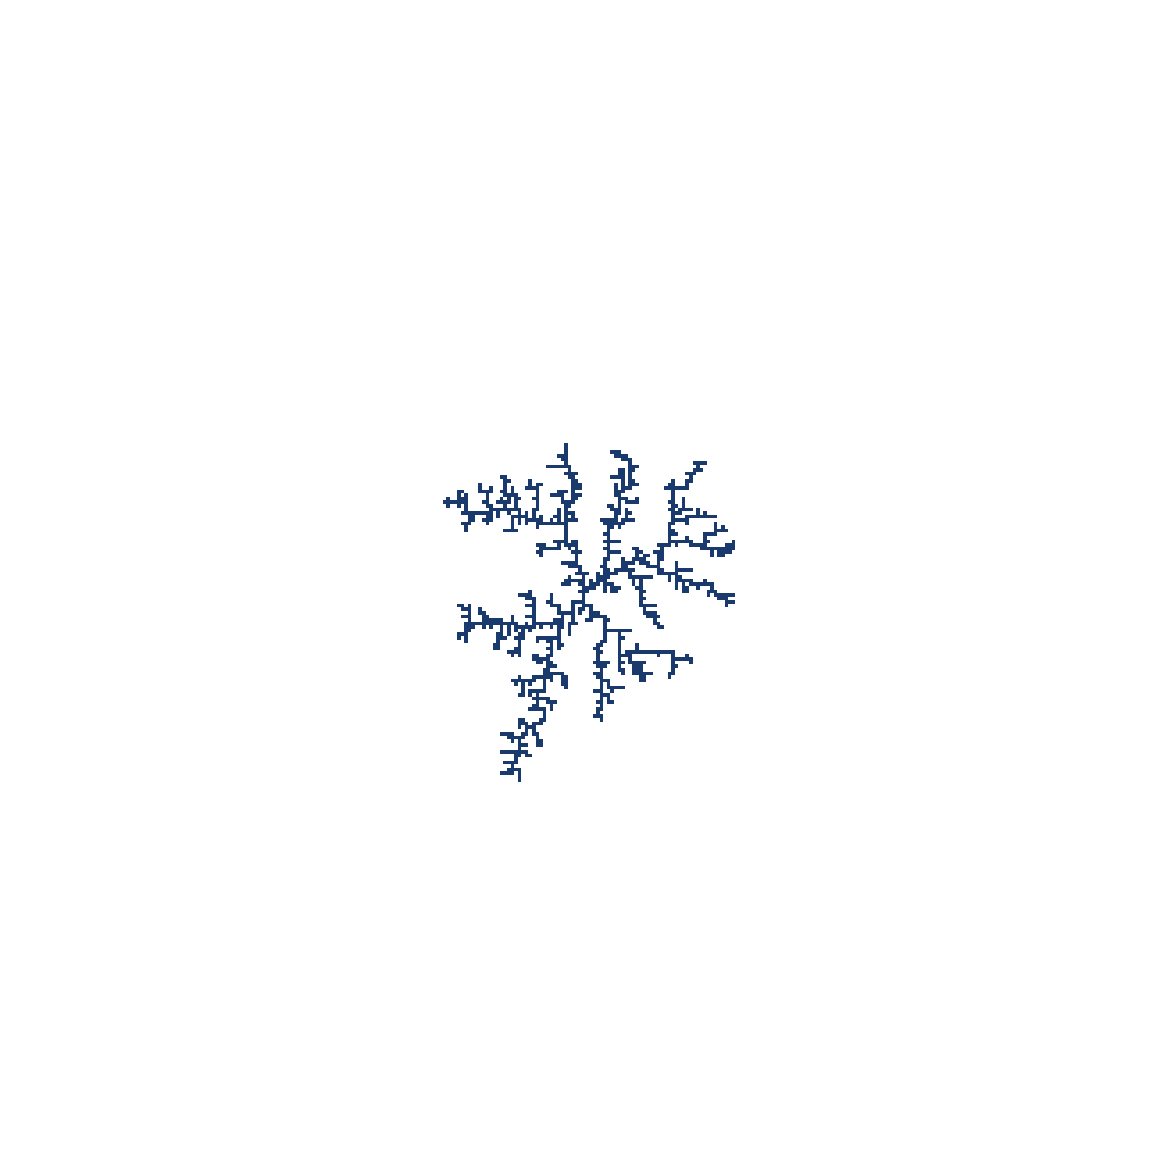
\includegraphics[width=0.95\linewidth]{ch_fmh_dla.pdf}\\[2pt]
{\scriptsize\textcolor{MediumGray}{\textit{Cluster DLA generat prin agregare a $\sim$1700 particule. Structura ramificată reproduce fenomene din natură.}}}
\figql{SFM\_ch\_fmh\_extra: dla}{https://github.com/QuantLet/Stat_fin_markets/tree/master/Quantlets/SFM_ch_fmh}
\end{column}
\end{columns}
\end{cminipage}
\end{frame}

\slidelevel{Y3}
\begin{frame}[shrink=10]{Rețele de râuri și sisteme circulatorii (River networks \& vascular systems)}
\begin{cminipage}{0.95\textwidth}
\begin{columns}[T]
\begin{column}{0.42\textwidth}
\begin{itemize}\setlength{\itemsep}{1pt}
    \item \textbf{Rețele de râuri (river networks)}: la fiecare confluență, un râu mare = două sau mai multe râuri mai mici
    \item \textbf{Legile Horton (Horton's laws, 1945)}: relații de scalare între ordine de râuri
    \item \textbf{Sisteme vasculare} (\textit{circulatory systems}): bronhii pulmonare ($\sim$23 nivele), capilare, neuroni
    \item \textbf{Eficiență energetică}: ramificarea fractală \textbf{minimizează} energia de transport pe unitatea de masă
    \item \textbf{Legea West-Brown-Enquist}: rata metabolică $\propto M^{3/4}$ (West, Brown \& Enquist, 1997) — \textbf{dimensiune fractală a rețelei vasculare}
    \item \textbf{Conexiune financiară}: rețele de plăți, lanțuri de creditori, propagarea șocurilor în sistemul financiar
\end{itemize}
\end{column}
\begin{column}{0.55\textwidth}
\centering

\includegraphics[width=0.85\linewidth]{ch_fmh_river_network.pdf}\\[2pt]
{\scriptsize\textcolor{MediumGray}{\textit{Rețea fractală generată prin ramificare aleatoare; structuri similare apar în delte de râuri și plămâni.}}}
\figql{SFM\_ch\_fmh\_extra: river\_network}{https://github.com/QuantLet/Stat_fin_markets/tree/master/Quantlets/SFM_ch_fmh}
\end{column}
\end{columns}
\end{cminipage}
\end{frame}

\slidelevel{Y3}
\begin{frame}[shrink=15]{Alți fractali din natură (Other natural fractals)}
\begin{cminipage}{0.95\textwidth}
\renewcommand{\arraystretch}{1.25}
\begin{center}
\small
\begin{tabular}{lll}
\toprule
\textbf{Obiect natural} & \textbf{Dimensiune fractală $D$} & \textbf{Mecanism} \\
\midrule
Coasta Britaniei & $\approx 1{,}25$ & Eroziune diferențială \\
Coasta Norvegiei & $\approx 1{,}52$ & Glaciație, fiorduri \\
Munții Alpine (skyline) & $\approx 1{,}40$ & Eroziune și ridicare tectonică \\
Norii (cumulus) & $\approx 1{,}35$--$1{,}40$ & Convecție, turbulență \\
Suprafața creierului uman & $\approx 2{,}79$ & Maximizare suprafață în volum mic \\
Bronhii pulmonare & $\approx 2{,}97$ & Ramificare fractală pentru schimb O$_2$ \\
Vase de sânge & $\approx 2{,}7$ & Optimizare West-Brown-Enquist \\
Romanesco (varză broccoli) & $\approx 2{,}66$ & Spirala Fibonacci, auto-similaritate \\
Galaxii (distribuția spațială) & $\approx 1{,}2$--$2{,}0$ & Gravitație + expansiune \\
Lemnul (anular structure) & $\approx 1{,}28$ & Creștere stratificată \\
Plămânii (volum total) & $\approx 2{,}97$ & Maximizare suprafață \\
Rețele neuronale & $\approx 1{,}68$ & Branching axonal \\
\bottomrule
\end{tabular}
\end{center}
\vspace{0.1cm}
\begin{itemize}\setlength{\itemsep}{0pt}
    \item Patternuri \textbf{universale} cu dimensiuni fractale tipice $D \in [1{,}2;\, 3{,}0]$
    \item Mecanism comun: \textbf{procese stocastice cu memorie} (Markov, fBm, multiplicative cascades)
\end{itemize}
\end{cminipage}
\end{frame}

\slidelevel{MSc}
\begin{frame}[shrink=15]{Muzica și limbajul ca fractali (Music and language as fractals)}
\begin{cminipage}{0.95\textwidth}
\begin{columns}[T]
\begin{column}{0.50\textwidth}
\begin{block}{Muzică (Voss \& Clarke, 1975)}
\begin{itemize}\setlength{\itemsep}{0pt}
    \item Densitatea spectrală a fluctuațiilor în pitch și loudness $f(\omega) \sim 1/\omega$
    \item Numit \textbf{$1/f$ noise} (zgomot pink)
    \item Bach, Mozart, Beatles, Beethoven: cu toții în regim ,,$1/f$''
    \item Muzica complet aleatoare ($1/f^0$, white noise) sună neplăcut
    \item Muzica complet predictibilă ($1/f^2$, brown noise) sună plictisitor
    \item ,,$1/f$'' = balanța estetică optimă!
\end{itemize}
\end{block}
\end{column}
\begin{column}{0.46\textwidth}
\begin{block}{Limbaj (Mandelbrot, 1953)}
\begin{itemize}\setlength{\itemsep}{0pt}
    \item Frecvența cuvintelor: \textbf{Legea Zipf}
    \[
        \text{frecvență} \propto \frac{1}{\text{rang}^\alpha}
    \]
    cu $\alpha \approx 1$ pentru limbi naturale
    \item Distribuție \textbf{cu coadă grea} (heavy-tailed)
    \item \textbf{Mandelbrot 1953}: a propus prima generalizare:
    \[
        f_n = \frac{C}{(n + \beta)^\alpha}
    \]
    \item Aplicare modernă: distribuții site web, retweet, citații științifice
\end{itemize}
\end{block}
\end{column}
\end{columns}

\vspace{0.2cm}

\begin{alertblock}{Conexiunea cu finanțele}
\begin{itemize}\setlength{\itemsep}{0pt}
    \item Randamentele bursiere urmează \textbf{aceleași legi de scalare}
    \item \textbf{Cozi grele Pareto}: distribuții cu power-law tails
\end{itemize}
\end{alertblock}
\end{cminipage}
\end{frame}

\slidelevel{Y3}
\begin{frame}[shrink=10]{Prețul ca fractal (Price as a fractal)}
\begin{cminipage}{0.95\textwidth}
\begin{itemize}\setlength{\itemsep}{0pt}
    \item Mandelbrot (1963, 2004): \textbf{,,Markets are turbulent like fluids and fractal like coastlines.''}
    \item Privind un grafic intraday vs daily vs weekly $\Rightarrow$ același tip de variabilitate
    \item Fără bare temporale (tick-removed), nu poți spune \textbf{ce frecvență} privești
\end{itemize}

\vspace{0.1cm}
\centering
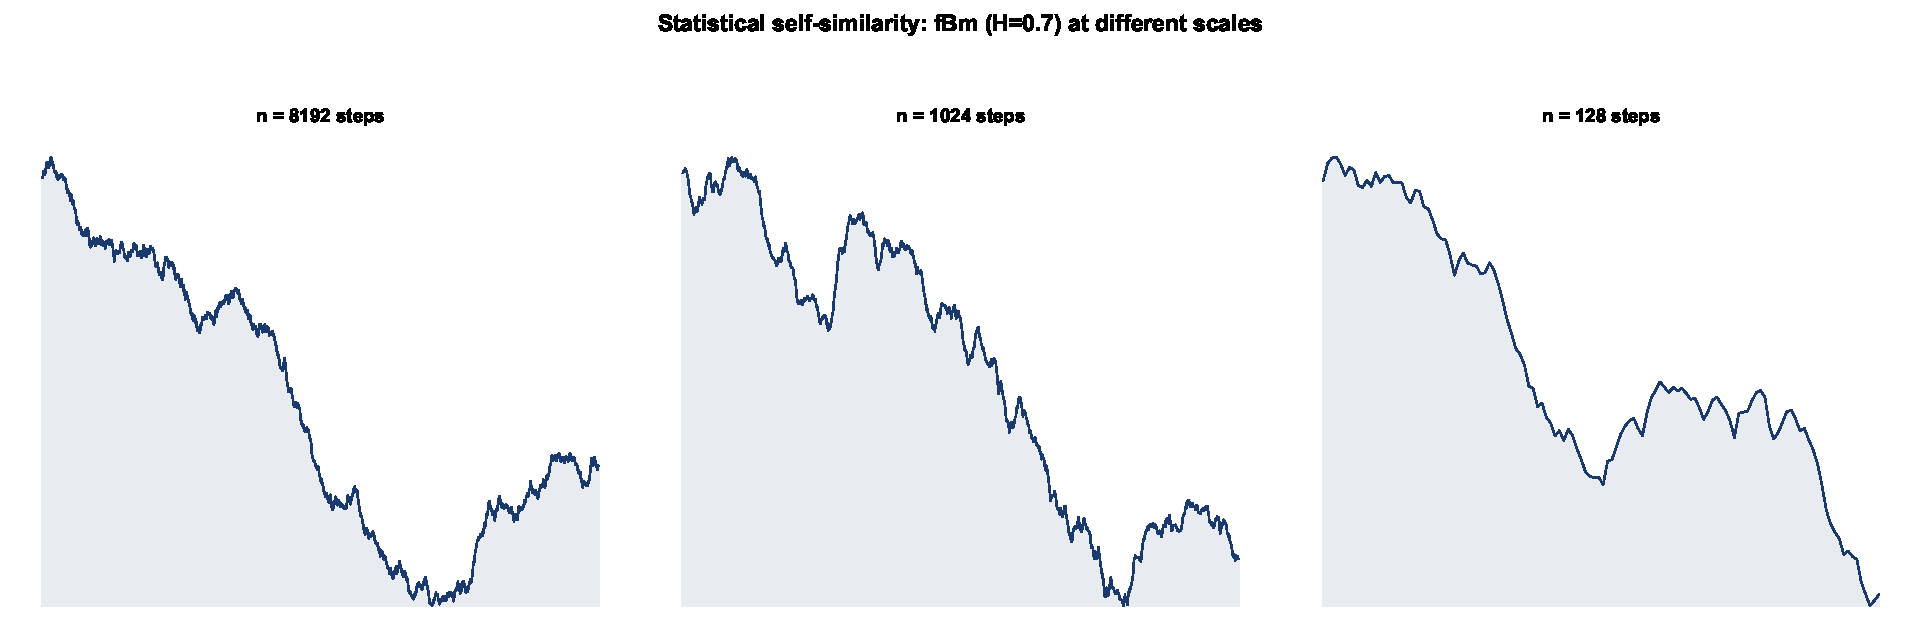
\includegraphics[height=4.8cm,keepaspectratio]{ch_fmh_selfsimilarity.pdf}\\[2pt]
{\scriptsize\textcolor{MediumGray}{\textit{Aceeași traiectorie fBm la trei nivele de zoom — structura statistică se conservă. Aceasta este }auto-similaritatea statistică\textit{ care caracterizează randamentele bursiere reale.}}}
\figql{SFM\_ch\_fmh\_fractals: selfsimilarity}{https://github.com/QuantLet/Stat_fin_markets/tree/master/Quantlets/SFM_ch_fmh}
\end{cminipage}
\end{frame}

%#############################################################################
% RESTRUCTURARE TASK 1: secțiunea-orfan "Ce este dimensiunea fractală?" (1 slide)
% a fost absorbită aici ca prim frame, pentru a stabili definiția simplă
% înainte de derivările formale (Cantor, box-counting, Hausdorff).
\section{Autosimilaritate și dimensiune fractală}
%#############################################################################

% PRIMER mutat la începutul §2 Fractali în natură.
\slidelevel{Y3}
\begin{frame}[shrink=15]{Mulțimea Cantor: primul fractal}
\begin{cminipage}{0.96\textwidth}
\begin{columns}[T]
\begin{column}{0.45\textwidth}
\begin{defn}[Mulțimea Cantor]
Se pornește cu $C_0 = [0, 1]$. La fiecare pas, fiecare interval își scoate \textbf{treimea de mijloc}:
\[
    C_{k+1} = \bigcup_{[a,b] \in C_k} \left( \left[a, a + \tfrac{b-a}{3}\right] \cup \left[b - \tfrac{b-a}{3}, b\right] \right)
\]
Mulțimea Cantor: $C = \bigcap_{k=0}^{\infty} C_k$.
\end{defn}

\begin{itemize}\setlength{\itemsep}{1pt}
    \item Conține o \textbf{infinitate} nenumărabilă de puncte
    \item \textbf{Lungime totală} $= 0$
    \item \textbf{Dimensiune fractală}:
    \[
        D = \frac{\log 2}{\log 3} \approx 0{,}631
    \]
    \item \textbf{Autosimilară exact}: fiecare jumătate $C \cap [0, 1/3]$ este o copie scalată $\times 1/3$ a întregului $C$
\end{itemize}
\end{column}
\begin{column}{0.52\textwidth}
\centering
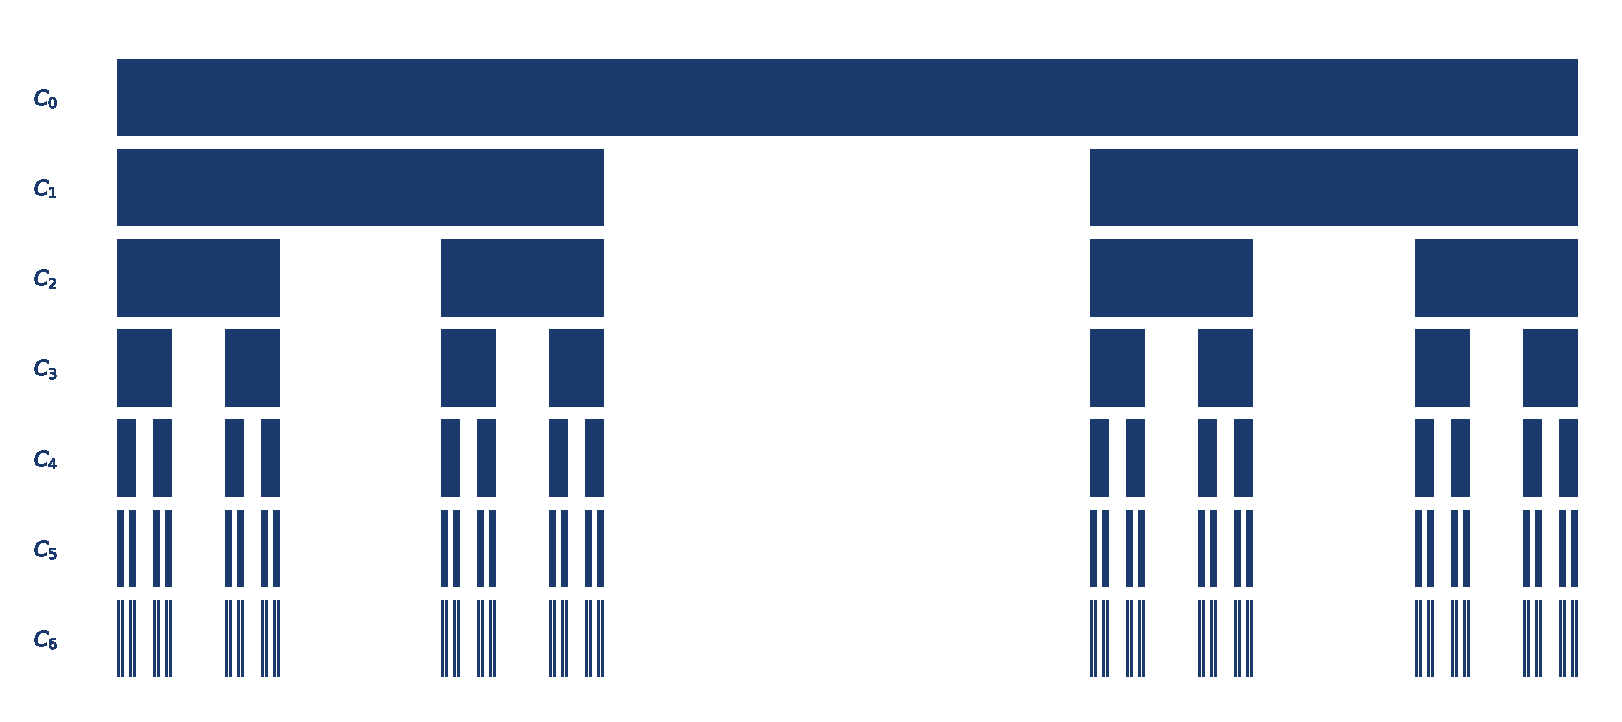
\includegraphics[width=\linewidth]{ch_fmh_cantor.pdf}\\[3pt]
{\scriptsize\textcolor{MediumGray}{\textit{Primele 7 iterații în construcția mulțimii Cantor.}}}
\figql{SFM\_ch\_fmh\_fractals: cantor}{https://github.com/QuantLet/Stat_fin_markets/tree/master/Quantlets/SFM_ch_fmh}
\end{column}
\end{columns}
\end{cminipage}
\end{frame}

\slidelevel{MSc}
\begin{frame}[shrink=20]{Autosimilaritate statistică}
\begin{cminipage}{0.95\textwidth}
\begin{defn}[Proces autosimilar]
Un proces stocastic $\{X(t)\}_{t \geq 0}$ este \textbf{autosimilar} cu indicele $H > 0$ dacă pentru orice $c > 0$:
\[
    \{X(ct)\}_{t \geq 0} \stackrel{d}{=} \{c^H X(t)\}_{t \geq 0}
\]
unde $\stackrel{d}{=}$ înseamnă egalitatea \textit{tuturor} distribuțiilor finit-dimensionale.
\end{defn}

\begin{columns}[T]
\begin{column}{0.50\textwidth}
\begin{itemize}\setlength{\itemsep}{0pt}
    \item Parametrul $H$ se numește \textbf{exponent Hurst} sau \textbf{exponent de autosimilaritate}
    \item \textbf{Implicații pentru randamente}: dacă $\ln P(t)$ este $H$-autosimilar, scalarea timpului cu $c$ $\Leftrightarrow$ scalarea randamentelor cu $c^H$
    \item \textbf{Legea de scalare a volatilității}:
    \[
        \sigma(\Delta) = \sigma(1) \cdot \Delta^{H}
    \]
    \item Sub EMH ($H = 0{,}5$): regula clasică a rădăcinii pătrate $\sigma(\Delta) = \sigma(1) \sqrt{\Delta}$
    \item $H \neq 0{,}5$ $\Rightarrow$ \textbf{evidență contra EMH}
\end{itemize}
\end{column}
\begin{column}{0.48\textwidth}
\centering
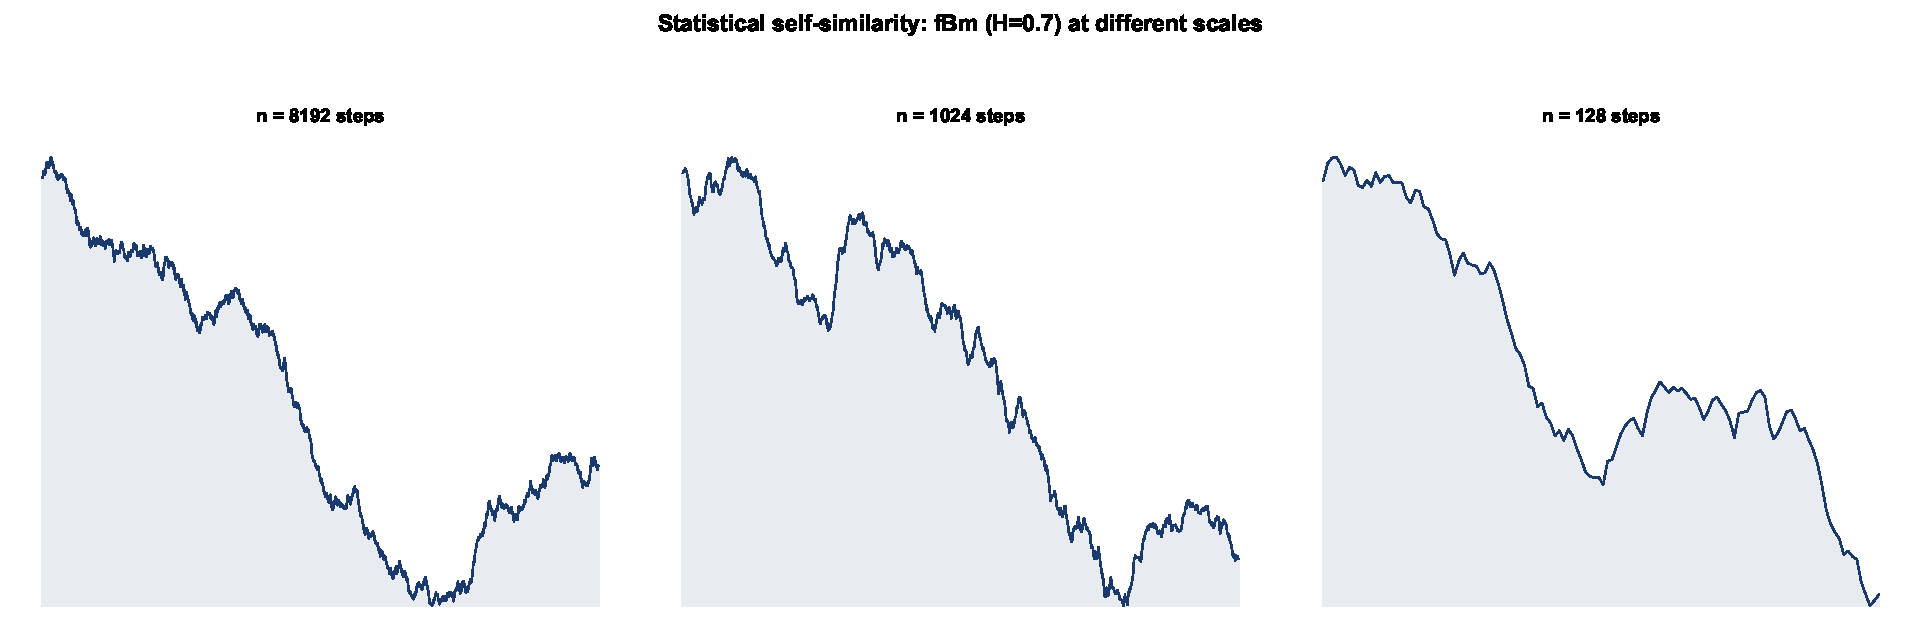
\includegraphics[width=\linewidth]{ch_fmh_selfsimilarity.pdf}\\[3pt]
{\scriptsize\textcolor{MediumGray}{\textit{Aceeași traiectorie fBm la trei nivele de zoom — structura statistică se conservă.}}}
\figql{SFM\_ch\_fmh\_fractals: selfsimilarity}{https://github.com/QuantLet/Stat_fin_markets/tree/master/Quantlets/SFM_ch_fmh}
\end{column}
\end{columns}
\end{cminipage}
\end{frame}

\slidelevel{MSc}
\begin{frame}[shrink=15]{Dimensiunea fractală box-counting}
\begin{cminipage}{0.95\textwidth}
\begin{defn}[Dimensiune box-counting]
Fie $S \subset \R^d$ o mulțime mărginită și $N(\varepsilon)$ numărul minim de cuburi de latură $\varepsilon$ necesare pentru a acoperi $S$. Dimensiunea \textbf{box-counting} (Minkowski-Bouligand):
\[
    D_{\text{box}} = \lim_{\varepsilon \to 0^+} \frac{\log N(\varepsilon)}{\log(1/\varepsilon)}
\]
\end{defn}

\begin{itemize}\setlength{\itemsep}{1pt}
    \item Estimată empiric prin \textbf{regresie liniară} a $\log N(\varepsilon)$ pe $\log(1/\varepsilon)$
    \item Pentru obiecte clasice: punct $D=0$, segment $D=1$, pătrat $D=2$
    \item Pentru fractali: $D$ \textbf{neîntreg}; cuantifică ,,neregularitatea''
\end{itemize}

\vspace{0.1cm}
\centering
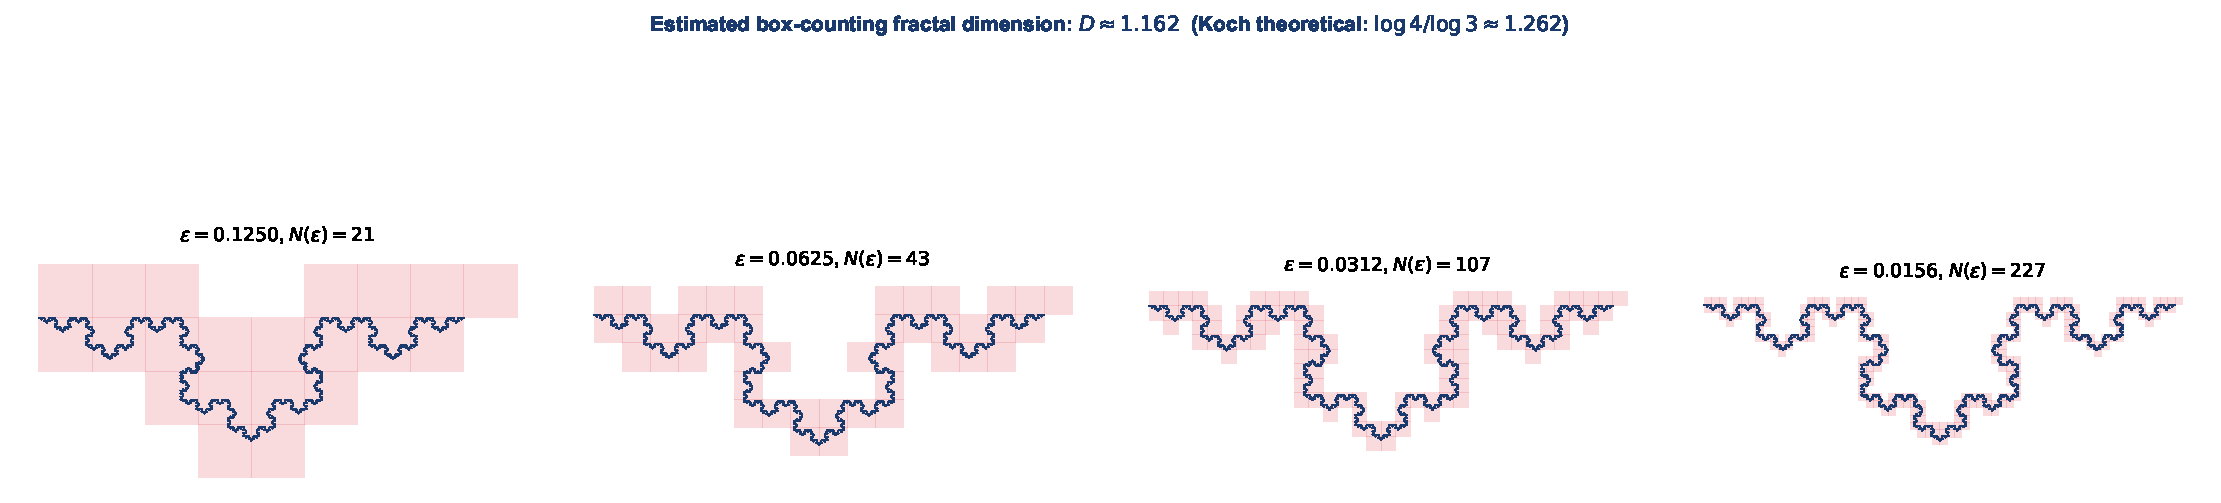
\includegraphics[width=0.95\linewidth]{ch_fmh_boxcount.pdf}
\figql{SFM\_ch\_fmh\_fractals: boxcount}{https://github.com/QuantLet/Stat_fin_markets/tree/master/Quantlets/SFM_ch_fmh}
\end{cminipage}
\end{frame}

\slidelevel{MSc}
\begin{frame}[shrink=20]{Dimensiunea Hausdorff (Hausdorff dimension)}
\begin{cminipage}{0.95\textwidth}
\begin{defn}[Măsura și dimensiunea Hausdorff]
Pentru $S \subset \R^n$ și $d \geq 0$, măsura Hausdorff:
\[
    \mathcal{H}^d(S) = \lim_{\delta \to 0^+} \inf \Bigl\{ \sum_{i} (\text{diam } U_i)^d : \text{diam } U_i < \delta \Bigr\}
\]
\textbf{Dimensiunea Hausdorff}: $\dim_H(S) = \inf \{d : \mathcal{H}^d(S) = 0\}$.
\end{defn}

\begin{itemize}\setlength{\itemsep}{0pt}
    \item \textbf{Riguroasă} matematic, greu de calculat empiric
    \item Pentru fractali ,,bine-comportați'': $\dim_H = D_{\text{box}}$
    \item \textbf{Exemple cheie}: Cantor $\approx 0{,}631$ \quad Koch $\approx 1{,}262$ \quad Sierpinski $\approx 1{,}585$ \quad Frontiera Mandelbrot $= 2$ (Shishikura, 1998)
    \item În finanțe: $\dim_H$ a graficului prețului $= 2 - H$ (Mandelbrot 1968)
\end{itemize}
\end{cminipage}
\end{frame}

\slidelevel{MSc}
\begin{frame}[shrink=15]{Dimensiuni alternative (Alternative dimensions)}
\begin{cminipage}{0.95\textwidth}
\renewcommand{\arraystretch}{1.3}
\begin{center}
\small
\begin{tabular}{lll}
\toprule
\textbf{Tip de dimensiune} & \textbf{Definiție} & \textbf{Aplicație} \\
\midrule
Hausdorff $D_H$ & Vezi slide anterior & Standard matematic, dificilă numeric \\
Box-counting $D_{\text{box}}$ & $\lim \frac{\log N(\varepsilon)}{\log(1/\varepsilon)}$ & Cea mai folosită empiric \\
Similaritate $D_S$ & $\sum_{i=1}^N r_i^{D_S} = 1$ & Pentru IFS auto-similare \\
Informație $D_I$ & $-\lim \frac{\sum p_i \log p_i}{\log \varepsilon}$ & Distribuție de masă pe fractal \\
Corelație $D_C$ & $\lim \frac{\log C(\varepsilon)}{\log \varepsilon}$ & Time-series chaos (Grassberger 1983) \\
$q$-dimensiune $D_q$ & $\lim \frac{\log \sum p_i^q}{(q-1) \log \varepsilon}$ & Generalizează multifractal \\
Spectru $f(\alpha)$ & Legendre$(\tau(q))$ & Multifractalitate completă \\
\bottomrule
\end{tabular}
\end{center}
\vspace{0.2cm}
\begin{itemize}\setlength{\itemsep}{0pt}
    \item Pentru \textbf{monofractali}: toate dimensiunile coincid: $D_H = D_{\text{box}} = D_q$ pentru orice $q$
    \item Pentru \textbf{multifractali}: $D_q$ depinde de $q$ $\Rightarrow$ \textbf{spectru de dimensiuni}
    \item \textbf{Identitate fundamentală}: $D_q$ este \textbf{ne-crescătoare} în $q$
\end{itemize}
\end{cminipage}
\end{frame}

\slidelevel{MSc}
\begin{frame}{Estimarea empirică a dimensiunii box-counting}
\begin{cminipage}{0.95\textwidth}
\centering
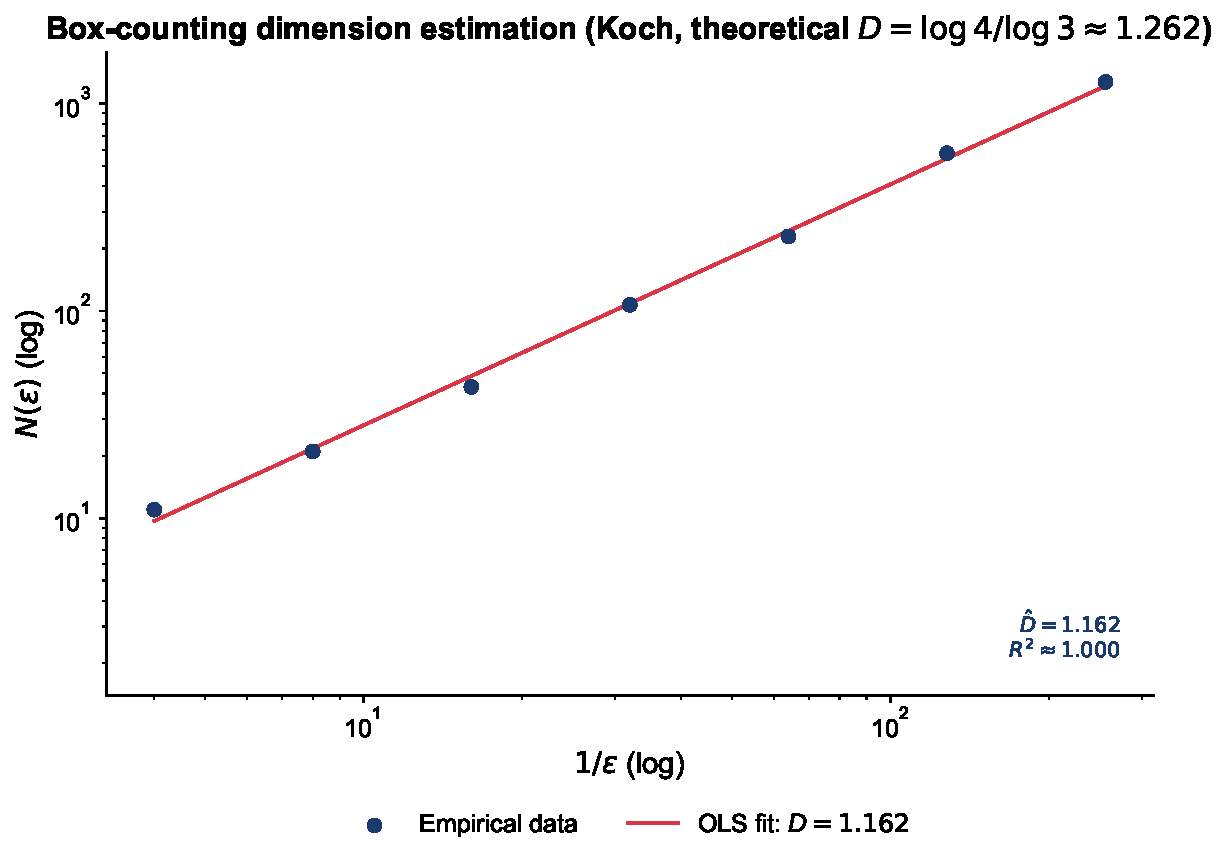
\includegraphics[height=5.2cm,keepaspectratio]{ch_fmh_boxcount_reg.pdf}\\[3pt]
{\scriptsize\textcolor{MediumGray}{\textit{Regresia log-log $\log N(\varepsilon) = D \log(1/\varepsilon) + c$ pentru curba Koch. Estimarea $\hat{D}$ corespunde valorii teoretice $\log 4/\log 3 \approx 1.262$.}}}
\figql{SFM\_ch\_fmh\_extra: boxcount\_reg}{https://github.com/QuantLet/Stat_fin_markets/tree/master/Quantlets/SFM_ch_fmh}
\end{cminipage}
\end{frame}

\slidelevel{PhD}
\begin{frame}[shrink=15]{Auto-similaritate exactă vs statistică (Exact vs statistical self-similarity)}
\begin{cminipage}{0.95\textwidth}
\begin{columns}[T]
\begin{column}{0.50\textwidth}
\begin{block}{Auto-similaritate exactă (deterministă)}
\begin{itemize}\setlength{\itemsep}{0pt}
    \item Mulțimea este unirea finită de copii la scară redusă a sieși
    \[
        S = \bigcup_{i=1}^{N} f_i(S), \quad f_i \text{ contracții}
    \]
    \item Exemple: Cantor, Koch, Sierpinski, Mandelbrot
    \item Dimensiunea de similaritate $D_S$ via ec. Moran:
    \[
        \sum_{i=1}^N r_i^{D_S} = 1
    \]
\end{itemize}
\end{block}
\end{column}
\begin{column}{0.48\textwidth}
\begin{alertblock}{Auto-similaritate statistică (random)}
\begin{itemize}\setlength{\itemsep}{0pt}
    \item Distribuțiile finit-dimensionale sunt invariante la scalare:
    \[
        \{X(ct)\}_{t \geq 0} \stackrel{d}{=} \{c^H X(t)\}_{t \geq 0}
    \]
    \item Exemple: fBm, fGn, multiplicative cascades
    \item Folosită pentru \textbf{piețe financiare}, \textbf{turbulențe}, \textbf{țărmuri reale}
    \item \textbf{Ergodicitate}: o singură traiectorie suficientă pentru estimare
\end{itemize}
\end{alertblock}
\end{column}
\end{columns}

\vspace{0.2cm}

\begin{block}{Cazuri intermediare}
\begin{itemize}\setlength{\itemsep}{0pt}
    \item \textbf{Auto-afinitate} (self-affinity): scalarea diferă pe axe diferite, $X(ct) \stackrel{d}{=} c^H X(t)$ doar pe direcția $t$ — \textbf{cazul fBm}!
    \item \textbf{Multifractali}: spectru de exponenți Hölder $\alpha$, nu un singur $H$
    \item \textbf{Bifractali}: două regimuri de scalare distincte
\end{itemize}
\end{block}
\end{cminipage}
\end{frame}

% TASK 7: quiz formativ §3 Autosimilaritate
\slidelevel{Y3}
\begin{frame}{Test rapid: §3 Autosimilaritate (quiz fractal dimension)}
\begin{cminipage}{0.95\textwidth}
\begin{enumerate}\setlength{\itemsep}{2pt}
    \item<1-> Curba Koch are $N=4$ copii la $r=1/3$. Dimensiunea fractală este:
    \begin{itemize}\setlength{\itemsep}{0pt}
        \item A) $\log 4 / \log 3 \approx 1{,}262$ \onslide<2->{\textbf{← răspuns}}
        \item B) $\log 3 / \log 2 \approx 1{,}585$
        \item C) Exact $1{,}5$
    \end{itemize}
    \item<3-> Triunghiul Sierpinski are $D = \log 3 / \log 2$. La ce $N$ și $r$ corespunde?
    \begin{itemize}\setlength{\itemsep}{0pt}
        \item A) $N=2, r=1/3$
        \item B) $N=3, r=1/2$ \onslide<4->{\textbf{← răspuns}}
        \item C) $N=4, r=1/3$
    \end{itemize}
    \item<5-> Pentru un grafic preț cu $H = 0{,}7$, dimensiunea fractală este:
    \begin{itemize}\setlength{\itemsep}{0pt}
        \item A) $D = 0{,}7$
        \item B) $D = 1{,}3$ \onslide<6->{\textbf{← răspuns}} (din $D = 2 - H$)
        \item C) $D = 2{,}7$
    \end{itemize}
\end{enumerate}
\onslide<7->{\begin{block}{Sumar răspunsuri}1-A, 2-B, 3-B\end{block}}
\end{cminipage}
\end{frame}

%#############################################################################
\section{Mulțimile Mandelbrot și Julia}
%#############################################################################
%-----------------------------------------------------------------------------
% RESTRUCTURARE TASK 2: secțiune mutată din poziția §2 în §4
% Motiv pedagogic: intuiție vizuală (natură) și definiție formală (autosim+dim)
% înainte de exemplele matematice abstracte (Mandelbrot/Julia).
%-----------------------------------------------------------------------------

\slidelevel{Y3}
\begin{frame}[shrink=20]{Mulțimea Mandelbrot}
\begin{cminipage}{0.95\textwidth}
\begin{columns}[T]
\begin{column}{0.48\textwidth}
\begin{defn}[Mulțimea Mandelbrot $\mathcal{M}$]
Pentru $c \in \mathbb{C}$, șirul $z_0 = 0,\; z_{n+1} = z_n^2 + c$.
\[
    \mathcal{M} = \bigl\{ c \in \mathbb{C} : \limsup_{n} |z_n| < \infty \bigr\}
\]
\end{defn}

\begin{itemize}\setlength{\itemsep}{0pt}
    \item Punctele \textbf{albe} aparțin lui $\mathcal{M}$ (orbită mărginită)
    \item Cele \textbf{colorate} nu aparțin; culoarea $\propto$ viteza de divergență
    \item Frontiera $\partial \mathcal{M}$ are $D = 2$ (Shishikura, 1998)
    \item \textbf{Autosimilaritate}: la orice zoom apar mini-Mandelbrot-uri
\end{itemize}
\end{column}
\begin{column}{0.50\textwidth}
\centering
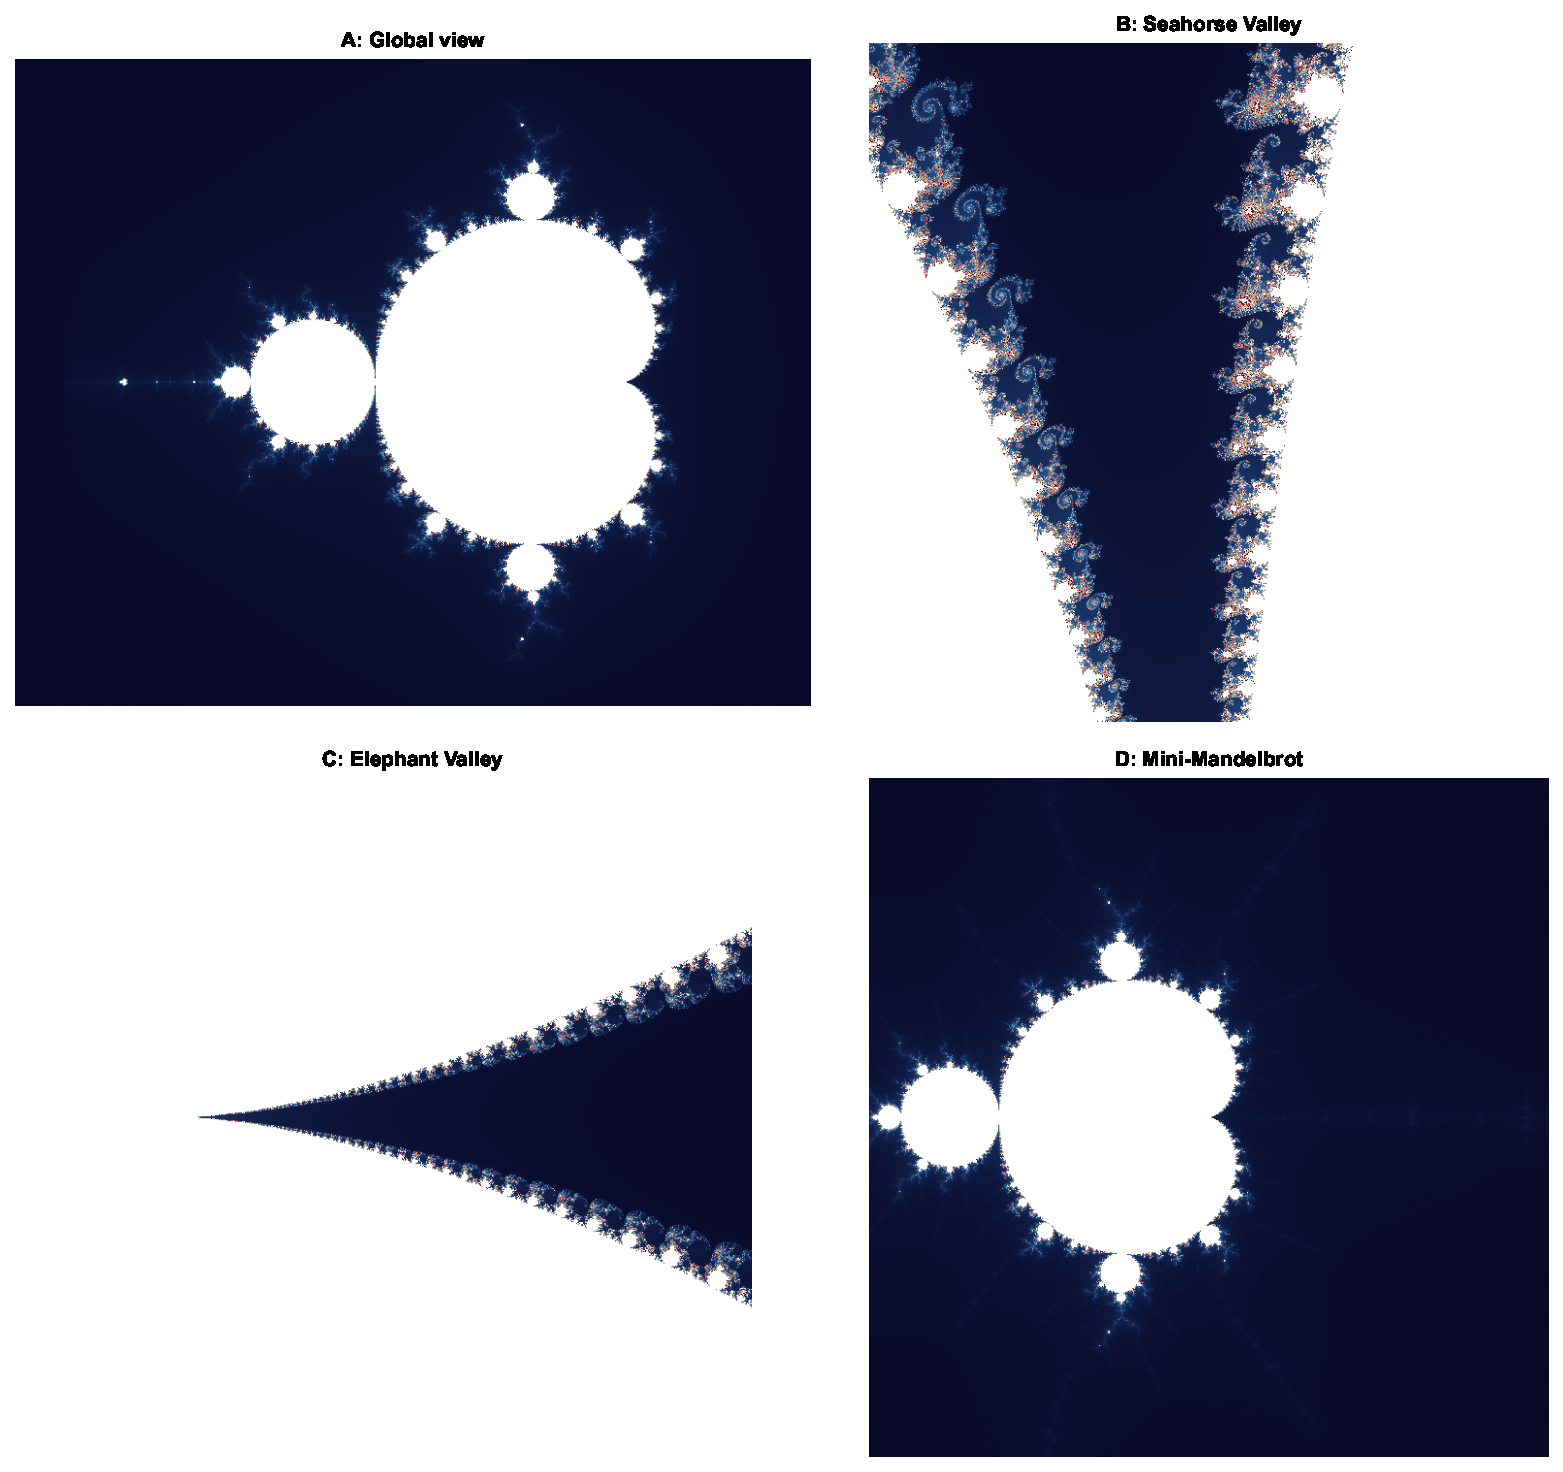
\includegraphics[width=\linewidth,height=4.5cm,keepaspectratio]{ch_fmh_mandelbrot_gallery.pdf}
\figql{SFM\_ch\_fmh\_fractals: mandelbrot\_gallery}{https://github.com/QuantLet/Stat_fin_markets/tree/master/Quantlets/SFM_ch_fmh}
\end{column}
\end{columns}
\end{cminipage}
\end{frame}

% TASK 4: eliminat "Mandelbrot vedere extinsă" (combinat în slide-ul precedent)

\slidelevel{MSc}
\begin{frame}[shrink=15]{Mulțimile Julia}
\begin{cminipage}{0.95\textwidth}
\begin{columns}[T]
\begin{column}{0.42\textwidth}
\begin{defn}[Mulțimea Julia $\mathcal{J}_c$]
Pentru un $c \in \mathbb{C}$ \textbf{fixat}, se consideră iterația:
\[
    z_{n+1} = z_n^2 + c, \quad z_0 \in \mathbb{C}
\]
Mulțimea Julia umplută este:
\[
    \mathcal{K}_c = \bigl\{ z \in \mathbb{C} : \{z_n\} \text{ mărginit} \bigr\}
\]
\textbf{Mulțimea Julia} $\mathcal{J}_c = \partial \mathcal{K}_c$ este \textit{frontiera}.
\end{defn}

\begin{itemize}\setlength{\itemsep}{0pt}
    \item \textbf{Teoremă fundamentală} (Fatou--Julia)
    \begin{itemize}\setlength{\itemsep}{0pt}
        \item $\mathcal{J}_c$ este \textbf{conexă} $\Leftrightarrow$ $c \in \mathcal{M}$
        \item $\mathcal{J}_c$ este \textbf{praf Cantor} $\Leftrightarrow$ $c \notin \mathcal{M}$
    \end{itemize}
    \item Mandelbrot este \textbf{dicționarul} mulțimilor Julia
    \item Estetic: spirale, dendrite, ,,iepuri Douady'', dragoni
\end{itemize}
\end{column}
\begin{column}{0.56\textwidth}
\centering
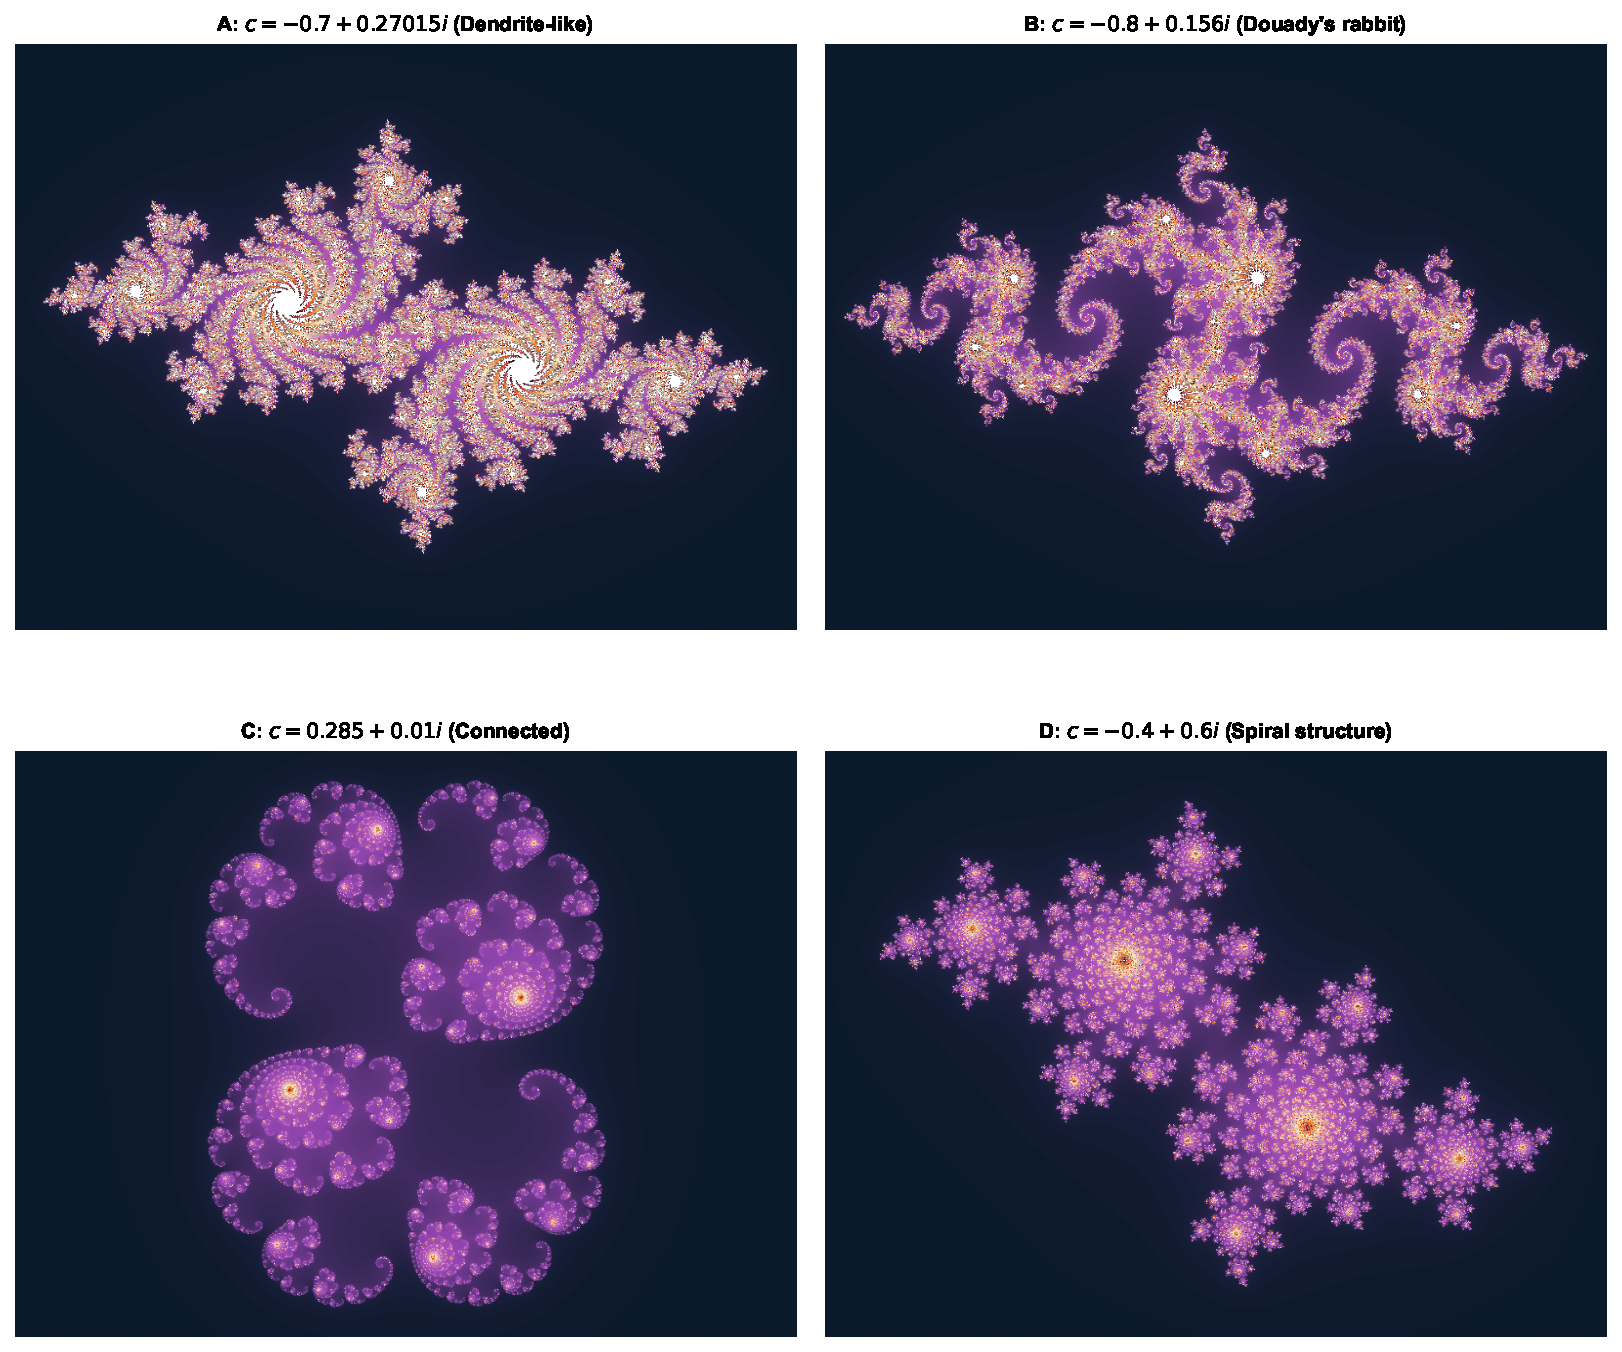
\includegraphics[width=\linewidth]{ch_fmh_julia_gallery.pdf}
\figql{SFM\_ch\_fmh\_fractals: julia\_gallery}{https://github.com/QuantLet/Stat_fin_markets/tree/master/Quantlets/SFM_ch_fmh}
\end{column}
\end{columns}
\end{cminipage}
\end{frame}

\slidelevel{MSc}
\begin{frame}[shrink=15]{Structura mulțimii Mandelbrot (Cardioid \& period bulbs)}
\begin{cminipage}{0.95\textwidth}
\begin{itemize}\setlength{\itemsep}{0pt}
    \item Componenta principală a $\mathcal{M}$ este \textbf{cardioida} (cardioid):
    \[
        \bigl\{ c \in \mathbb{C} : \exists\, z, \; z = z^2 + c, \; |2z| < 1 \bigr\}
    \]
    parametrizată ca $c(\theta) = \tfrac{1}{2}e^{i\theta}\bigl(1 - \tfrac{1}{2}e^{i\theta}\bigr)$
    \item \textbf{Period bulbs}: discuri atașate de cardioidă; fiecare disc $D_{p/q}$ atașat la unghiul $2\pi p/q$ corespunde unei \textbf{orbite periodice} de perioadă $q$ (ex.: $D_{1/3}$, $D_{1/2}$, $D_{2/5}$)
    \item \textbf{Punctul Misiurewicz}: $c$ pre-periodic, e.g., $c = -2, c = i$, dar $c = i \in \partial \mathcal{M}$
    \item \textbf{Filaments \& satellites}: structură fractală auto-similară pe frontieră
    \item \textbf{Rezultate teoretice celebre}:
    \begin{itemize}\setlength{\itemsep}{0pt}
        \item \textbf{Douady \& Hubbard (1982)}: $\mathcal{M}$ este \textbf{conexă}
        \item \textbf{Shishikura (1998)}: dimensiunea Hausdorff a $\partial \mathcal{M}$ este $D = 2$
        \item \textbf{Ipoteza MLC} (Mandelbrot Locally Connected): încă deschisă (problemă deschisă majoră în matematica modernă)
    \end{itemize}
    \item \textbf{Aplicații în finanțe}: distribuții care apar din iterații complexe ale unei aplicații dinamice (\textit{nonlinear dynamics in markets})
\end{itemize}
\end{cminipage}
\end{frame}

\slidelevel{MSc}
\begin{frame}[fragile, shrink=15]{Calculul mulțimii Mandelbrot: \textit{escape time algorithm}}
\begin{cminipage}{0.95\textwidth}
\begin{columns}[T]
\begin{column}{0.50\textwidth}
\begin{block}{Algoritm de bază (escape time)}
\begin{enumerate}\setlength{\itemsep}{0pt}
    \item Pentru fiecare pixel $c \in \mathbb{C}$:
    \item Inițializează $z_0 = 0$
    \item Iterează $z_{n+1} = z_n^2 + c$ până la $|z_n| > 2$ sau $n > N_{\max}$
    \item Dacă $|z_n| > 2$: $c \notin \mathcal{M}$, colorează după $n$
    \item Altfel: $c \in \mathcal{M}$ (interior, de obicei negru/alb)
\end{enumerate}
\end{block}

\begin{block}{Smooth coloring (continuous escape)}
\[
    \mu = n + 1 - \frac{\log \log |z_n|}{\log 2}
\]
elimină ,,benzile'' discrete și produce un gradient continuu.
\end{block}
\end{column}
\begin{column}{0.46\textwidth}
\begin{exampleblock}{Cod Python}
\scriptsize
\begin{verbatim}
def mandelbrot(c, max_iter=300):
    z = 0
    for n in range(max_iter):
        z = z*z + c
        if abs(z) > 2:
            return n + 1 - log(log(abs(z))) / log(2)
    return max_iter
\end{verbatim}
\end{exampleblock}

\begin{itemize}\setlength{\itemsep}{0pt}
    \item Complexitate: $O(W \cdot H \cdot N_{\max})$
    \item Vectorizare cu NumPy: $\sim 100\times$ accelerare
    \item GPU (CUDA): $\sim 10000\times$ accelerare
    \item Algoritmi avansați: \textit{distance estimator}, \textit{perturbation theory} (zoom $> 10^{15}$)
\end{itemize}
\end{column}
\end{columns}
\end{cminipage}
\end{frame}

% TASK 4: eliminat "Multibrot" (tangențial pentru SFM)

% TASK 4: eliminat "Burning Ship" (tangențial pentru SFM)

% TASK 4: eliminat slide "Fractalii Newton" (tangențial pentru SFM)

\slidelevel{MSc}
\begin{frame}[shrink=15]{Conexiunea Mandelbrot--Julia: dicționarul (Mandelbrot--Julia connection)}
\begin{cminipage}{0.95\textwidth}
\begin{thm}[Teorema fundamentală Julia--Fatou]
Pentru iterația $z_{n+1} = z_n^2 + c$:
\begin{itemize}\setlength{\itemsep}{0pt}
    \item Mulțimea Julia $\mathcal{J}_c$ este \textbf{conexă} dacă și numai dacă $c \in \mathcal{M}$
    \item $\mathcal{J}_c$ este \textbf{praf Cantor} (totally disconnected) dacă și numai dacă $c \notin \mathcal{M}$
\end{itemize}
\end{thm}
\begin{itemize}\setlength{\itemsep}{0pt}
    \item \textbf{Mandelbrot} $=$ \textbf{atlasul} mulțimilor Julia: fiecare punct $c \in \mathcal{M}$ corespunde unei mulțimi Julia conexe $\mathcal{J}_c$
    \item Forma \textit{locală} a $\mathcal{M}$ în jurul lui $c$ \textbf{aproximează} forma globală a $\mathcal{J}_c$
    \item \textbf{Implicare practică}: pentru a explora mulțimile Julia, navighezi prin $\mathcal{M}$:
    \begin{itemize}\setlength{\itemsep}{0pt}
        \item Cardioid $\Rightarrow$ Julia conexă, simplu conexă
        \item Period 2 bulb $\Rightarrow$ Julia formă de 8
        \item Period 3 bulb $\Rightarrow$ Julia formă de ,,iepure Douady''
        \item Filamente $\Rightarrow$ Julia tip dendrite
        \item Mini-Mandelbrot $\Rightarrow$ Julia mini-Mandelbrot-like
    \end{itemize}
    \item \textbf{Universalitate}: pattern-urile apar în multe sisteme dinamice (Feigenbaum, fluid turbulence, plasma physics)
\end{itemize}
\end{cminipage}
\end{frame}

% TASK 4: eliminat slide "Aplicații dincolo de matematică" (generalist, fără valoare directă pentru SFM)

%#############################################################################
\section{Exponentul Hurst}
%#############################################################################

\slidelevel{Y3}
\begin{frame}[shrink=20]{Harold Hurst și problema Nilului}
\begin{cminipage}{0.95\textwidth}
\begin{columns}[T]
\begin{column}{0.55\textwidth}
\begin{itemize}\setlength{\itemsep}{2pt}
    \item \textbf{Harold E. Hurst} (1880--1978), hidrolog britanic în Egipt
    \item Studiu al \textbf{nivelului anual al Nilului} (847--1284 d.Hr.) pentru proiectarea barajului Aswan
    \item Întrebare: ce capacitate trebuie să aibă un rezervor astfel încât niciodată să nu sece, indiferent de secetă?
    \item Hurst (1951): a observat că anii umezi tind să se grupeze, la fel și anii secetoși $\Rightarrow$ \textbf{dependență pe termen lung}
    \item A descoperit că ,,intervalul rescalat'' $R/S$ scalează ca $n^H$ cu
    \[
        H \approx 0{,}73
    \]
    \item Mult mai mare decât $H = 0{,}5$ așteptat pentru observații independente!
    \item \textbf{,,Efectul Joseph''} (Mandelbrot, 1968) --- după biblicii ,,7 ani buni urmați de 7 ani răi''
\end{itemize}
\end{column}
\begin{column}{0.42\textwidth}
\centering
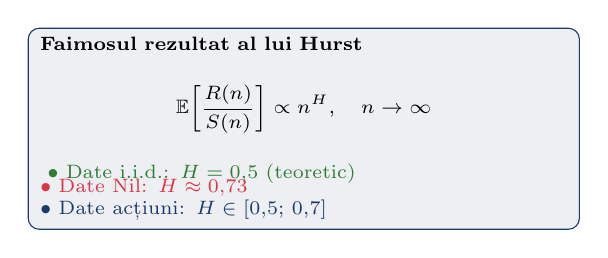
\begin{tikzpicture}[every node/.style={font=\scriptsize, align=center}]
\node[draw=MainBlue, fill=MainBlue!8, rounded corners=4pt,
      minimum width=7cm, minimum height=2.0cm, align=left, text width=6.7cm] (n1) {%
\textbf{Faimosul rezultat al lui Hurst}
\vspace{0.05cm}
\[
    \E\!\left[\frac{R(n)}{S(n)}\right] \propto n^H, \quad n \to \infty
\]
\vspace{-0.1cm}
\textcolor{Forest}{$\bullet$ Date i.i.d.: $H = 0{,}5$ (teoretic)} \\
\textcolor{Crimson}{$\bullet$ Date Nil: $H \approx 0{,}73$} \\
\textcolor{MainBlue}{$\bullet$ Date acțiuni: $H \in [0{,}5;\, 0{,}7]$}
};
\end{tikzpicture}

\vspace{0.3cm}

\begin{block}{Mandelbrot \& Wallis (1969)}
\begin{itemize}\setlength{\itemsep}{0pt}
    \item \scriptsize \textit{,,Hurst este la geometria fractală ce este Bachelier la mersul aleator''}
    \item \scriptsize \textit{,,Pionierul unei lumi noi''}
\end{itemize}
\end{block}
\end{column}
\end{columns}
\end{cminipage}
\end{frame}

\slidelevel{Y3}
\begin{frame}[shrink=20]{Definiția exponentului Hurst}
\begin{cminipage}{0.95\textwidth}
\begin{defn}[Exponentul Hurst]
\textbf{Exponentul Hurst} $H \in (0, 1)$ caracterizează structura de dependență pe termen lung a unei serii de timp:
\begin{itemize}\setlength{\itemsep}{0pt}
    \item $H = 0{,}5$: \textbf{mers aleator} (fără memorie); incremenți independenți; consistent cu EMH
    \item $H > 0{,}5$: \textbf{persistent} / \textit{trending}; autocorelație pozitivă pe termen lung
    \item $H < 0{,}5$: \textbf{anti-persistent} / mean-reverting; autocorelație negativă pe termen lung
\end{itemize}
\end{defn}

\begin{columns}[T]
\begin{column}{0.50\textwidth}
\begin{itemize}\setlength{\itemsep}{0pt}
    \item Pentru un proces autosimilar, varianța mediei pe ferestre de mărime $n$ scalează ca:
    \[
        \Var\!\left(\frac{1}{n}\sum_{i=1}^n r_i\right) \sim C \cdot n^{2H - 2}, \quad n \to \infty
    \]
    \item Când $H > 0{,}5$, varianța descrește \textbf{mai lent} decât $n^{-1}$ $\Rightarrow$ legea numerelor mari nu se aplică la rata uzuală
    \item \textbf{Memoria lungă}: autocorelațiile decad ca $\rho(k) \sim C \, k^{2H-2}$ (decadere hiperbolică, nu exponențială)
\end{itemize}
\end{column}
\begin{column}{0.46\textwidth}
\centering
\renewcommand{\arraystretch}{1.3}
\begin{tabular}{ccl}
\toprule
$H$ & $D$ & \textbf{Interpretare} \\
\midrule
$0{,}1$ & $1{,}9$ & Foarte anti-persistent \\
$0{,}3$ & $1{,}7$ & Mean-reverting \\
$0{,}5$ & $1{,}5$ & Mers aleator (Brown) \\
$0{,}7$ & $1{,}3$ & Persistent moderat \\
$0{,}9$ & $1{,}1$ & Foarte persistent \\
\bottomrule
\end{tabular}

\vspace{0.3cm}

\begin{itemize}\setlength{\itemsep}{0pt}
    \item \small Relația Hurst--dimensiune fractală: $\;\boxed{\; D = 2 - H \;}\;$
\end{itemize}
\end{column}
\end{columns}
\end{cminipage}
\end{frame}

\slidelevel{Y3}
\begin{frame}[shrink=15]{Efectul Joseph și efectul Noah (Joseph effect \& Noah effect)}
\begin{cminipage}{0.95\textwidth}
\begin{columns}[T]
\begin{column}{0.50\textwidth}
\begin{block}{Efectul Joseph (long memory / persistence)}
\begin{itemize}\setlength{\itemsep}{0pt}
    \item Mandelbrot (1968): biblicii ,,7 ani buni urmați de 7 ani răi'' (Iosif și interpretarea visului faraonului)
    \item Cuantifică \textbf{persistența pe termen lung}: trenduri continuă
    \item Capturat de exponentul Hurst: $H > 0{,}5$
    \item Modelat de \textbf{fBm} și \textbf{ARFIMA}
    \item Exemplu: niveluri ale Nilului 847--1284 d.Hr.
\end{itemize}
\end{block}
\end{column}
\begin{column}{0.46\textwidth}
\begin{alertblock}{Efectul Noah (heavy tails / discontinuity)}
\begin{itemize}\setlength{\itemsep}{0pt}
    \item Mandelbrot (1968): potopul biblic --- evenimente catastrofale, discontinue
    \item Cuantifică \textbf{cozile grele}: salturi mari sunt comune
    \item Capturat de \textbf{exponentul $\alpha$ Lévy} ($\alpha < 2$)
    \item Modelat de \textbf{procese Lévy stabile} și \textbf{procese de salt}
    \item Exemplu: Black Monday 1987, COVID-19
\end{itemize}
\end{alertblock}
\end{column}
\end{columns}

\vspace{0.3cm}

\begin{exampleblock}{Combinarea celor două efecte}
\begin{itemize}\setlength{\itemsep}{0pt}
    \item \textbf{Multifractal stable Lévy motion} (Mandelbrot, 1997): permite simultan memorie lungă (Joseph) și salturi (Noah)
    \item Modelează \textbf{toate stilurile faptelor stilizate} ale piețelor
    \item Generalizare a fBm $\Rightarrow$ \textbf{linear fractional stable motion} (LFSM)
\end{itemize}
\end{exampleblock}
\end{cminipage}
\end{frame}

\slidelevel{MSc}
\begin{frame}[shrink=15]{Hurst în alte domenii (Hurst exponent in other fields)}
\begin{cminipage}{0.95\textwidth}
\renewcommand{\arraystretch}{1.25}
\begin{center}
\small
\begin{tabular}{lll}
\toprule
\textbf{Domeniu} & \textbf{Serie} & \textbf{$\hat{H}$ tipic} \\
\midrule
Hidrologie & Niveluri Nil (847--1284 d.Hr.) & $\approx 0{,}73$ \\
Climatologie & Temperaturi anuale globale (1850--2020) & $0{,}65$--$0{,}90$ \\
Cardiologie & Inter-bătăi cardiace (subiect sănătos) & $\approx 1{,}0$ ($1/f$ noise) \\
Cardiologie & Insuficiență cardiacă & $\approx 0{,}5$ (pierderea complexității!) \\
Neuroștiințe & Activitate EEG & $0{,}6$--$0{,}8$ \\
Geofizică & Cutremure (magnitudine \& timp) & Multifractal \\
Trafic Internet & Pachete pe rețea & $\approx 0{,}9$ (long memory!) \\
Astronomie & Distribuția galaxiilor & Multifractal $D \in [1{,}2, 2{,}0]$ \\
Lingvistică & Frecvența cuvintelor (Zipf) & Multifractal \\
Finanțe & Indici de acțiuni & $0{,}5$--$0{,}65$ \\
Finanțe & Cripto (BTC, ETH) & $0{,}50$--$0{,}75$ \\
Finanțe & Forex (EUR/USD, lichid) & $\approx 0{,}51$ \\
\bottomrule
\end{tabular}
\end{center}
\vspace{0.15cm}
\begin{itemize}\setlength{\itemsep}{0pt}
    \item \textbf{Universalitate}: ,,$1/f$ noise'' apare în zeci de sisteme complexe
    \item \textbf{Sănătatea} unui sistem complex $\Leftrightarrow$ menținerea complexității fractale
    \item \textbf{Aplicație}: dispariția fractalității poate fi un \textbf{semnal de avertizare} (degradare cardiacă, criză financiară, instabilitate climatică)
\end{itemize}
\end{cminipage}
\end{frame}

\slidelevel{Y3}
% TASK 3: split slide "Proprietăți Hurst" în 2 frame-uri
\begin{frame}[shrink=10]{Hurst --- proprietăți de bază (Hurst basic properties)}
\begin{cminipage}{0.95\textwidth}
\begin{itemize}\setlength{\itemsep}{2pt}
    \item \textbf{Domeniu}: $H \in (0, 1)$ pentru fBm
    \item \textbf{Dimensiunea fractală a graficului}:
    \[
        D = 2 - H \quad \text{(graficul prețului în plan)}
    \]
    \item \textbf{Varianța increment}:
    \[
        \E[(B_H(t+\tau) - B_H(t))^2] = \tau^{2H}
    \]
    \item \textbf{Autocorelația incrementelor (fGn)}:
    \[
        \rho(k) \sim H(2H-1) k^{2H-2}, \quad k \to \infty
    \]
\end{itemize}
\end{cminipage}
\end{frame}

\slidelevel{MSc}
\begin{frame}[shrink=10]{Hurst --- extensii și conexiuni (Hurst extensions \& connections)}
\begin{cminipage}{0.95\textwidth}
\begin{itemize}\setlength{\itemsep}{2pt}
    \item \textbf{Densitatea spectrală}:
    \[
        S(\omega) \sim |\omega|^{1-2H}, \quad \omega \to 0
    \]
    \item \textbf{Conexiunea cu ARFIMA}: $d = H - 1/2 \in (-1/2, 1/2)$
    \item \textbf{Conexiunea cu DFA exponent} $\alpha$: $\alpha = H$ pentru fBm/fGn integrat
    \item \textbf{Robustețe}: $\hat{H}$ robust la transformări monotone și la zgomot aditiv mic
\end{itemize}
\end{cminipage}
\end{frame}

%#############################################################################
\section{Analiza R/S}
%#############################################################################

\slidelevel{MSc}
\begin{frame}[shrink=20]{Analiza R/S (Rescaled Range)}
\begin{cminipage}{0.95\textwidth}
\begin{itemize}\setlength{\itemsep}{0pt}
    \item Metoda \textbf{clasică} pentru estimarea lui $H$ (Hurst, 1951; Mandelbrot \& Wallis, 1969)
    \item \textbf{Algoritm}: pentru o serie $\{x_1, \ldots, x_N\}$
    \begin{enumerate}\setlength{\itemsep}{0pt}
        \item Împarte seria în blocuri non-suprapuse de mărime $n$
        \item Pentru fiecare bloc $\{x_1, \ldots, x_n\}$, calculează media: $\bar{x}_n = \frac{1}{n}\sum_{i=1}^n x_i$
        \item Calculează \textbf{deviațiile cumulate}: $Y_k = \sum_{i=1}^k (x_i - \bar{x}_n)$, \quad $k = 1, \ldots, n$
        \item Calculează \textbf{intervalul} (range): $R(n) = \max_{k} Y_k - \min_{k} Y_k$
        \item Calculează \textbf{deviația standard}: $S(n) = \sqrt{\frac{1}{n}\sum_{i=1}^n (x_i - \bar{x}_n)^2}$
        \item \textbf{Intervalul rescalat}: $(R/S)_n = R(n) / S(n)$
    \end{enumerate}
    \item \textbf{Legea Hurst}: $\E\!\left[R(n)/S(n)\right] \propto n^H$ când $n \to \infty$
    \item Estimare prin regresie OLS:
    \[
        \log\!\left(\frac{R(n)}{S(n)}\right) = \hat{H} \cdot \log(n) + c + \text{eroare}
    \]
    \item \textbf{Limitări}: sensibilă la dependență pe termen scurt și non-staționaritate. Lo (1991) a propus statistica R/S \textbf{modificată}, care corectează autocorelațiile pe termen scurt
\end{itemize}
\end{cminipage}
\end{frame}

\slidelevel{MSc}
\begin{frame}[fragile, shrink=15]{R/S în Python}
\begin{cminipage}{0.95\textwidth}
\begin{lstlisting}
import numpy as np
from scipy import stats

def rs_analysis(x, min_n=10, max_n=None):
    """Estimeaza exponentul Hurst prin analiza R/S."""
    x = np.asarray(x, dtype=float)
    T = len(x)
    if max_n is None:
        max_n = T // 4
    ns = np.unique(np.logspace(np.log10(min_n), np.log10(max_n), 40).astype(int))
    rs_vals = []
    for n in ns:
        n_blocks = T // n
        rs_block = []
        for b in range(n_blocks):
            block = x[b*n : (b+1)*n]
            cumdev = np.cumsum(block - block.mean())
            R = cumdev.max() - cumdev.min()
            S = block.std(ddof=0)
            if S > 1e-15:
                rs_block.append(R / S)
        rs_vals.append(np.mean(rs_block) if rs_block else np.nan)
    log_n = np.log(ns); log_rs = np.log(rs_vals)
    H, _, _, _, _ = stats.linregress(log_n, log_rs)
    return H, ns, rs_vals
\end{lstlisting}
\end{cminipage}
\quantlet{SFM\_ch14\_fractal\_hurst}{https://github.com/QuantLet/Stat_fin_markets/tree/master/Quantlets/SFM_ch14}
\end{frame}

\slidelevel{MSc}
\begin{frame}[shrink=20]{Exemplu pas-cu-pas: R/S pe o serie scurtă}
\begin{cminipage}{0.95\textwidth}
\begin{exampleblock}{Date: 8 randamente (\%)}
\begin{itemize}\setlength{\itemsep}{0pt}
    \item Seria: $\{0{,}5;\, -0{,}3;\, 0{,}8;\, -0{,}2;\, 0{,}6;\, -0{,}1;\, 0{,}4;\, -0{,}7\}$
    \item Mărimea blocului: $n = 8$
\end{itemize}
\end{exampleblock}

\begin{itemize}\setlength{\itemsep}{0pt}
    \item Pas 1: media $\bar{x} = (0{,}5 - 0{,}3 + 0{,}8 - 0{,}2 + 0{,}6 - 0{,}1 + 0{,}4 - 0{,}7)/8 = 0{,}125$
    \item Pas 2: deviații $x_i - \bar{x}$:\\
    $\{0{,}375;\, -0{,}425;\, 0{,}675;\, -0{,}325;\, 0{,}475;\, -0{,}225;\, 0{,}275;\, -0{,}825\}$
    \item Pas 3: cumulate $Y_k = \sum_{i=1}^k(x_i - \bar{x})$:\\
    $\{0{,}375;\, -0{,}050;\, 0{,}625;\, 0{,}300;\, 0{,}775;\, 0{,}550;\, 0{,}825;\, 0\}$
    \item Pas 4: range $R = \max(Y) - \min(Y) = 0{,}825 - (-0{,}050) = 0{,}875$
    \item Pas 5: deviația standard $S = \sqrt{\frac{1}{8}\sum(x_i - \bar{x})^2}$
    \[
        \frac{1}{8}\bigl(0{,}141 + 0{,}181 + 0{,}456 + 0{,}106 + 0{,}226 + 0{,}051 + 0{,}076 + 0{,}681\bigr) = 0{,}240, \quad S = 0{,}490
    \]
    \item Pas 6: $R/S = 0{,}875 / 0{,}490 = 1{,}786$
    \item Repetă pentru $n = 4, 8, 16, \ldots$ și fă regresie OLS pentru a găsi $\hat{H}$
\end{itemize}
\end{cminipage}
\end{frame}

\slidelevel{PhD}
\begin{frame}[shrink=15]{Statistica R/S modificată Lo (1991) (Modified R/S)}
\begin{cminipage}{0.95\textwidth}
\begin{itemize}\setlength{\itemsep}{0pt}
    \item \textbf{Critica} R/S clasică: confundă \textbf{memoria pe termen lung} cu \textbf{memoria pe termen scurt}
    \item Andrew Lo (1991): propune înlocuirea $S^2$ cu o \textbf{varianță Newey--West} care corectează autocorelațiile pe termen scurt
    \item Statistica modificată:
    \[
        Q_n = \frac{R(n)}{\sigma_n(q)}
    \]
    unde:
    \[
        \sigma_n^2(q) = \hat{\gamma}_0 + 2 \sum_{j=1}^{q} w_j(q)\, \hat{\gamma}_j, \quad w_j(q) = 1 - \frac{j}{q+1}
    \]
    cu $\hat{\gamma}_j$ autocovarianța la lag $j$ și $w_j$ ponderi Bartlett
    \item \textbf{Distribuția asimptotică} sub $H_0: H = 1/2$:
    \[
        \frac{Q_n}{\sqrt{n}} \xrightarrow{d} V \quad \text{(Lo, 1991, Tabel I)}
    \]
    \item Test pentru $H = 0{,}5$: respinge dacă $Q_n / \sqrt{n} \notin [0{,}809, 1{,}862]$ la $\alpha = 5\%$
    \item \textbf{Aplicare}: Lo a respins memoria lungă pentru indici US (1991), dar studii ulterioare (Greene \& Fielitz 1977) au găsit memorie lungă pe sub-perioade
\end{itemize}
\end{cminipage}
\end{frame}

\slidelevel{PhD}
\begin{frame}[shrink=15]{Variance ratio (VR) test și conexiunea cu Hurst}
\begin{cminipage}{0.95\textwidth}
\begin{itemize}\setlength{\itemsep}{0pt}
    \item \textbf{Variance Ratio test} (Lo \& MacKinlay, 1988): test direct pentru \textbf{mers aleator} (random walk)
    \item Statistica VR pentru orizont $q$:
    \[
        VR(q) = \frac{\Var(r_t(q))}{q \cdot \Var(r_t(1))}
    \]
    unde $r_t(q) = r_t + r_{t-1} + \cdots + r_{t-q+1}$
    \item Sub mers aleator: $VR(q) = 1$
    \item \textbf{Conexiunea cu Hurst}: dacă $r_t \sim$ fGn cu exponent $H$:
    \[
        VR(q) \sim q^{2H - 1}
    \]
    \item \textbf{Estimator Hurst pe baza VR}:
    \[
        \hat{H} = \frac{1}{2}\bigl(1 + \frac{\log VR(q)}{\log q}\bigr)
    \]
    \item \textbf{Avantaje}: distribuția asimptotică e gaussiană, intervalele de încredere ușor de construit
    \item \textbf{Test multiple-horizon} (Chow-Denning, 1993): combină mai multe orizonturi $q$ într-un test unic
    \item \textbf{Quantleturi disponibile}: \texttt{SFM\_ch4\_vr\_with\_ci}, \texttt{SFM\_ch4\_mv\_test} (Cap.~4)
\end{itemize}
\end{cminipage}
\end{frame}

\slidelevel{PhD}
\begin{frame}[shrink=15]{Bias și varianța estimatorilor Hurst}
\begin{cminipage}{0.95\textwidth}
\renewcommand{\arraystretch}{1.25}
\begin{center}
\small
\begin{tabular}{llll}
\toprule
\textbf{Estimator} & \textbf{Bias} & \textbf{Varianță} & \textbf{Robust la non-staționaritate} \\
\midrule
R/S clasic (Hurst, 1951) & Mare ($+$) la $H \approx 0{,}5$ & Mediu & Nu \\
R/S modificat (Lo, 1991) & Mic & Mare & Parțial \\
DFA-1 (Peng, 1994) & Mic & Mediu & Da (trenduri liniare) \\
DFA-2, DFA-3 & Foarte mic & Mediu & Da (trenduri polinomiale) \\
Variance ratio (Lo-MacKinlay) & Mic & Mic & Nu \\
Periodogramă (GPH, 1983) & Mic la $H$ aproape de $0{,}5$ & Mare & Nu \\
Wavelet (WTMM) & Foarte mic & Mic & Da (cea mai bună!) \\
Whittle (semi-parametric) & Mic & Foarte mic & Da \\
\bottomrule
\end{tabular}
\end{center}
\vspace{0.2cm}
\begin{itemize}\setlength{\itemsep}{0pt}
    \item \textbf{Recomandare}: folosiți \textbf{mai multe estimatori} și verificați coerența
    \item Pentru piețe financiare reale: combinați R/S, DFA, VR și wavelets
    \item \textbf{Studii Monte Carlo} arată că diferențele între estimatori pot fi $\pm 0{,}05$ la $H$ adevărat
\end{itemize}
\end{cminipage}
\end{frame}

%#############################################################################
\section{DFA (Detrended Fluctuation Analysis)}
%#############################################################################

\slidelevel{MSc}
\begin{frame}[shrink=20]{DFA: Analiza Fluctuațiilor Detrendate}
\begin{cminipage}{0.95\textwidth}
\begin{itemize}\setlength{\itemsep}{0pt}
    \item \textbf{DFA} introdusă de Peng et al. (1994), inițial pentru analiza ADN-ului
    \item \textbf{Avantaje față de R/S}: robustă la non-staționaritate și trenduri polinomiale
    \item \textbf{Algoritm}: pentru o serie $\{x_1, \ldots, x_N\}$
    \begin{enumerate}\setlength{\itemsep}{0pt}
        \item Calculează \textbf{seria integrată} (profilul): $Y_k = \sum_{i=1}^k (x_i - \bar{x})$
        \item Împarte $\{Y_k\}$ în segmente non-suprapuse de mărime $n$
        \item În fiecare segment, ajustează un polinom $\hat{Y}_k^{(m)}$ de ordin $m$ (DFA-1: linear; DFA-2: pătratic)
        \item Calculează \textbf{funcția de fluctuație}:
        \[
            F(n) = \sqrt{\frac{1}{N}\sum_{k=1}^{N} \left(Y_k - \hat{Y}_k^{(m)}\right)^2}
        \]
        \item Legea de scalare: $F(n) \propto n^H$
    \end{enumerate}
    \item Estimează $\hat{H}$ din panta $\log F(n)$ vs $\log n$
    \item \textbf{Interpretare}:
    \begin{itemize}\setlength{\itemsep}{0pt}
        \item $H < 0{,}5$: anti-persistent
        \item $H = 0{,}5$: necorelat (zgomot alb)
        \item $0{,}5 < H < 1$: persistent / memorie lungă
        \item $H \approx 1$: zgomot $1/f$ (specific sistemelor critice)
        \item $H > 1$: non-staționar, divergent
    \end{itemize}
\end{itemize}
\end{cminipage}
\end{frame}

\slidelevel{MSc}
\begin{frame}[shrink=20]{Aplicație R/S și DFA pe SPY, BTC, EUR/USD}
\begin{cminipage}{0.96\textwidth}
\centering
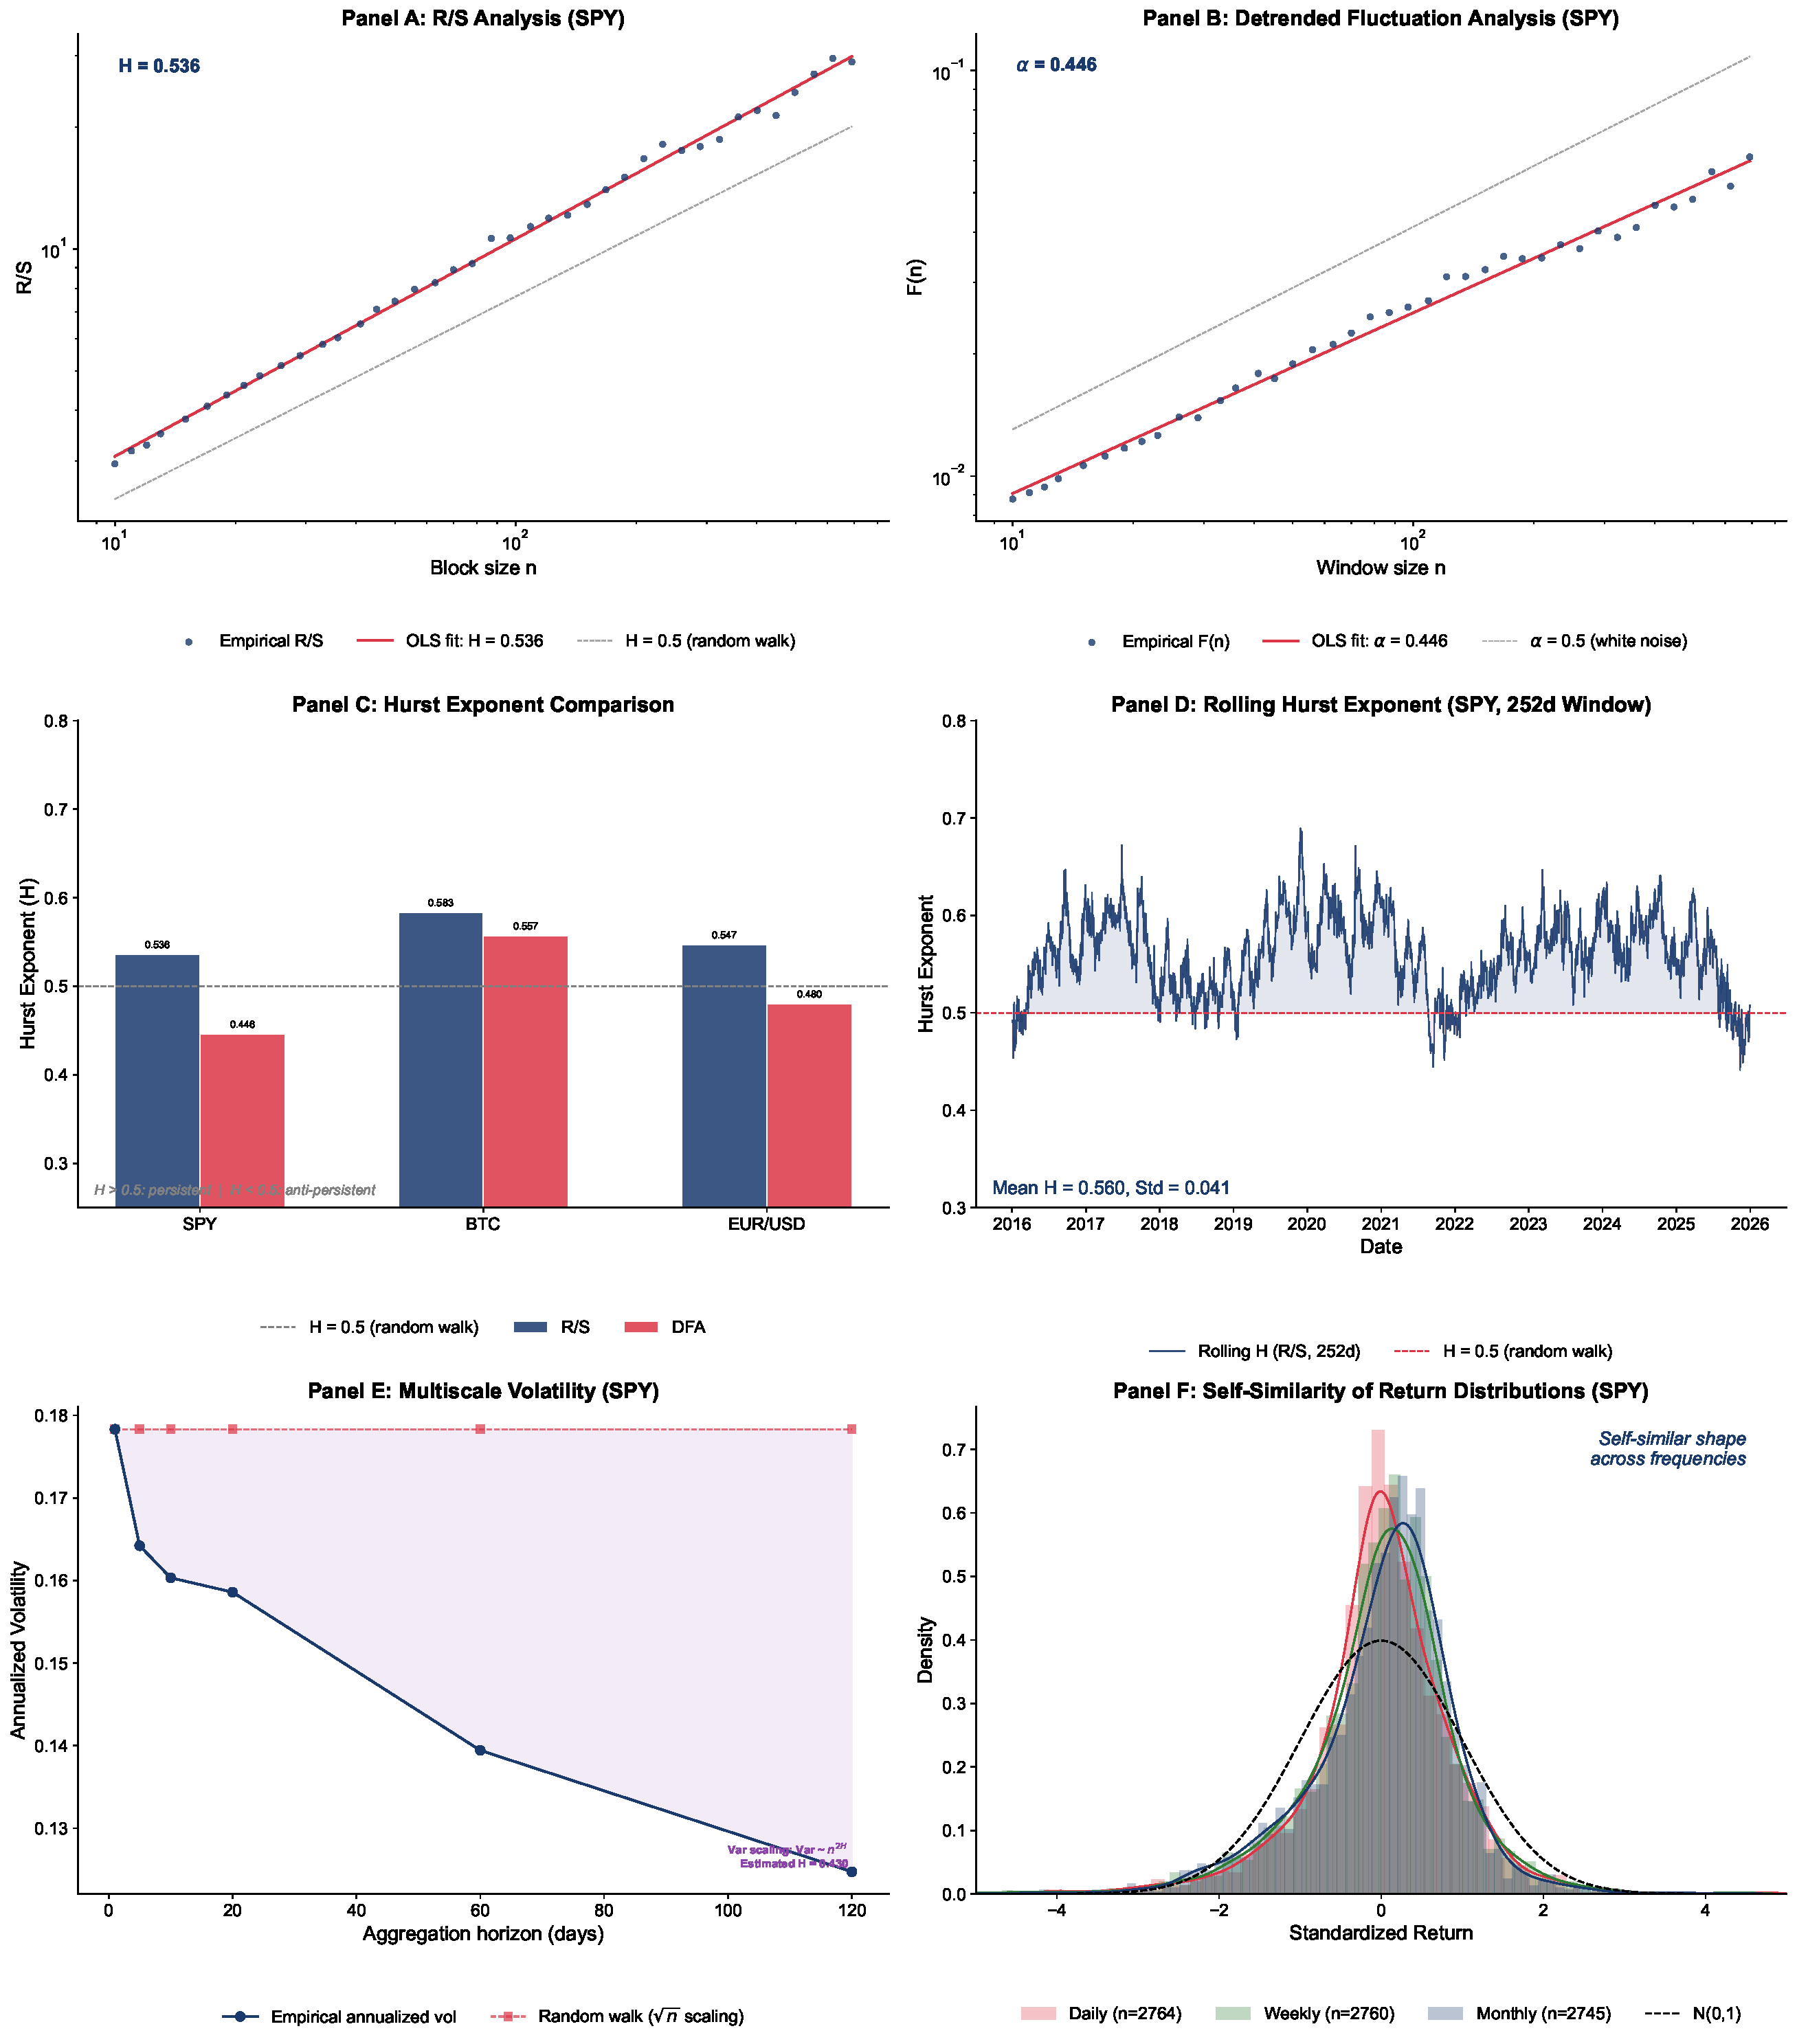
\includegraphics[height=6.0cm]{ch14_fractal_hurst.pdf}\\[2pt]
{\scriptsize\textcolor{MediumGray}{\textit{Panel A: scalarea R/S pentru SPY (slope $\approx H$). Panel B: DFA pe SPY. Panel C: comparație $H$ între active. Panel D: Hurst rolling. Panel E: scalarea volatilității multi-orizont. Panel F: autosimilaritate distribuțională.}}}
\end{cminipage}
\quantlet{SFM\_ch14\_fractal\_hurst}{https://github.com/QuantLet/Stat_fin_markets/tree/master/Quantlets/SFM_ch14}
\end{frame}

\slidelevel{PhD}
\begin{frame}[shrink=15]{DFA-1, DFA-2, DFA-3 (polynomial detrending order)}
\begin{cminipage}{0.95\textwidth}
\begin{itemize}\setlength{\itemsep}{0pt}
    \item \textbf{DFA-$m$}: ordinul polinomului folosit pentru detrendare
    \begin{itemize}\setlength{\itemsep}{0pt}
        \item DFA-1: detrendare \textbf{liniară} (linear) — elimină trenduri liniare
        \item DFA-2: detrendare \textbf{pătratică} (quadratic) — elimină trenduri pătratice
        \item DFA-3: detrendare \textbf{cubică} (cubic) — elimină trenduri cubice
    \end{itemize}
    \item \textbf{Regulă generală}: DFA-$m$ elimină trenduri polinomiale de grad $\leq m$
    \item \textbf{Limita DFA}: pentru DFA-$m$, exponentul $\alpha$ valid în:
    \[
        \alpha \in (0, m+1)
    \]
    \item \textbf{Crossover scaling}: dacă seria are mai multe regimuri (e.g., scurt vs lung), DFA poate detecta multiple pante:
    \[
        F(n) \sim n^{\alpha_1} \text{ pentru } n < n^* \quad \text{și} \quad F(n) \sim n^{\alpha_2} \text{ pentru } n > n^*
    \]
    \item \textbf{Recomandare practică}:
    \begin{itemize}\setlength{\itemsep}{0pt}
        \item Pentru randamente bursiere: DFA-1 sau DFA-2 (trenduri puține)
        \item Pentru prețuri (non-staționare): DFA-2 sau DFA-3
        \item Pentru date cu sezonalitate: \textbf{Centered Moving Average DFA} (CMA-DFA)
    \end{itemize}
\end{itemize}
\end{cminipage}
\end{frame}

\slidelevel{PhD}
\begin{frame}[shrink=15]{Multifractal DFA (MFDFA, Kantelhardt et al. 2002)}
\begin{cminipage}{0.95\textwidth}
\begin{itemize}\setlength{\itemsep}{0pt}
    \item Generalizarea DFA pentru \textbf{semnale multifractale}
    \item \textbf{Algoritm MFDFA}:
    \begin{enumerate}\setlength{\itemsep}{0pt}
        \item Calculează profilul $Y_k = \sum_{i=1}^k(x_i - \bar{x})$
        \item Împarte în segmente non-suprapuse de mărime $n$
        \item Detrendare polinomială locală în fiecare segment
        \item Funcția de fluctuație $q$-dependentă:
        \[
            F_q(n) = \left\{ \frac{1}{2 N_s} \sum_{v=1}^{2 N_s} \bigl[F^2(v, n)\bigr]^{q/2} \right\}^{1/q}
        \]
        \item Pentru fiecare $q$: $F_q(n) \sim n^{h(q)}$
    \end{enumerate}
    \item \textbf{Funcția $h(q)$}: \textbf{exponentul Hurst generalizat} (generalized Hurst exponent)
    \begin{itemize}\setlength{\itemsep}{0pt}
        \item $h(2) =$ Hurst clasic
        \item $h(q)$ \textbf{constant} în $q$ $\Rightarrow$ \textbf{monofractal}
        \item $h(q)$ \textbf{descrescător} în $q$ $\Rightarrow$ \textbf{multifractal}
    \end{itemize}
    \item Conexiunea cu spectrul multifractal:
    \[
        \tau(q) = q \cdot h(q) - 1, \qquad \alpha = h(q) + q \cdot h'(q), \qquad f(\alpha) = q[\alpha - h(q)] + 1
    \]
    \item Pachet Python: \texttt{MFDFA} (Gomes-Silva, 2021)
\end{itemize}
\end{cminipage}
\end{frame}

\slidelevel{PhD}
\begin{frame}[shrink=15]{Wavelet methods (WTMM, wavelet leaders)}
\begin{cminipage}{0.95\textwidth}
\begin{itemize}\setlength{\itemsep}{0pt}
    \item \textbf{Wavelet Transform Modulus Maxima} (WTMM, Muzy, Bacry, Arneodo 1991)
    \item Idee: descompunere în wavelets (e.g., Daubechies, Mexican Hat) la \textbf{multiple scale}:
    \[
        T_\psi[X](a, t) = \int X(t') \psi^*\!\left(\frac{t' - t}{a}\right) dt'
    \]
    \item Funcția de partiție generalizată:
    \[
        Z(q, a) = \sum_{(t_i, a) \in \mathcal{L}(a)} |T_\psi[X](t_i, a)|^q
    \]
    unde $\mathcal{L}(a)$ sunt liniile de maxim local
    \item Scaling: $Z(q, a) \sim a^{\tau(q)}$
    \item \textbf{Avantaje WTMM}:
    \begin{itemize}\setlength{\itemsep}{0pt}
        \item Robust la trenduri (mai bun decât DFA)
        \item Multiscale natural
        \item Localizare tempo-frecvență
    \end{itemize}
    \item \textbf{Wavelet leaders} (Jaffard, Lashermes, Abry, 2007): variantă mai stabilă numeric
    \item Aplicate cu succes pe: turbulență, semnale fiziologice, randamente bursiere intraday
\end{itemize}
\end{cminipage}
\end{frame}

\slidelevel{MSc}
\begin{frame}[shrink=15]{Comparație metode de estimare (estimator comparison)}
\begin{cminipage}{0.95\textwidth}
\renewcommand{\arraystretch}{1.25}
\begin{center}
\small
\begin{tabular}{llll}
\toprule
\textbf{Metodă} & \textbf{Tip semnal} & \textbf{Pachet Python} & \textbf{Recomandare} \\
\midrule
R/S clasic & Staționar & \texttt{nolds.hurst\_rs} & Educațional, simplu \\
R/S modificat (Lo) & Staționar + corel. scurte & \texttt{statsmodels} & Test formal $H=0{,}5$ \\
DFA-1 & Trenduri liniare & \texttt{nolds.dfa} & Standard pentru randamente \\
DFA-2/3 & Trenduri polinomiale & \texttt{nolds.dfa(order=2)} & Pentru prețuri non-staționare \\
MFDFA & Multifractal & \texttt{MFDFA} (PyPI) & Pentru spectru complet \\
GPH (1983) & Staționar & \texttt{arch} & Periodogramă \\
Whittle & Staționar & implementare proprie & Cel mai precis (semi-param) \\
Wavelet (WTMM) & Multifractal, robust & \texttt{pywt} + custom & Cea mai bună acuratețe \\
\bottomrule
\end{tabular}
\end{center}
\vspace{0.2cm}
\begin{exampleblock}{Combo recomandat pentru randamente bursiere}
\begin{itemize}\setlength{\itemsep}{0pt}
    \item \textbf{DFA-1} ca estimator principal $\hat{H}$
    \item \textbf{Variance ratio} (Lo--MacKinlay) ca test formal $H_0: H = 0{,}5$
    \item \textbf{MFDFA} pentru spectrul multifractal (dacă disponibilă putere de calcul)
    \item \textbf{R/S modificat} ca \textit{robustness check}
\end{itemize}
\end{exampleblock}
\end{cminipage}
\end{frame}

% TASK 7: quiz formativ §7 DFA
\slidelevel{MSc}
\begin{frame}{Test rapid: §7 DFA (quiz DFA)}
\begin{cminipage}{0.95\textwidth}
\begin{enumerate}\setlength{\itemsep}{2pt}
    \item<1-> Pentru o serie cu $\hat{H} = 0{,}48$ stabil, interpretarea este:
    \begin{itemize}\setlength{\itemsep}{0pt}
        \item A) Persistent
        \item B) Aproximativ random walk \onslide<2->{\textbf{← răspuns}}
        \item C) Strong anti-persistence
    \end{itemize}
    \item<3-> Când alegi DFA-2 sau DFA-3 vs DFA-1?
    \begin{itemize}\setlength{\itemsep}{0pt}
        \item A) Mereu DFA-1 (cel mai rapid)
        \item B) Când seria are trenduri non-staționare \onslide<4->{\textbf{← răspuns}}
        \item C) Când seria e staționară
    \end{itemize}
    \item<5-> Un $\hat{H} > 0{,}5$ persistent semnifică:
    \begin{itemize}\setlength{\itemsep}{0pt}
        \item A) Lipsa memoriei
        \item B) Memorie pe termen lung pozitivă \onslide<6->{\textbf{← răspuns}}
        \item C) Mean-reverting
    \end{itemize}
\end{enumerate}
\onslide<7->{\begin{block}{Sumar răspunsuri}1-B, 2-B, 3-B\end{block}}
\end{cminipage}
\end{frame}

%#############################################################################
\section{Mișcarea browniană fracționară (fBm)}
%#############################################################################

\slidelevel{MSc}
\begin{frame}[shrink=25]{Mișcarea browniană fracționară (fBm)}
\begin{cminipage}{0.95\textwidth}
\begin{defn}[fBm --- Mandelbrot \& Van Ness, 1968]
\textbf{Mișcarea browniană fracționară} (fBm) $\{B_H(t)\}_{t \in \R}$ cu parametru Hurst $H \in (0, 1)$ este unicul proces gaussian centrat cu $B_H(0) = 0$ și covarianța:
\[
    \E[B_H(t) \, B_H(s)] = \frac{1}{2}\bigl(|t|^{2H} + |s|^{2H} - |t-s|^{2H}\bigr)
\]
\end{defn}

\begin{columns}[T]
\begin{column}{0.50\textwidth}
\begin{itemize}\setlength{\itemsep}{0pt}
    \item \textbf{Proprietăți cheie}:
    \begin{itemize}\setlength{\itemsep}{0pt}
        \item Autosimilaritate: $B_H(ct) \stackrel{d}{=} c^H B_H(t)$
        \item Incremenți staționari
        \item Varianța incremenților: $\E[(B_H(t) - B_H(s))^2] = |t-s|^{2H}$
    \end{itemize}
    \item \textbf{Trei regimuri}:
    \begin{itemize}\setlength{\itemsep}{0pt}
        \item $H = 0{,}5$: mișcare browniană standard
        \item $H > 0{,}5$: persistent (incremenți pozitiv corelați)
        \item $H < 0{,}5$: anti-persistent
    \end{itemize}
    \item Autocovarianța incremenților ($\Delta B_H$) la lag $k$:
    \[
        \gamma(k) \approx H(2H-1)|k|^{2H-2}, \;\; k \to \infty
    \]
\end{itemize}
\end{column}
\begin{column}{0.46\textwidth}
\centering
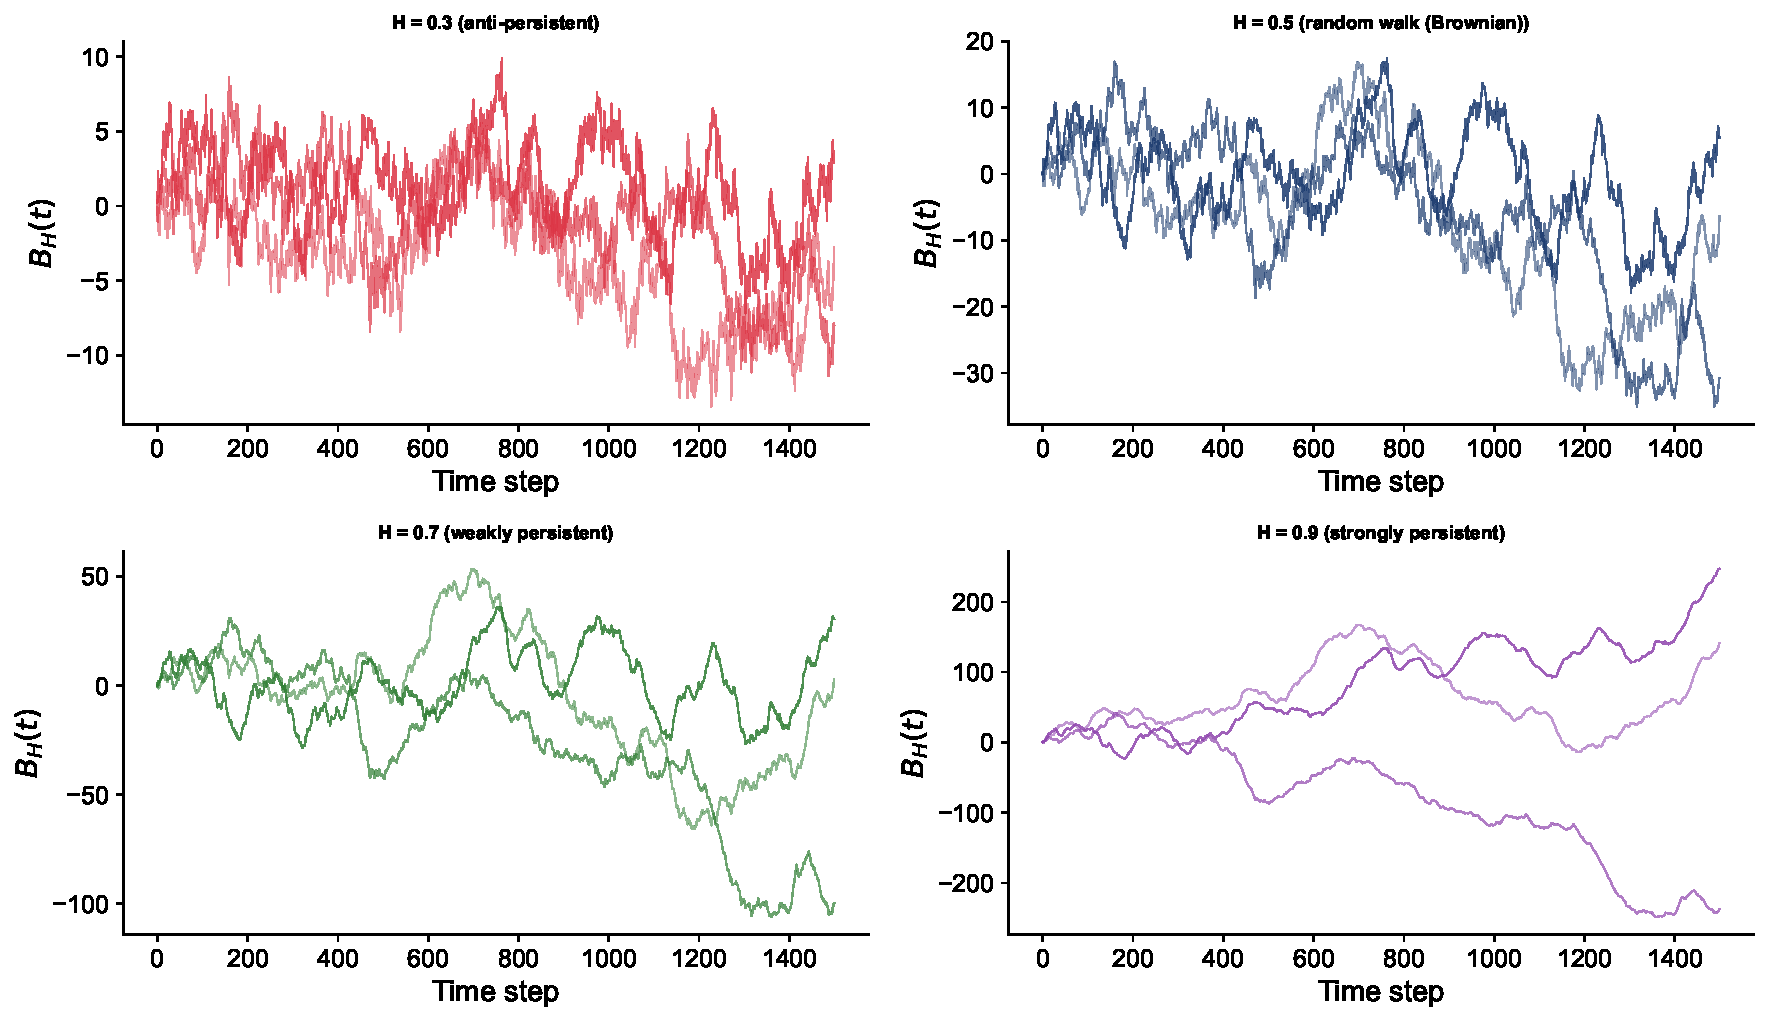
\includegraphics[height=4.0cm,keepaspectratio]{ch_fmh_fbm_paths.pdf}\\[1pt]
{\tiny\textcolor{MediumGray}{\textit{Traiectorii fBm: zimțate la $H=0{,}3$, netede la $H=0{,}9$.}}}
\figql{SFM\_ch\_fmh\_fractals: fbm\_paths}{https://github.com/QuantLet/Stat_fin_markets/tree/master/Quantlets/SFM_ch_fmh}
\end{column}
\end{columns}
\end{cminipage}
\end{frame}

% TASK 3: split slide ARFIMA în 2 frame-uri (overflow rezolvat)
\slidelevel{PhD}
\begin{frame}[shrink=15]{Procese ARFIMA: definiție (ARFIMA --- definition)}
\begin{cminipage}{0.95\textwidth}
\begin{alertblock}{Atenție: timp discret vs continuu}
\begin{itemize}\setlength{\itemsep}{0pt}
    \item \textbf{ARFIMA = timp discret}; \textbf{fBm = timp continuu}
    \item Legate prin $d = H - 1/2$ sub ipoteze de regularitate
\end{itemize}
\end{alertblock}

\begin{defn}[Proces ARFIMA]
$\{y_t\}$ urmează un model \textbf{ARFIMA}$(p, d, q)$ dacă:
\[
    \Phi(L)(1-L)^d y_t = \Theta(L)\varepsilon_t, \qquad \varepsilon_t \overset{\text{i.i.d.}}{\sim} (0, \sigma^2_\varepsilon)
\]
unde $d \in (-1/2, 1/2)$ este parametrul de \textbf{diferențiere fracționară}.
\end{defn}

\begin{itemize}\setlength{\itemsep}{0pt}
    \item Operatorul $(1-L)^d = \sum_{k=0}^{\infty} \binom{d}{k} (-L)^k = 1 - dL - \frac{d(1-d)}{2!}L^2 - \cdots$
    \item \textbf{Conexiunea cu Hurst}: pentru ARFIMA$(0, d, 0)$ avem $d = H - 1/2$
\end{itemize}
\end{cminipage}
\end{frame}

\slidelevel{PhD}
\begin{frame}[shrink=15]{Memorie lungă vs scurtă în timp discret (long vs short memory --- discrete time)}
\begin{cminipage}{0.95\textwidth}
\begin{block}{Memorie lungă ($0 < d < 1/2$, echivalent $H > 1/2$)}
\begin{itemize}\setlength{\itemsep}{0pt}
    \item Autocorelațiile descresc \textbf{hiperbolic}: $\rho(k) \sim C \, k^{2d-1}$
    \item Suma $\sum_{k=-\infty}^{\infty} |\rho(k)| = \infty$ (nesumabilă)
    \item Densitate spectrală $f(\lambda) \sim C_f |\lambda|^{-2d}$ când $\lambda \to 0$
\end{itemize}
\end{block}

\begin{block}{Memorie scurtă ($d = 0$, ARMA standard)}
\begin{itemize}\setlength{\itemsep}{0pt}
    \item Autocorelații cu decadere \textbf{exponențială}: $\rho(k) \sim \phi^k$
    \item $\sum |\rho(k)| < \infty$ (sumabilă)
\end{itemize}
\end{block}

\begin{exampleblock}{Antipersistent ($-1/2 < d < 0$, $H < 1/2$)}
\begin{itemize}\setlength{\itemsep}{0pt}
    \item Autocorelații negative pe termen lung; mean-reverting
\end{itemize}
\end{exampleblock}
\end{cminipage}
\end{frame}

\slidelevel{MSc}
\begin{frame}[shrink=15]{Densitatea spectrală a fGn (Spectral density of fGn)}
\begin{cminipage}{0.95\textwidth}
\begin{itemize}\setlength{\itemsep}{0pt}
    \item Densitatea spectrală de putere (power spectral density, PSD) a fGn:
    \[
        S(\omega) = 2 \sigma^2 \sin^2(\omega/2) \sum_{k=-\infty}^{\infty} \frac{1}{|2\pi k + \omega|^{2H+1}}
    \]
    \item \textbf{Aproximație la frecvențe joase} ($\omega \to 0$):
    \[
        S(\omega) \sim C_H |\omega|^{1 - 2H}
    \]
    \item \textbf{Trei regimuri spectrale}:
    \begin{itemize}\setlength{\itemsep}{0pt}
        \item $H < 0{,}5$: $S(\omega) \to 0$ când $\omega \to 0$ \,(\textit{,,blue noise''})
        \item $H = 0{,}5$: $S(\omega) =$ const \,(\textit{,,white noise''})
        \item $H > 0{,}5$: $S(\omega) \to \infty$ când $\omega \to 0$ \,(\textit{,,$1/f$-like'' / red noise})
    \end{itemize}
    \item \textbf{Estimator GPH} (Geweke \& Porter-Hudak, 1983): regresie log-periodogramă:
    \[
        \log I(\omega_j) = c - (2H - 1) \log \omega_j + \varepsilon_j
    \]
    pentru $\omega_j$ aproape de 0
    \item Implementat în \texttt{statsmodels.tsa.stattools.acf} și pachetul \texttt{arch}
\end{itemize}
\end{cminipage}
\end{frame}

\slidelevel{MSc}
\begin{frame}{Autocorelația fGn (fGn autocorrelation function)}
\begin{cminipage}{0.96\textwidth}
\centering
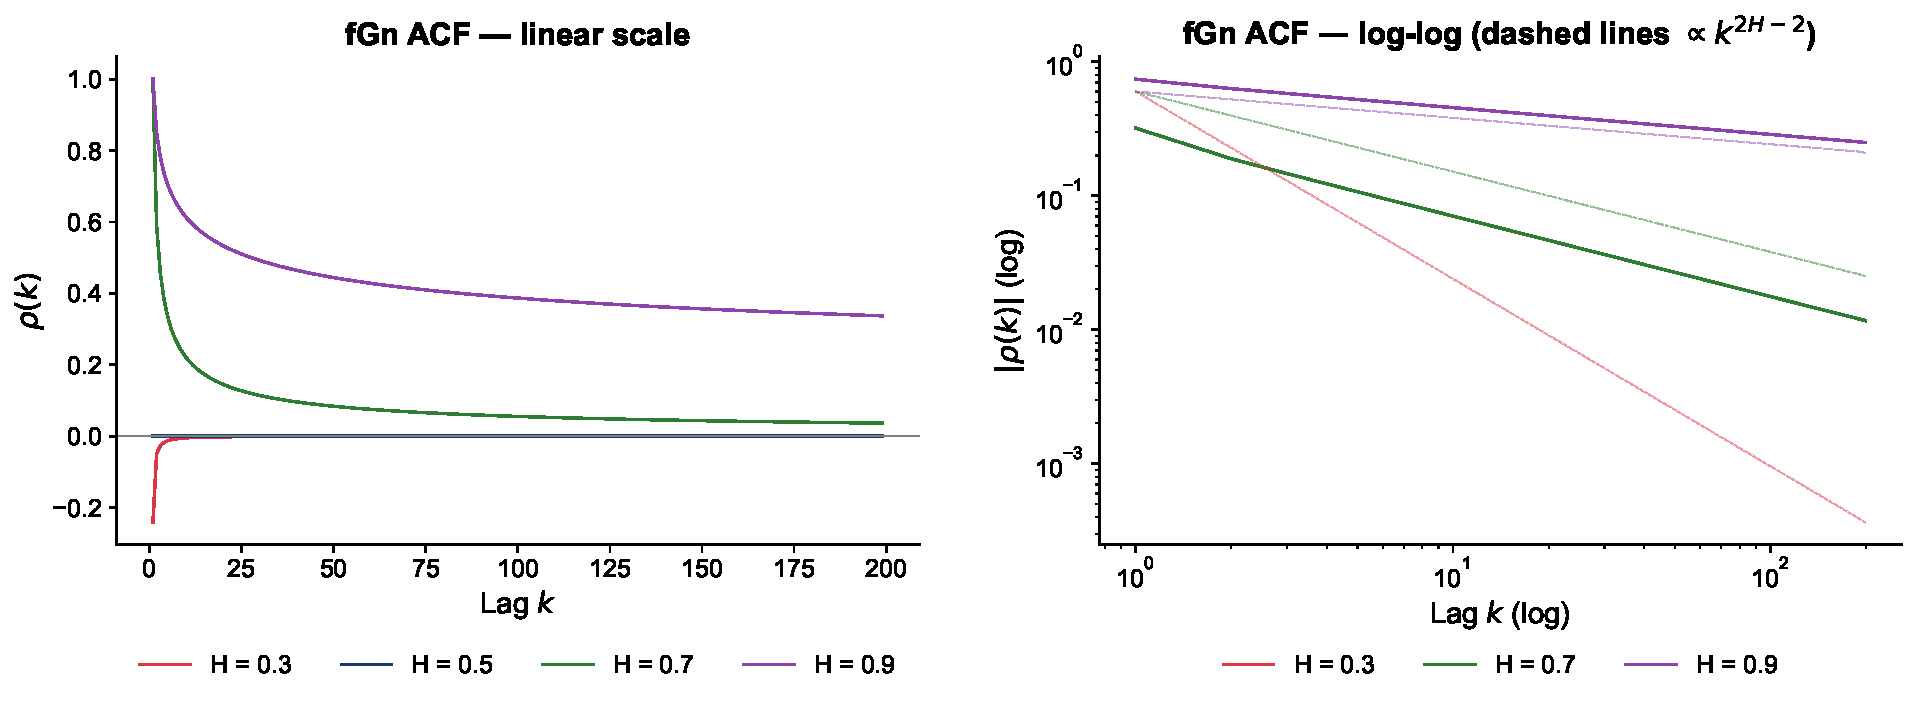
\includegraphics[height=5.0cm,keepaspectratio]{ch_fmh_fgn_acf.pdf}\\[2pt]
{\scriptsize\textcolor{MediumGray}{\textit{Stânga: ACF fGn în scală liniară pentru patru valori H. Dreapta: aceleași ACF în scală log-log; liniile întrerupte arată comportamentul $\sim k^{2H-2}$.}}}
\figql{SFM\_ch\_fmh\_extra: fgn\_acf}{https://github.com/QuantLet/Stat_fin_markets/tree/master/Quantlets/SFM_ch_fmh}
\end{cminipage}
\end{frame}

\slidelevel{Y3}
\begin{frame}[shrink=10]{Memorie lungă vs scurtă (long vs short memory)}
\begin{cminipage}{0.95\textwidth}
\centering
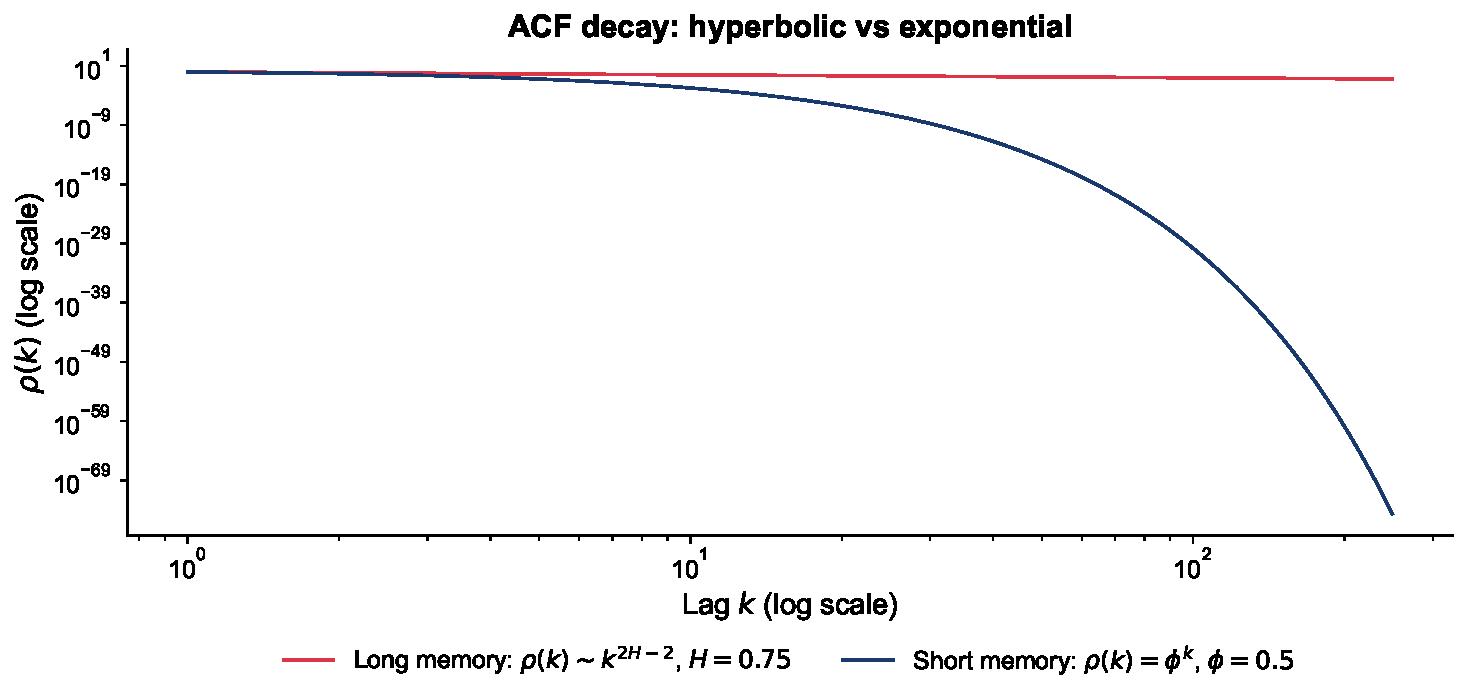
\includegraphics[height=5.0cm,keepaspectratio]{ch_fmh_lm_decay.pdf}\\[2pt]
{\scriptsize\textcolor{MediumGray}{\textit{Decadere autocorelație: ARFIMA/fBm (memorie lungă, hiperbolică) vs AR(1) (memorie scurtă, exponențială). Pe scală log-log, memoria lungă apare ca o dreaptă; cea scurtă curbează rapid.}}}
\figql{SFM\_ch\_fmh\_extra: lm\_decay}{https://github.com/QuantLet/Stat_fin_markets/tree/master/Quantlets/SFM_ch_fmh}
\end{cminipage}
\end{frame}

\slidelevel{PhD}
\begin{frame}[fragile, shrink=15]{Simularea fBm: metode (fBm simulation methods)}
\begin{cminipage}{0.95\textwidth}
\renewcommand{\arraystretch}{1.25}
\begin{center}
\small
\begin{tabular}{lll}
\toprule
\textbf{Metodă} & \textbf{Complexitate} & \textbf{Acuratețe} \\
\midrule
Cholesky & $O(n^2)$ memorie, $O(n^3)$ timp & Exactă \\
Hosking (1984) & $O(n^2)$ & Exactă, recursiv \\
Davies--Harte (1987) & $O(n \log n)$ & Exactă (matrice circulantă) \\
FFT-circular embedding & $O(n \log n)$ & Exactă pentru anumite acoperiri \\
Wavelet synthesis (Sellan) & $O(n)$ & Aproximativă \\
Random midpoint displacement & $O(n)$ & Aproximativă \\
Conditional simulation & $O(n^2)$ & Util pentru kriging \\
\bottomrule
\end{tabular}
\end{center}
\vspace{0.2cm}
\begin{itemize}\setlength{\itemsep}{0pt}
    \item \textbf{Recomandare}: \textbf{Davies--Harte} (circulant embedding) pentru $n$ mare
    \item Implementare Python: pachet \texttt{fbm} (Joachimiak, 2017):
\begin{lstlisting}
from fbm import FBM
f = FBM(n=10000, hurst=0.7, length=1, method='daviesharte')
fbm_path = f.fbm()         # fractional Brownian motion
fgn_path = f.fgn()         # fractional Gaussian noise (increments)
\end{lstlisting}
    \item \textbf{Atenție}: Davies-Harte cere ca matricea circulantă să fie pozitiv definită (eigenvalori $\geq 0$); pentru $H$ aproape de extreme, alegeți o acoperire mai mare
\end{itemize}
\end{cminipage}
\end{frame}

\slidelevel{MSc}
\begin{frame}{Scalarea varianței sub fBm (Variance scaling under fBm)}
\begin{cminipage}{0.96\textwidth}
\centering
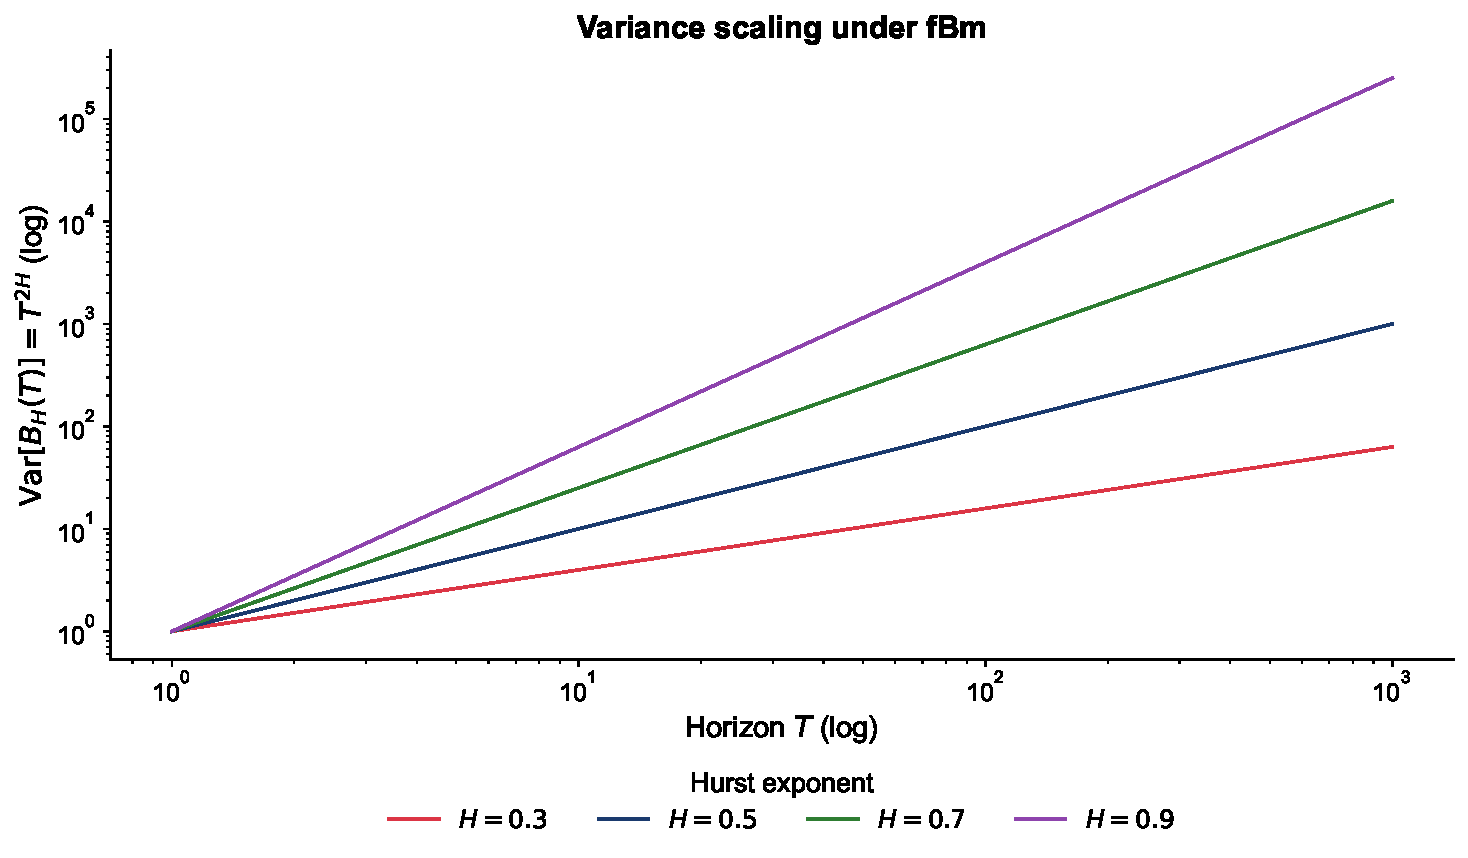
\includegraphics[height=5.4cm,keepaspectratio]{ch_fmh_var_scale_T2H.pdf}\\[2pt]
{\small\textcolor{MediumGray}{\textit{Scalarea $\Var[B_H(T)] = T^{2H}$ în log-log. Pantele drepte arată exponentul $2H$. Pentru $H=0,5$ avem scalarea Brownianului standard.}}}
\figql{SFM\_ch\_fmh\_extra: var\_scale}{https://github.com/QuantLet/Stat_fin_markets/tree/master/Quantlets/SFM_ch_fmh}
\end{cminipage}
\end{frame}

%#############################################################################
\section{Ipoteza Pieței Fractale (FMH)}
%#############################################################################

\slidelevel{Y3}
\begin{frame}[shrink=15]{EMH vs FMH: comparație directă}
\begin{cminipage}{0.95\textwidth}
\begin{columns}[T]
\begin{column}{0.48\textwidth}
\begin{block}{Ipoteza Pieței Eficiente (EMH)}
\begin{itemize}\setlength{\itemsep}{0pt}
    \item Toți investitorii au \textbf{același orizont} și reacționează identic
    \item Informația este reflectată \textbf{instantaneu} în prețuri
    \item Randamentele sunt \textbf{i.i.d.} cu varianță finită:
    $r_t \sim^{\text{i.i.d.}} F(\mu, \sigma^2)$
    \item Piețele sunt mereu în \textbf{echilibru}; arbitrajul dispare instant
    \item Prețurile urmează un \textbf{mers aleator} (Brown)
    \item Risc complet caracterizat de \textbf{varianță} $\sigma^2$
    \item \textbf{Hurst} $H = 0{,}5$
\end{itemize}
\end{block}
\end{column}
\begin{column}{0.48\textwidth}
\begin{alertblock}{Ipoteza Pieței Fractale (FMH)}
\begin{itemize}\setlength{\itemsep}{0pt}
    \item Investitorii operează pe \textbf{orizonturi multiple}: de la milisecunde la decenii
    \item Informația este \textbf{evaluată diferit} în funcție de orizont
    \item Stabilitatea piețelor depinde de \textbf{diversitatea} orizonturilor:
    Lichiditate $\propto$ Diversitate orizonturi
    \item Când orizonturile \textbf{colapsează} (panică) $\Rightarrow$ \textbf{lichiditatea dispare}, apar crah-uri
    \item Randamentele prezintă \textbf{autosimilaritate} și \textbf{memorie lungă}
    \item Risc caracterizat de \textbf{Hurst} $H$ \textbf{și} forma distribuțională
    \item De obicei $H \neq 0{,}5$ (cel mai des $H > 0{,}5$)
\end{itemize}
\end{alertblock}
\end{column}
\end{columns}
\end{cminipage}
\end{frame}

\slidelevel{Y3}
\begin{frame}[shrink=15]{Orizonturi multiple de investiție}
\begin{cminipage}{0.95\textwidth}
\begin{columns}[T]
\begin{column}{0.55\textwidth}
\begin{itemize}\setlength{\itemsep}{1pt}
    \item Ideea \textbf{centrală} a FMH: piețele sunt populate de investitori cu \textbf{orizonturi temporale foarte diferite}:
    \begin{itemize}\setlength{\itemsep}{0pt}
        \item \textbf{HFT (High-Frequency Traders)}: milisecunde--minute
        \item \textbf{Day traders}: ore--zile
        \item \textbf{Swing/position traders}: săptămâni--luni
        \item \textbf{Fonduri mutuale, hedge funds}: luni--ani
        \item \textbf{Fonduri de pensii, sovereign wealth}: ani--decenii
    \end{itemize}
    \item Fiecare clasă \textbf{evaluează informația diferit}:
    \begin{itemize}\setlength{\itemsep}{0pt}
        \item Un day trader reacționează puternic la un raport trimestrial
        \item Un fond de pensii ignoră zgomotul pe termen scurt
    \end{itemize}
    \item \textbf{Stabilitatea} cere diversitate de orizonturi: când traderii pe termen scurt vând, investitorii pe termen lung cumpără $\Rightarrow$ \textbf{lichiditate}
    \item Peters (1994): ,,Piața este ca un fractal --- elimină o scală și structura colapsează''
\end{itemize}
\end{column}
\begin{column}{0.42\textwidth}
\centering
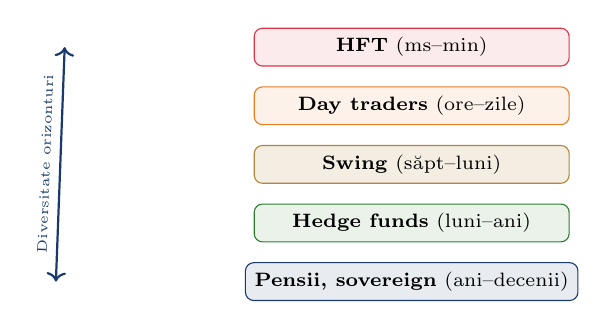
\begin{tikzpicture}[every node/.style={font=\scriptsize, align=left}, node distance=0.25cm]
\node[draw=Crimson, fill=Crimson!10, rounded corners=3pt, minimum width=4cm] (h1) {\textbf{HFT} (ms--min)};
\node[draw=Orange, fill=Orange!10, rounded corners=3pt, minimum width=4cm, below=of h1] (h2) {\textbf{Day traders} (ore--zile)};
\node[draw=Amber, fill=Amber!15, rounded corners=3pt, minimum width=4cm, below=of h2] (h3) {\textbf{Swing} (săpt--luni)};
\node[draw=Forest, fill=Forest!10, rounded corners=3pt, minimum width=4cm, below=of h3] (h4) {\textbf{Hedge funds} (luni--ani)};
\node[draw=MainBlue, fill=MainBlue!10, rounded corners=3pt, minimum width=4cm, below=of h4] (h5) {\textbf{Pensii, sovereign} (ani--decenii)};

\draw[<->, thick, MainBlue] ([xshift=-2.4cm]h1.west) -- ([xshift=-2.4cm]h5.west)
node[midway, sloped, above, font=\tiny] {Diversitate orizonturi};
\end{tikzpicture}

\vspace{0.4cm}

\begin{block}{Mecanismul stabilității}
\begin{itemize}\setlength{\itemsep}{0pt}
    \item \scriptsize Piață stabilă $\;\Longleftrightarrow\;$ distribuție largă de orizonturi
    \item \scriptsize Diversitate redusă $\;\Longrightarrow\;$ vulnerabilitate la șocuri
\end{itemize}
\end{block}
\end{column}
\end{columns}
\end{cminipage}
\end{frame}

\slidelevel{MSc}
\begin{frame}[shrink=15]{Crah-uri: când colapsează diversitatea orizonturilor}
\begin{cminipage}{0.95\textwidth}
\begin{itemize}\setlength{\itemsep}{0pt}
    \item Sub FMH, \textbf{lichiditatea} este consecința directă a diversității de orizonturi:
    \[
        \text{Lichiditate}_t \propto \sum_{h \in \mathcal{H}} w_h \cdot \text{Activitate}_{h,t}
    \]
    \item \textbf{Mecanismul crizei} (explicația FMH):
    \begin{enumerate}\setlength{\itemsep}{0pt}
        \item Un \textbf{șoc fundamental} (Lehman, COVID-19) afectează \textbf{toate orizonturile simultan}
        \item Investitorii pe termen lung \textbf{abandonează} strategiile lor obișnuite și adoptă comportament \textbf{pe termen scurt} (vânzare în panică)
        \item Distribuția orizonturilor \textbf{colapsează} $\Rightarrow$ toți investitorii au efectiv același orizont
        \item Fără diversitate, \textbf{lichiditatea evaporă}: nu există cumpărători pentru vânzători
        \item \textbf{Structura fractală} se rupe $\Rightarrow$ exponentul Hurst \textbf{se schimbă brusc}
    \end{enumerate}
    \item \textbf{Evidență empirică}:
    \begin{itemize}\setlength{\itemsep}{0pt}
        \item Criza 2008: $H_t$ pentru S\&P 500 a scăzut brusc spre $0{,}5$ (Dominique \& Rivera, 2011)
        \item COVID-19 (martie 2020): volatilitate fără precedent și iliquiditate pe măsură ce diversitatea orizonturilor a colapsat în câteva zile
    \end{itemize}
    \item FMH prezice că crah-urile nu sunt ,,lebede negre'' ci \textbf{eșecuri structurale} ale microstructurii pieței
\end{itemize}
\end{cminipage}
\end{frame}

% TASK 5: slide nou --- derivare formală horizon collapse
\slidelevel{MSc}
\begin{frame}[shrink=10]{Horizon collapse: derivare formală (formal derivation of horizon collapse)}
\begin{cminipage}{0.95\textwidth}
\begin{block}{Setup}
\begin{itemize}\setlength{\itemsep}{0pt}
    \item Investitori indexați după orizont $T_i \in \{1, 5, 22, 252\}$ zile (intraday, săptămânal, lunar, anual)
    \item Pondere cohortă $i$: $w_i$, cu $\sum w_i = 1$
    \item \textbf{Entropia distribuției orizonturilor}: $\mathcal{H}_{\text{horiz}} = -\sum_i w_i \log w_i$
\end{itemize}
\end{block}
\begin{alertblock}{Sub stres (criză)}
\begin{itemize}\setlength{\itemsep}{0pt}
    \item $w_i \to \delta_{i = \text{daytraders}}$ (toți colapsează la orizont scurt) $\Rightarrow$ $\mathcal{H}_{\text{horiz}} \to 0$
    \item \textbf{Implicație formală}: lichiditatea $L(t) \propto \mathcal{H}_{\text{horiz}} \Rightarrow L(t) \to 0$
\end{itemize}
\end{alertblock}
\begin{exampleblock}{Quantlet: simulare}
\begin{itemize}\setlength{\itemsep}{0pt}
    \item 4 cohorte, perturbare la $t = T/2$, plot $\mathcal{H}_{\text{horiz}}$ și $L(t)$ în timp
\end{itemize}
\end{exampleblock}
\quantlet{SFM\_ch10\_horizon\_collapse}{https://github.com/QuantLet/Stat_fin_markets/tree/master/Quantlets/SFM_ch10}
\end{cminipage}
\end{frame}

\slidelevel{Y3}
\begin{frame}[shrink=15]{Edgar Peters: pionier al FMH (Edgar E.~Peters)}
\begin{cminipage}{0.95\textwidth}
\begin{itemize}\setlength{\itemsep}{1pt}
    \item \textbf{Edgar E.~Peters} (1952--), economist și manager de fonduri american
    \item Director de cercetare la \textit{PanAgora Asset Management}
    \item \textbf{Două cărți fundamentale}:
    \begin{itemize}\setlength{\itemsep}{0pt}
        \item Peters (1991): \textit{Chaos and Order in the Capital Markets} --- prima formulare FMH în limba accesibilă practitioneri
        \item Peters (1994): \textit{Fractal Market Analysis} --- carte tehnică, R/S aplicat detaliat
    \end{itemize}
    \item \textbf{Contribuții cheie}:
    \begin{itemize}\setlength{\itemsep}{0pt}
        \item Aplicarea analizei R/S pe DJIA, S\&P 500 etc.
        \item Conceptul de \textbf{cycle length} (perioadă naturală a unei piețe) prin breakdown-ul scaling-ului R/S
        \item Linkul între \textbf{teoria haosului} (chaos theory) și piețe
        \item Ipoteza diversitatății orizonturilor de investiție
    \end{itemize}
    \item \textbf{Influențe}: Mandelbrot (1963, 1968), Lorenz (1963, atractor haotic), May (1976, hartă logistică)
    \item \textbf{Critica adresată Peters}: rezultatele R/S clasice sunt sensibile la lungimea seriei și autocorelații pe termen scurt (Lo, 1991) --- a fost ulterior validată empiric prin DFA și wavelet
\end{itemize}
\end{cminipage}
\end{frame}

\slidelevel{MSc}
\begin{frame}[shrink=15]{Modelul de procesare a informației (Information processing model)}
\begin{cminipage}{0.95\textwidth}
\begin{itemize}\setlength{\itemsep}{0pt}
    \item Sub FMH, fluxul informațional este mediat de \textbf{orizontul de investiție}:
    \[
        \text{Reacția}_h(t) = w_h \cdot I(t) \cdot \text{Discount}_h(\tau)
    \]
    unde $I(t)$ = șocul informațional, $\tau$ = orizontul de timp, $\text{Discount}_h$ = funcția de relevanță
    \item \textbf{Day trader}: răspunde puternic la informații pe orizont scurt; \textit{discount} rapid
    \item \textbf{Pension fund}: ignoră zgomotul, răspunde la fundamentale; \textit{discount} lent
    \item \textbf{Stabilitate}: dacă $w_h$ are o distribuție \textbf{largă} și \textbf{stabilă}, piața absoarbe șocurile
    \item \textbf{Instabilitate}: dacă toți investitorii adoptă același orizont, șocurile sunt amplificate
    \item Conexiune cu \textbf{teoria de difuziune anomală} (anomalous diffusion):
    \[
        \langle x^2(t) \rangle \sim t^{2H}, \quad H \neq 0{,}5
    \]
    indicând regim non-Brownian
\end{itemize}
\end{cminipage}
\end{frame}

\slidelevel{MSc}
\begin{frame}[shrink=15]{Microstructura pieței și FMH (Market microstructure)}
\begin{cminipage}{0.95\textwidth}
\begin{itemize}\setlength{\itemsep}{0pt}
    \item \textbf{Microstructura pieței} (market microstructure): cum se formează prețurile la nivel intraday/tick-level
    \item Componente ale FMH la nivel microstructural:
    \begin{itemize}\setlength{\itemsep}{0pt}
        \item \textbf{Market makers (HFT)}: orizont milisecunde, oferă lichiditate
        \item \textbf{Informed traders}: orizont minute--ore, exploatează informația
        \item \textbf{Liquidity traders}: orizont zile, motivați de necesități de cash
        \item \textbf{Long-term investors}: orizont luni--ani, valorizare fundamentală
    \end{itemize}
    \item \textbf{Bid-ask spread} ca indicator de stres: spread mic = diversitate de orizonturi, spread mare = colaps
    \item \textbf{Order flow imbalance}: măsură directă a colapsului orizonturilor
    \item \textbf{Mărimea ordinelor} (\textit{trade size distribution}) este \textbf{multifractală} (Plerou et al. 2002)
    \item \textbf{Fenomene la nivel microstructural}:
    \begin{itemize}\setlength{\itemsep}{0pt}
        \item Lead-lag effect (Epps, 1979): corelații cresc cu agregarea
        \item Volume--volatility relation (Karpoff, 1987)
        \item Realized volatility scaling (Andersen et al., 2003)
    \end{itemize}
\end{itemize}
\end{cminipage}
\end{frame}

\slidelevel{MSc}
\begin{frame}[shrink=15]{Bridging FMH cu finanțele comportamentale (Behavioral bridge)}
\begin{cminipage}{0.95\textwidth}
\begin{columns}[T]
\begin{column}{0.50\textwidth}
\begin{block}{De ce orizonturile colapsează?}
\begin{itemize}\setlength{\itemsep}{0pt}
    \item \textbf{Bias-uri comportamentale} (behavioral biases):
    \begin{itemize}\setlength{\itemsep}{0pt}
        \item \textbf{Loss aversion} (Kahneman--Tversky): pierderile dor de 2$\times$
        \item \textbf{Herding} (DeMarzo et al., 2003): copierea altor traderi
        \item \textbf{Disposition effect}: vânzarea câștigătorilor, păstrarea pierzătorilor
        \item \textbf{Recency bias}: ponderare excesivă a informației recente
    \end{itemize}
    \item Sub stres, biasele sincronizează orizonturile $\Rightarrow$ colaps fractal
\end{itemize}
\end{block}
\end{column}
\begin{column}{0.46\textwidth}
\begin{alertblock}{Adaptive Market Hypothesis (Lo, 2004)}
\begin{itemize}\setlength{\itemsep}{0pt}
    \item \textbf{Sinteză evoluționistă} a EMH, FMH și behavioral finance
    \item Eficiența \textbf{nu} e absolută, ci \textbf{depinde de competiția între strategii}
    \item ,,Survival of the fittest'' aplicat pieței
    \item Captură: $H_t$ variabil în timp
\end{itemize}
\end{alertblock}

\begin{block}{Sinteza FMH+AMH+Behavioral}
\begin{itemize}\setlength{\itemsep}{0pt}
    \item Piețele oscilează între \textbf{eficiență cvasi-completă} și \textbf{ineficiență}
    \item Eficiență $\Leftrightarrow$ orizonturi diverse
    \item Ineficiență $\Leftrightarrow$ panică, euforie, herding
    \item Toate observabile prin $H_t$ variabil în timp
\end{itemize}
\end{block}
\end{column}
\end{columns}
\end{cminipage}
\end{frame}

\slidelevel{Y3}
\begin{frame}[shrink=15]{Lichiditate și diversitate (Liquidity \& diversity)}
\begin{cminipage}{0.95\textwidth}
\begin{itemize}\setlength{\itemsep}{0pt}
    \item \textbf{Definiții ale lichidității} (liquidity):
    \begin{itemize}\setlength{\itemsep}{0pt}
        \item \textbf{Tightness}: bid-ask spread mic
        \item \textbf{Depth}: volum la fiecare nivel de preț
        \item \textbf{Resiliency}: viteza revenirii la echilibru după șoc
        \item \textbf{Immediacy}: viteza execuției unei tranzacții
    \end{itemize}
    \item Sub FMH: toate cele 4 dimensiuni depind de \textbf{diversitatea orizonturilor}
    \item \textbf{Indicatori empirici de stres}:
    \begin{itemize}\setlength{\itemsep}{0pt}
        \item Amihud illiquidity ratio: $|r_t| / V_t$ (Amihud, 2002)
        \item Kyle's lambda: $\lambda = $ price impact per unit volume (Kyle, 1985)
        \item VIX: volatilitate implicită (\textit{,,fear gauge''})
        \item TED spread (LIBOR -- T-Bills): risc credit interbancar
    \end{itemize}
    \item \textbf{Lecție FMH}: un \textbf{shock fundamental} (Lehman, COVID-19) poate accelera dispariția diversității de orizonturi $\Rightarrow$ \textbf{liquidity crisis}
    \item \textbf{Politici de stabilizare}: bănci centrale care intervin pe piețe de obligațiuni, ETF-uri = \textbf{,,artificial diversity providers''}
\end{itemize}
\end{cminipage}
\end{frame}

% TASK 5: slide nou --- critica long-memory
\slidelevel{MSc}
\begin{frame}[shrink=10]{Long-memory: regime shifts vs memorie reală (long memory --- spurious vs real)}
\begin{cminipage}{0.95\textwidth}
\begin{block}{Critica metodologică (literatură fundamentală)}
\begin{itemize}\setlength{\itemsep}{0pt}
    \item \textbf{Granger \& Ding (1996)}: nonliniaritatea poate genera \textit{spurious long memory}
    \item \textbf{Diebold \& Inoue (2001)}: $\hat{H}$ ridicat poate veni din regime shifts, nu din fBm real
    \item \textbf{Mikosch \& Stărică (2004)}: structural breaks $\Rightarrow$ spurious long memory
\end{itemize}
\end{block}

\begin{alertblock}{Implicație practică}
\begin{itemize}\setlength{\itemsep}{0pt}
    \item Înainte de a interpreta $\hat{H} > 0{,}5$ ca FMH, \textbf{testează stabilitatea}
\end{itemize}
\end{alertblock}

\begin{exampleblock}{Recomandare diagnostică}
\begin{itemize}\setlength{\itemsep}{0pt}
    \item (a) $\hat{H}$ pe sub-eșantioane (rolling window)
    \item (b) test de breakpoint à la Bai--Perron
    \item (c) DFA pe reziduuri post-detrending
\end{itemize}
\end{exampleblock}
\end{cminipage}
\end{frame}

% TASK 5: slide nou --- FMH vs AMH (Lo 2004) tabel comparativ
% TABLE-SLIDE
\slidelevel{MSc}
\begin{frame}{FMH vs AMH (Lo 2004) --- comparație formală (FMH vs AMH)}
\begin{cminipage}{0.96\textwidth}
\renewcommand{\arraystretch}{1.18}
\begin{center}
\scriptsize
\begin{tabular}{llll}
\toprule
\textbf{Aspect} & \textbf{EMH} & \textbf{FMH} & \textbf{AMH} \\
\midrule
Mecanism & Preferințe raționale & Orizonturi multiple & Competiție evolutivă \\
Eficiență & Mereu & Lichiditate ridicată & Context-dependent \\
Randamente & i.i.d. & Autosimilare $H \neq 0{,}5$ & Adaptive \\
Predictibilitate & Zero & Regimuri (mono/multi) & Variabilă în timp \\
Test primar & Variance ratio & Stabilitate $\hat{H}$ & Rolling Sharpe \\
\bottomrule
\end{tabular}
\end{center}

\begin{alertblock}{Notă critică}
\begin{itemize}\setlength{\itemsep}{0pt}
    \item FMH și AMH \textbf{nu sunt mutual exclusive} --- două lentile complementare
    \item Literatura recentă (Khuntia \& Pattanayak, 2018) tratează explicit hibridul
\end{itemize}
\end{alertblock}
\end{cminipage}
\end{frame}

% TASK 7: quiz formativ §9 FMH
\slidelevel{MSc}
\begin{frame}{Test rapid: §9 FMH (quiz FMH)}
\begin{cminipage}{0.95\textwidth}
\begin{enumerate}\setlength{\itemsep}{2pt}
    \item<1-> Ce înseamnă \textit{horizon collapse}?
    \begin{itemize}\setlength{\itemsep}{0pt}
        \item A) Toți investitorii dispar
        \item B) Distribuția orizonturilor colapsează la unul singur \onslide<2->{\textbf{← răspuns}}
        \item C) Volatilitatea crește
    \end{itemize}
    \item<3-> De ce duce horizon collapse la lichiditate scăzută?
    \begin{itemize}\setlength{\itemsep}{0pt}
        \item A) Dispare diversitatea preferințelor de tranzacționare \onslide<4->{\textbf{← răspuns}}
        \item B) Prețurile cresc
        \item C) Bid-ask spread scade
    \end{itemize}
    \item<5-> Diferența-cheie EMH vs FMH?
    \begin{itemize}\setlength{\itemsep}{0pt}
        \item A) FMH presupune mereu $H = 0{,}5$
        \item B) FMH admite orizonturi multiple și autosimilaritate \onslide<6->{\textbf{← răspuns}}
        \item C) EMH admite tail risk
    \end{itemize}
\end{enumerate}
\onslide<7->{\begin{block}{Sumar răspunsuri}1-B, 2-A, 3-B\end{block}}
\end{cminipage}
\end{frame}

%#############################################################################
\section{Multifractalitate}
%#############################################################################

\slidelevel{PhD}
\begin{frame}[shrink=20]{De la mono- la multifractalitate}
\begin{cminipage}{0.95\textwidth}
\begin{itemize}\setlength{\itemsep}{0pt}
    \item Un singur exponent Hurst $H$ (\textbf{monofractal}) poate fi insuficient: piețele reale prezintă \textbf{regimuri multiple} de scalare
    \item Mandelbrot, Fisher \& Calvet (1997): \textbf{Multifractal Model of Asset Returns} (MMAR)
    \item Log-prețul:
    \[
        \ln P(t) = B_H\bigl[\theta(t)\bigr]
    \]
    unde $B_H$ este fBm și $\theta(t)$ este o \textbf{,,trading time'' multifractală} (măsură aleatoare)
    \item Procesul este \textbf{multifractal} dacă momentele absolute scalează:
    \[
        \E\bigl[|X(t)|^q\bigr] = c(q) \cdot t^{\tau(q) + 1}
    \]
    cu $\tau(q)$ \textbf{neliniar} în $q$ (pentru monofractal: $\tau(q) = qH - 1$, liniar)
    \item \textbf{Spectrul multifractal} $f(\alpha)$: distribuția exponenților Hölder locali $\alpha$
    \[
        f(\alpha) = \inf_q \bigl\{q\alpha - \tau(q)\bigr\} \quad \text{(transformarea Legendre)}
    \]
    \item Spectru \textbf{larg} $\Rightarrow$ multifractalitate puternică (regiuni cu scalare locală foarte diferită)
    \item \textbf{Avantaje} față de modelele monofractale: capturează simultan \textbf{volatility clustering}, \textbf{cozi grele} și \textbf{intermittency}
\end{itemize}
\end{cminipage}
\end{frame}

\slidelevel{PhD}
\begin{frame}[shrink=15]{Exponentul Hölder local (local Hölder exponent)}
\begin{cminipage}{0.95\textwidth}
\begin{defn}[Hölder exponent local]
Funcția $f$ are exponent Hölder $\alpha$ în $t_0$ dacă există $C > 0$ și un polinom $P$ astfel încât:
\[
    |f(t) - P(t - t_0)| \leq C |t - t_0|^\alpha \quad \text{pentru } t \to t_0
\]
\textbf{Exponent Hölder maximal} (\textit{pointwise Hölder}):
\[
    \alpha(t_0) = \sup\bigl\{ \alpha : f \text{ are exponent Hölder } \alpha \text{ în } t_0 \bigr\}
\]
\end{defn}
\begin{itemize}\setlength{\itemsep}{0pt}
    \item Cuantifică \textbf{regularitatea locală} a funcției
    \item $\alpha(t_0) = 1 \Rightarrow$ funcția e diferențiabilă în $t_0$
    \item $\alpha(t_0) < 1 \Rightarrow$ singularitate locală
    \item Pentru fBm: $\alpha(t) = H$ aproape sigur, pentru orice $t$
    \item Pentru \textbf{multifractali}: $\alpha(t)$ variază cu $t$ $\Rightarrow$ \textbf{spectru de exponenți} $f(\alpha)$
\end{itemize}
\end{cminipage}
\end{frame}

\slidelevel{PhD}
\begin{frame}[shrink=15]{Cascade multiplicative (multiplicative cascades)}
\begin{cminipage}{0.95\textwidth}
\begin{columns}[T]
\begin{column}{0.40\textwidth}
\begin{itemize}\setlength{\itemsep}{0pt}
    \item Construite recursiv prin \textbf{redistribuire multiplicativă a masei}
    \item \textbf{Cascade binomială} (binomial cascade):
    \begin{itemize}\setlength{\itemsep}{0pt}
        \item Pas 0: masa $\mu_0 = 1$ pe $[0, 1]$
        \item Pas 1: $[0, 1/2]$ primește masa $p$, $[1/2, 1]$ primește $1-p$
        \item Pas $n$: redistribui în fiecare interval
    \end{itemize}
    \item Generalizări:
    \begin{itemize}\setlength{\itemsep}{0pt}
        \item Lognormal cascade
        \item Poisson multiplicative cascade
        \item Compound Poisson cascade (Calvet--Fisher)
    \end{itemize}
    \item \textbf{Aplicare în finanțe}: modelarea \textbf{volatility clustering} și volatility-volume correlation
\end{itemize}
\end{column}
\begin{column}{0.58\textwidth}
\centering
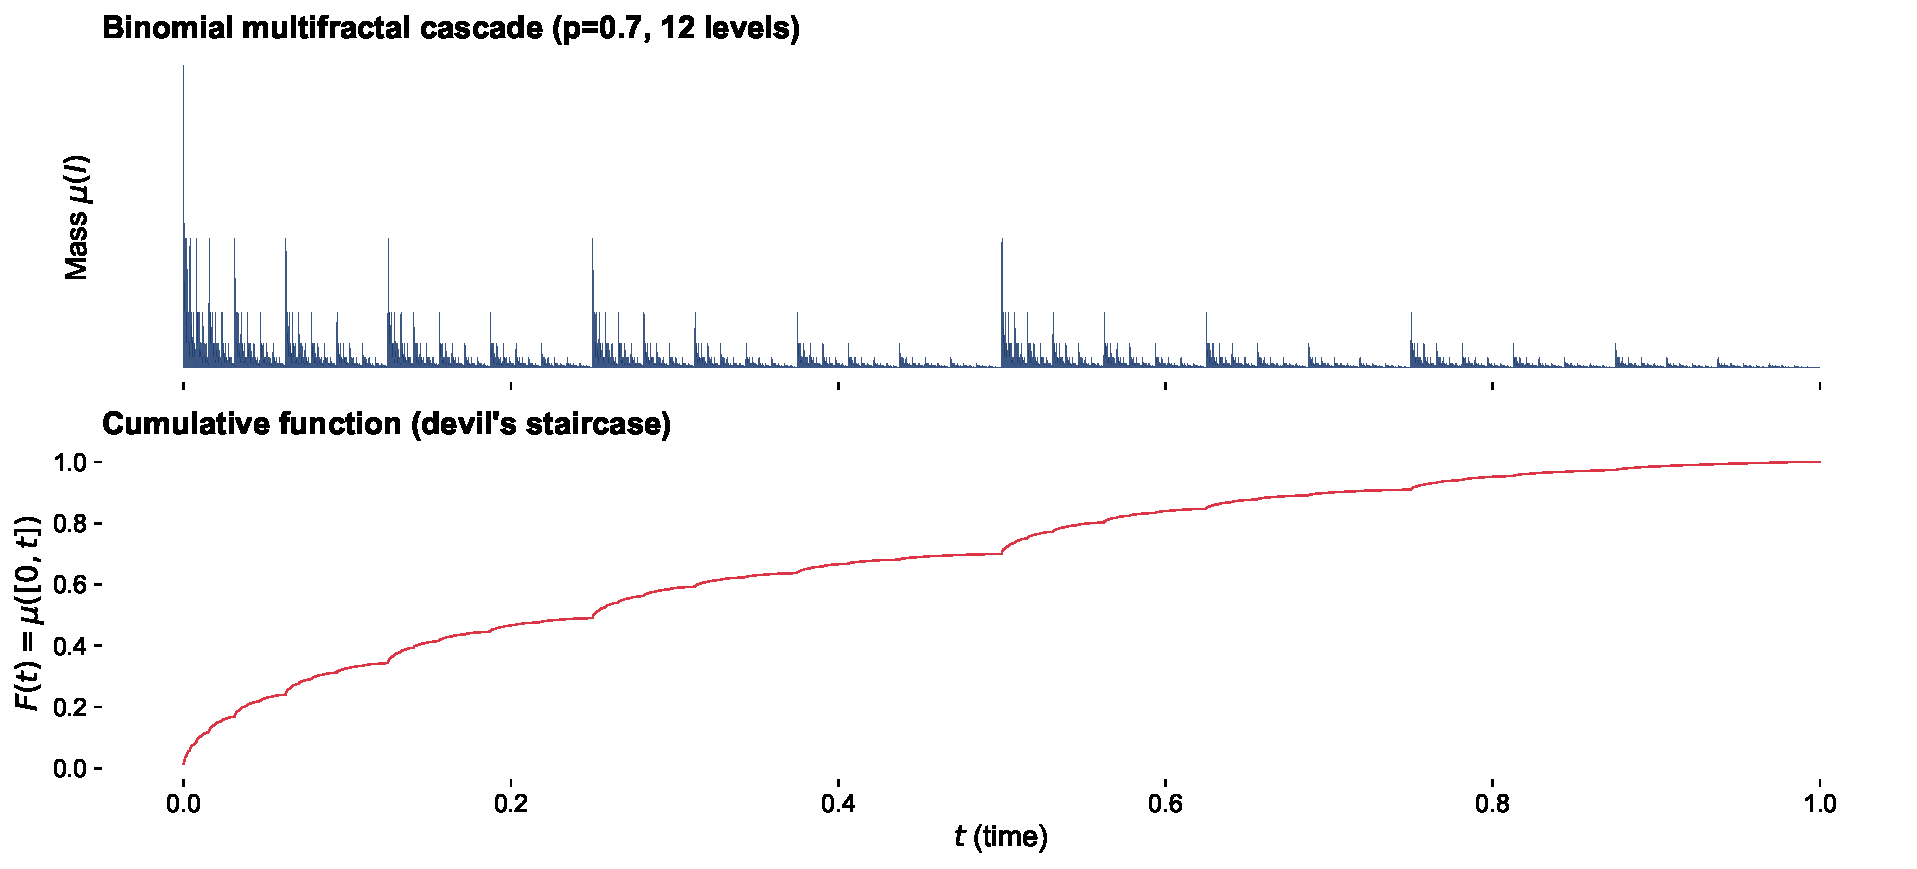
\includegraphics[width=\linewidth]{ch_fmh_multi_cascade.pdf}\\[2pt]
{\scriptsize\textcolor{MediumGray}{\textit{Sus: cascada binomială cu $p=0.7$ după 12 nivele. Jos: funcția cumulativă (,,devil's staircase'').}}}
\figql{SFM\_ch\_fmh\_extra: multi\_cascade}{https://github.com/QuantLet/Stat_fin_markets/tree/master/Quantlets/SFM_ch_fmh}
\end{column}
\end{columns}
\end{cminipage}
\end{frame}

\slidelevel{PhD}
\begin{frame}{Spectrul multifractal $f(\alpha)$ (multifractal spectrum)}
\begin{cminipage}{0.96\textwidth}
\centering
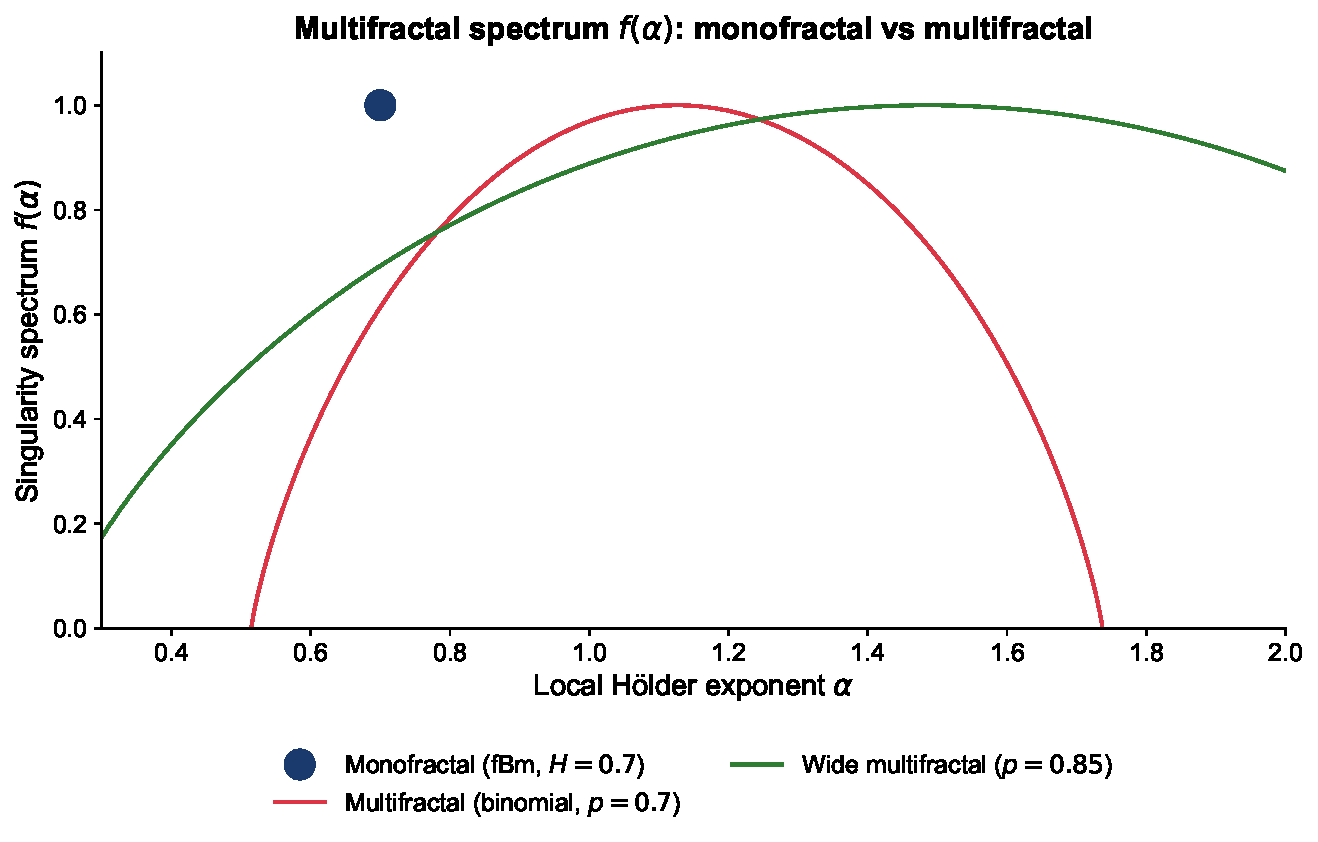
\includegraphics[height=5.0cm,keepaspectratio]{ch_fmh_spectrum.pdf}\\[2pt]
{\scriptsize\textcolor{MediumGray}{\textit{Spectrul multifractal: monofractalul are un singur punct $(\alpha=H, f(\alpha)=1)$. Multifractalul are un \textbf{interval} $[\alpha_{\min}, \alpha_{\max}]$ cu $f(\alpha) \leq 1$. Lățimea spectrului cuantifică ,,gradul de multifractalitate''.}}}
\figql{SFM\_ch\_fmh\_extra: spectrum}{https://github.com/QuantLet/Stat_fin_markets/tree/master/Quantlets/SFM_ch_fmh}
\end{cminipage}
\end{frame}

% TASK 3: split slide MMAR în 2 frame-uri (construcție / proprietăți+critică)
\slidelevel{PhD}
\begin{frame}[shrink=10]{MMAR --- construcția (Multifractal Model of Asset Returns)}
\begin{cminipage}{0.95\textwidth}
\begin{itemize}\setlength{\itemsep}{2pt}
    \item Mandelbrot, Fisher, Calvet (1997): \textbf{MMAR}
    \item \textbf{Pas 1}: trading time multifractal $\theta(t)$ (timp deformat)
    \[
        \theta(t) = \int_0^t \mu(ds), \quad \mu = \text{cascadă multiplicativă pozitivă}
    \]
    \item \textbf{Pas 2}: compunere cu fBm pentru log-preț
    \[
        \ln P(t) = B_H(\theta(t))
    \]
    \item Captură \textbf{simultană}: cozi grele, vol. clustering, long memory, multifractalitate
\end{itemize}
\end{cminipage}
\end{frame}

\slidelevel{PhD}
\begin{frame}[shrink=10]{MMAR --- proprietăți și critică (MMAR properties \& critique)}
\begin{cminipage}{0.95\textwidth}
\begin{block}{Proprietăți de scalare}
\begin{itemize}\setlength{\itemsep}{0pt}
    \item Scalarea momentelor: $\E[|\ln P(t+\tau) - \ln P(t)|^q] \sim \tau^{\tau_X(q)}$
    \item Compoziție: $\tau_X(q) = \tau_\theta(qH) - 1$
\end{itemize}
\end{block}
\begin{alertblock}{Critică și implementări}
\begin{itemize}\setlength{\itemsep}{0pt}
    \item \textbf{Estimare empirică}: foarte dificilă, mulți parametri
    \item \textbf{Critică}: nu e proces cu ,,real time'' bine-definit; greu de simulat exact
    \item \textbf{Implementări practice}: Calvet \& Fisher (2002), Lux (2008)
\end{itemize}
\end{alertblock}
\end{cminipage}
\end{frame}

\slidelevel{PhD}
\begin{frame}[shrink=15]{MSM: Markov-Switching Multifractal (Calvet \& Fisher 2004)}
\begin{cminipage}{0.95\textwidth}
\begin{itemize}\setlength{\itemsep}{0pt}
    \item \textbf{Markov-Switching Multifractal} (MSM): variantă \textbf{discretă} și \textbf{computațional tratabilă} a MMAR
    \item Volatility este produsul de $K$ multiplicatori independenți, fiecare cu propriul ,,clock'':
    \[
        \sigma_t^2 = \bar{\sigma}^2 \prod_{k=1}^K M_{k,t}
    \]
    \item Fiecare multiplicator $M_{k,t}$ urmează un \textbf{lanț Markov} cu 2 stări:
    \begin{itemize}\setlength{\itemsep}{0pt}
        \item Stare ,,High'': $m_0 \in (1, 2)$, probabilitate $1/2$
        \item Stare ,,Low'': $2 - m_0$, probabilitate $1/2$
    \end{itemize}
    \item \textbf{Frecvența switch-ului} pentru componenta $k$:
    \[
        \gamma_k = 1 - (1 - \gamma_K)^{(b^{k-K})}
    \]
    cu $\gamma_K \in (0,1)$ și $b > 1$
    \item Componenta 1 = orizont \textbf{lung} (rar switch); componenta $K$ = orizont \textbf{scurt} (switch des)
    \item \textbf{Avantaje MSM}: estimare prin \textbf{maximum likelihood} (recursivă), forecasting bun, captură multifractalitate
    \item Pachet R: \texttt{MSGARCH}, \texttt{rugarch}; Python: implementare proprie
\end{itemize}
\end{cminipage}
\end{frame}

\slidelevel{MSc}
\begin{frame}[shrink=15]{Aplicații MFDFA pe piețe reale (MFDFA real markets)}
\begin{cminipage}{0.95\textwidth}
\renewcommand{\arraystretch}{1.25}
\begin{center}
\small
\begin{tabular}{llll}
\toprule
\textbf{Piață} & \textbf{$h(2)$ (Hurst)} & \textbf{$\Delta\alpha = \alpha_{\max} - \alpha_{\min}$} & \textbf{Multifractal?} \\
\midrule
S\&P 500 (1990--2024) & $0{,}55$ & $0{,}45$ & Da, moderat \\
DAX 30 & $0{,}54$ & $0{,}42$ & Da, moderat \\
BET (BVB) & $0{,}65$ & $0{,}38$ & Da, slab \\
Bitcoin (2014--2024) & $0{,}53$ & $0{,}55$ & Da, puternic \\
EUR/USD (intraday) & $0{,}51$ & $0{,}30$ & Aproape monofractal \\
Aur (XAU) & $0{,}54$ & $0{,}40$ & Moderat \\
Brent oil & $0{,}53$ & $0{,}50$ & Puternic (turbulență $\sim$ piață) \\
\bottomrule
\end{tabular}
\end{center}
\vspace{0.2cm}
\begin{itemize}\setlength{\itemsep}{0pt}
    \item \textbf{Lățimea spectrului} $\Delta \alpha$ = măsură a multifractalității
    \item Forex e cel mai aproape de monofractal (lichiditate ridicată)
    \item Cripto și mărfuri au cele mai puternice multifractalități
    \item \textbf{Sursa multifractalității}: combinația \textbf{cozi grele} + \textbf{long memory} + \textbf{volatility clustering}
    \item \textbf{Studii Monte Carlo} (Kantelhardt et al. 2002): pot exista ,,multifractali aparenți'' din cauza dimensiunii finite
\end{itemize}
\end{cminipage}
\end{frame}

\slidelevel{PhD}
\begin{frame}[shrink=15]{Aplicare practică: forecasting volatilitate cu MFDFA}
\begin{cminipage}{0.95\textwidth}
\begin{itemize}\setlength{\itemsep}{0pt}
    \item \textbf{Idee}: folosiți spectrul multifractal $f(\alpha)$ ca features pentru ML/forecasting
    \item \textbf{Pipeline tipic}:
    \begin{enumerate}\setlength{\itemsep}{0pt}
        \item Calcul rolling MFDFA pe fereastră de 1 an
        \item Extragere features: $h(2)$, $\Delta\alpha$, asimetrie spectru, $\alpha_{\min}$, $\alpha_{\max}$
        \item Forecasting volatilitate / regim cu ML (e.g., LSTM, XGBoost)
    \end{enumerate}
    \item \textbf{Studii empirice}:
    \begin{itemize}\setlength{\itemsep}{0pt}
        \item Calvet \& Fisher (2008): MSM bate GARCH(1,1) pe forecasts pe orizont 10--30 zile
        \item Liu et al.\ (2020): MFDFA features cresc R$^2$ cu 5--10\% pe XGBoost
        \item Wei et al.\ (2018): predicție crizelor folosind $\Delta\alpha$ rolling
    \end{itemize}
    \item \textbf{Direcții moderne}:
    \begin{itemize}\setlength{\itemsep}{0pt}
        \item Combinare cu deep learning (Transformer, LSTM)
        \item Multifractal cross-correlation analysis (MFCCA)
        \item Wavelet leaders (Jaffard et al.) pentru estimare robustă
    \end{itemize}
    \item \textbf{Open source}: \href{https://github.com/LRydin/MFDFA}{MFDFA Python package}
\end{itemize}
\end{cminipage}
\end{frame}

%#############################################################################
\section{Evidență empirică}
%#############################################################################

\slidelevel{MSc}
\begin{frame}[shrink=20]{Estimări $\hat{H}$ pe clase de active}
\begin{cminipage}{0.95\textwidth}
\renewcommand{\arraystretch}{1.2}
\begin{center}
\begin{tabular}{llcc}
\toprule
\textbf{Clasă de active} & \textbf{Piață} & \textbf{$\hat{H}$ tipic} & \textbf{Metodă} \\
\midrule
Indici acțiuni & S\&P 500 & $0{,}55$--$0{,}62$ & R/S, DFA \\
Indici acțiuni & FTSE 100 & $0{,}53$--$0{,}60$ & DFA \\
Indici acțiuni & DAX & $0{,}54$--$0{,}61$ & R/S, DFA \\
Indici acțiuni & Nikkei 225 & $0{,}52$--$0{,}59$ & DFA \\
Piețe emergente & BIST 100 (Turcia) & $0{,}58$--$0{,}68$ & DFA \\
Piețe emergente & \textbf{BET (BVB)} & $0{,}60$--$0{,}72$ & R/S, DFA \\
Cripto & Bitcoin (BTC) & $0{,}50$--$0{,}75$ & DFA, wavelet \\
Cripto & Ethereum (ETH) & $0{,}52$--$0{,}70$ & DFA \\
Forex & EUR/USD & $0{,}50$--$0{,}55$ & R/S, DFA \\
Mărfuri & Aur (XAU) & $0{,}52$--$0{,}58$ & DFA \\
Obligațiuni & US 10Y Treasury & $0{,}55$--$0{,}65$ & R/S \\
\bottomrule
\end{tabular}
\end{center}
\vspace{0.2cm}
\begin{itemize}\setlength{\itemsep}{0pt}
    \item \textbf{Concluzii cheie}: majoritatea indicilor de acțiuni prezintă persistență ușoară ($H \approx 0{,}55$--$0{,}65$), consistentă cu FMH
    \item \textbf{Piețe emergente} (inclusiv BVB) au $H$ \textbf{mai mare} $\Rightarrow$ memorie lungă mai puternică, eficiență mai redusă
    \item \textbf{Cripto}: $H$ foarte variabil reflectă microstructură în evoluție și grade diferite de eficiență
    \item Forex are $H \approx 0{,}5$ (cel mai aproape de EMH) datorită \textbf{lichidității ridicate}
\end{itemize}
\end{cminipage}
\end{frame}

\slidelevel{MSc}
\begin{frame}[shrink=10]{Hurst rolling: $H_t$ ca semnal de criză}
\begin{cminipage}{0.96\textwidth}
\centering
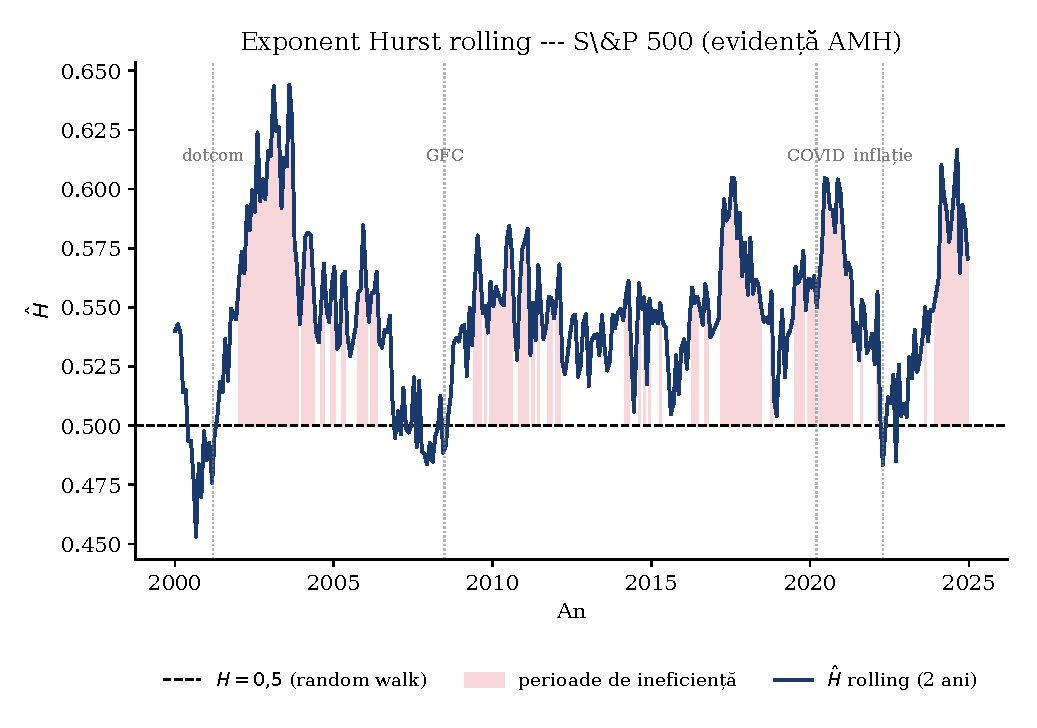
\includegraphics[height=5.0cm]{sfm_ch4_rolling_hurst.pdf}\\[2pt]
{\small\textcolor{MediumGray}{\textit{Exponentul Hurst rolling pe S\&P 500, fereastră 252 zile.}}}\\[6pt]
\begin{block}{Observații}
\begin{itemize}\setlength{\itemsep}{0pt}
    \item Variații sistematice ale lui $H_t$ în jurul valorii $0{,}5$
    \item Scăderi bruște spre $H = 0{,}5$ semnalează \textbf{colapsul orizonturilor} $\Rightarrow$ posibilă criză
    \item $H_t$ ridicat sugerează \textbf{trend dominant} și piață cu memorie
\end{itemize}
\end{block}
\end{cminipage}
\quantlet{SFM\_ch4\_rolling\_hurst}{https://github.com/QuantLet/Stat_fin_markets/tree/master/Quantlets/Ch_04/SFM_ch4_rolling_hurst}
\end{frame}

\slidelevel{MSc}
\begin{frame}{Evoluția eficienței pe clase de active (efficiency evolution)}
\begin{cminipage}{0.96\textwidth}
\centering
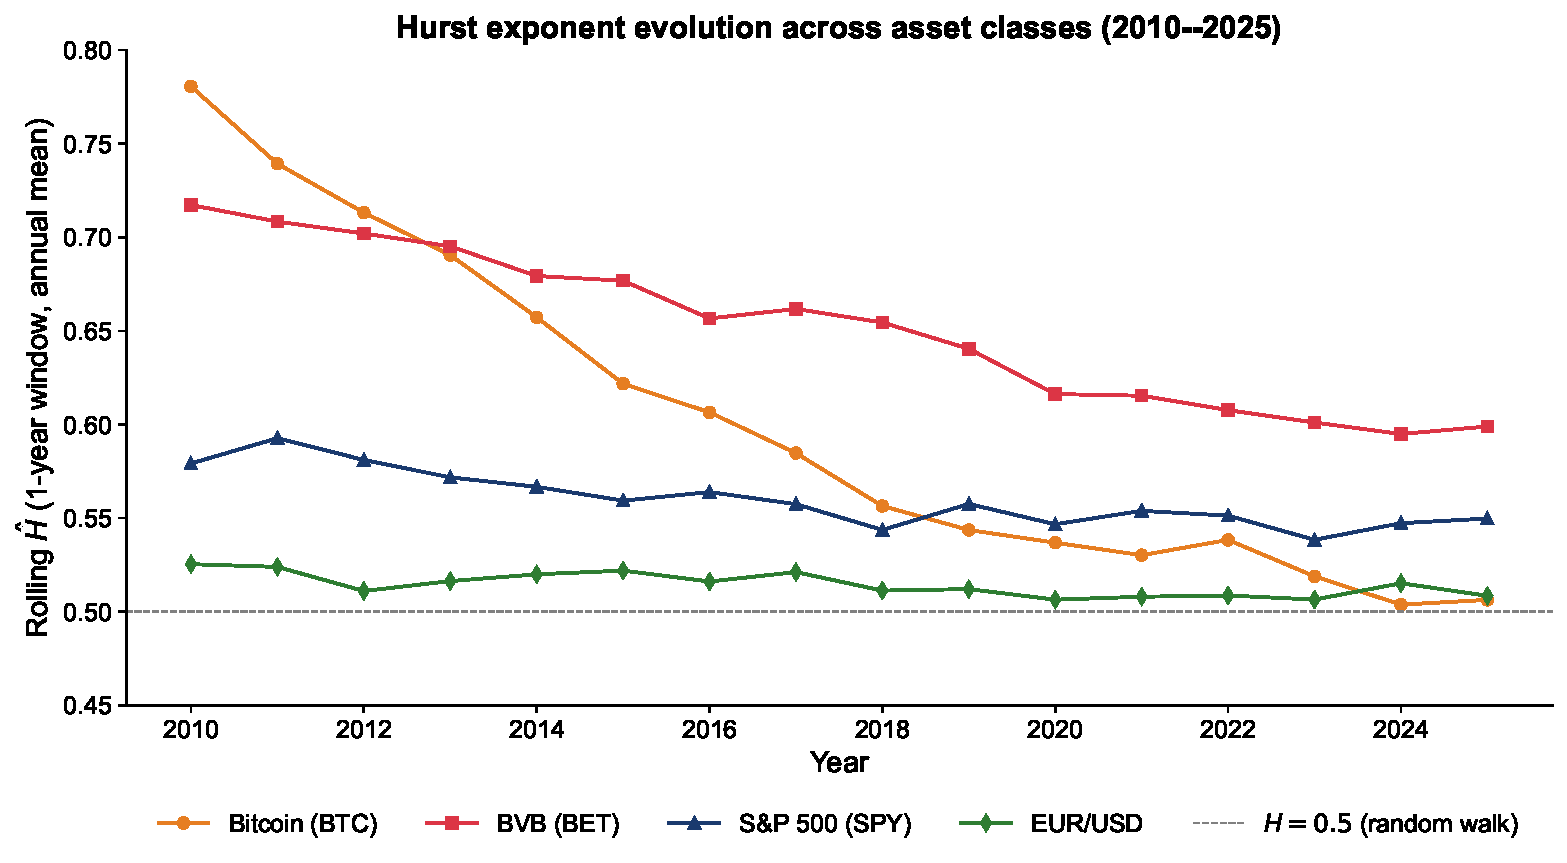
\includegraphics[height=5.4cm,keepaspectratio]{ch_fmh_eff_evolution.pdf}\\[2pt]
{\scriptsize\textcolor{MediumGray}{\textit{Exponentul Hurst rolling pentru BTC, BVB, S\&P 500, EUR/USD între 2010--2025. Tendința generală: convergență spre $H=0.5$ pe măsură ce piețele se maturizează.}}}
\figql{SFM\_ch\_fmh\_extra: eff\_evolution}{https://github.com/QuantLet/Stat_fin_markets/tree/master/Quantlets/SFM_ch_fmh}
\end{cminipage}
\end{frame}

\slidelevel{MSc}
\begin{frame}[shrink=15]{Comparație internațională (international comparison)}
\begin{cminipage}{0.95\textwidth}
\renewcommand{\arraystretch}{1.25}
\begin{center}
\small
\begin{tabular}{llll}
\toprule
\textbf{Țară} & \textbf{Indice} & \textbf{$\hat{H}$ tipic} & \textbf{Comentariu} \\
\midrule
SUA & S\&P 500 & $0{,}55$ & Cea mai eficientă piață mare \\
Marea Britanie & FTSE 100 & $0{,}55$ & Foarte lichidă \\
Germania & DAX & $0{,}57$ & Eficientă, structuri export \\
Franța & CAC 40 & $0{,}56$ & Lichidă, integrată EU \\
Japonia & Nikkei 225 & $0{,}55$ & Eficientă, dar cicluri lungi \\
China & SSE Composite & $0{,}65$ & Restricții capital, retail dominant \\
India & SENSEX & $0{,}63$ & Emergent maturizat \\
Brazilia & BOVESPA & $0{,}65$ & Volatilitate ridicată \\
Rusia & RTS & $0{,}68$ & Dependență commodities \\
Turcia & BIST 100 & $0{,}63$ & Inflație, volatilitate \\
\textbf{România} & \textbf{BET} & $\bm{0{,}65}$ & Lichiditate redusă, retail \\
Polonia & WIG20 & $0{,}60$ & Mai matură decât BVB \\
Ungaria & BUX & $0{,}62$ & Piață mică, dar matură \\
Cehia & PX & $0{,}60$ & Eficientă pentru dimensiune \\
\bottomrule
\end{tabular}
\end{center}
\vspace{0.2cm}
\begin{itemize}\setlength{\itemsep}{0pt}
    \item \textbf{Pattern general}: piețe \textbf{dezvoltate} au $H$ aproape de $0{,}5$; piețe \textbf{emergente} au $H \in [0{,}6, 0{,}7]$
    \item Determinanți: \textbf{lichiditate}, \textbf{participare instituțională}, \textbf{transparență}, \textbf{costuri tranzacționale}
\end{itemize}
\end{cminipage}
\end{frame}

\slidelevel{MSc}
\begin{frame}[shrink=15]{Hurst pe diferite frecvențe (Hurst at different frequencies)}
\begin{cminipage}{0.95\textwidth}
\renewcommand{\arraystretch}{1.25}
\begin{center}
\small
\begin{tabular}{lllll}
\toprule
\textbf{Frecvență (Frequency)} & \textbf{S\&P 500} & \textbf{BTC} & \textbf{EUR/USD} & \textbf{BET} \\
\midrule
1-min (intraday) & $0{,}48$--$0{,}52$ & $0{,}55$--$0{,}65$ & $0{,}50$--$0{,}53$ & N/A \\
5-min (intraday) & $0{,}50$--$0{,}55$ & $0{,}58$--$0{,}68$ & $0{,}51$--$0{,}54$ & N/A \\
1-oră & $0{,}52$--$0{,}57$ & $0{,}55$--$0{,}70$ & $0{,}52$--$0{,}55$ & N/A \\
Zilnic (daily) & $0{,}55$--$0{,}60$ & $0{,}55$--$0{,}70$ & $0{,}50$--$0{,}55$ & $0{,}60$--$0{,}65$ \\
Săptămânal (weekly) & $0{,}57$--$0{,}62$ & $0{,}50$--$0{,}65$ & $0{,}50$--$0{,}54$ & $0{,}62$--$0{,}68$ \\
Lunar (monthly) & $0{,}60$--$0{,}65$ & $0{,}55$--$0{,}70$ & $0{,}51$--$0{,}55$ & $0{,}65$--$0{,}72$ \\
\bottomrule
\end{tabular}
\end{center}
\vspace{0.2cm}
\begin{itemize}\setlength{\itemsep}{0pt}
    \item \textbf{Pattern frecvență}: $\hat{H}$ \textbf{crește} cu agregarea pentru majoritatea activelor
    \item \textbf{Excepții}: criptoactivele au comportament inversat la unele frecvențe
    \item \textbf{Implicare}: fractalitatea \textbf{nu este perfect auto-similară} la toate scalele $\Rightarrow$ \textbf{multifractalitate}
    \item \textbf{Cauze posibile}:
    \begin{itemize}\setlength{\itemsep}{0pt}
        \item Microstructure noise la frecvențe înalte (intraday)
        \item Cicluri economice la frecvențe joase (lunar)
        \item Activitate retail vs instituțional (diferite orizonturi)
    \end{itemize}
\end{itemize}
\end{cminipage}
\end{frame}

\slidelevel{PhD}
\begin{frame}[shrink=15]{Teste formale pentru $H = 0{,}5$ (formal tests)}
\begin{cminipage}{0.95\textwidth}
\renewcommand{\arraystretch}{1.25}
\begin{center}
\small
\begin{tabular}{lll}
\toprule
\textbf{Test} & \textbf{Statistică} & \textbf{Distribuție sub $H_0$} \\
\midrule
Lo (1991) modified R/S & $Q_n / \sqrt{n}$ & V (Lo, 1991, Tabel I) \\
Variance ratio (Lo--MacKinlay) & $M_2(q)$ & $\mathcal{N}(0,1)$ asimptotic \\
Multiple variance ratio & MV (Chow--Denning) & SMM (Hochberg) \\
GPH (Geweke--Porter-Hudak) & $\hat{d} - 0$ & $\mathcal{N}(0, \pi^2/24)$ \\
Robinson (1995) & $\hat{d}_R$ & $\mathcal{N}$ asimptotic \\
Whittle estimator & $\hat{H}_W$ & $\mathcal{N}$ asimptotic, eficient \\
Shimotsu \& Phillips (2005) ELW & $\hat{d}_{ELW}$ & $\mathcal{N}$, robust trenduri \\
\bottomrule
\end{tabular}
\end{center}
\vspace{0.2cm}
\begin{itemize}\setlength{\itemsep}{0pt}
    \item \textbf{Recomandare}: pentru aplicare profesională, raportați \textbf{minim 3 teste}
    \item \textbf{Combo standard}: Lo (1991) + Variance Ratio + GPH
    \item \textbf{Studii empirice cheie}:
    \begin{itemize}\setlength{\itemsep}{0pt}
        \item Lo (1991): respinge memoria lungă pe SP500 daily
        \item Greene \& Fielitz (1977): găsesc memorie lungă pe sub-perioade
        \item Caporale et al.\ (2018): cripto au $H$ semnificativ $> 0{,}5$
    \end{itemize}
    \item \textbf{Power problem}: testele au putere redusă pentru $H \approx 0{,}55$ și seri scurte
\end{itemize}
\end{cminipage}
\end{frame}

\slidelevel{MSc}
\begin{frame}[shrink=15]{Detectarea regimurilor folosind $\hat{H}_t$ (regime detection)}
\begin{cminipage}{0.95\textwidth}
\begin{itemize}\setlength{\itemsep}{0pt}
    \item Idee: monitorizarea \textbf{în timp real} a $\hat{H}_t$ ca \textbf{indicator de regim}
    \item Regimuri tipice:
    \begin{itemize}\setlength{\itemsep}{0pt}
        \item \textbf{Trending market}: $\hat{H}_t > 0{,}55$
        \item \textbf{Range-bound (lateral)}: $\hat{H}_t \approx 0{,}50$
        \item \textbf{Mean-reverting / panic}: $\hat{H}_t < 0{,}45$
    \end{itemize}
    \item \textbf{Threshold-uri pentru semnale}:
    \begin{itemize}\setlength{\itemsep}{0pt}
        \item $\hat{H}_t$ scade cu $> 2 \sigma$ în 5 zile $\Rightarrow$ \textbf{stress signal}
        \item $\hat{H}_t < 0{,}45$ pentru $> 10$ zile $\Rightarrow$ \textbf{panic signal}
        \item $\hat{H}_t$ stabil $> 0{,}60$ pentru $> 30$ zile $\Rightarrow$ \textbf{trend confirm}
    \end{itemize}
    \item \textbf{Strategii bazate pe Hurst regime}:
    \begin{itemize}\setlength{\itemsep}{0pt}
        \item Dacă $\hat{H}_t > 0{,}55$: \textbf{trend-following} (e.g., 200-day MA crossover)
        \item Dacă $\hat{H}_t < 0{,}45$: \textbf{mean-reversion} (e.g., RSI extreme)
        \item Dacă $\hat{H}_t \approx 0{,}5$: \textbf{neutral / stand aside}
    \end{itemize}
    \item \textbf{Pachet Python}: \texttt{hurst}, \texttt{nolds}, \texttt{MFDFA}
    \item \textbf{Aplicații algoritmice}: AHL/Man Group, Two Sigma, Renaissance folosesc semnale fractal-based
\end{itemize}
\end{cminipage}
\end{frame}

%#############################################################################
\section{Studii de caz}
%#############################################################################

\slidelevel{Y3}

% TASK 6: timeline introducere studii de caz
\slidelevel{Y3}
\begin{frame}[shrink=10]{Cronologia crizelor și evoluția FMH (timeline of crises)}
\begin{cminipage}{0.95\textwidth}
\begin{exampleblock}{De ce cronologic?}
\begin{itemize}\setlength{\itemsep}{0pt}
    \item Fiecare criză trasează o tipologie distinctă de \textbf{horizon collapse}
    \item Studiul în ordine cronologică expune \textbf{evoluția mecanismelor}
\end{itemize}
\end{exampleblock}

\vspace{0.2cm}
\centering
\begin{tabular}{ll}
\toprule
\textbf{An} & \textbf{Eveniment} \\
\midrule
1929 & Marea Depresiune (debutul crah-urilor moderne) \\
1987 & Black Monday (program trading) \\
1997--98 & Asia + LTCM (contagiune) \\
2008 & Global Financial Crisis \\
2010 & Flash Crash (HFT-driven) \\
2020 & COVID-19 (shock exogen) \\
2021--23 & GameStop, SVB (retail + duration risk) \\
\bottomrule
\end{tabular}
\end{cminipage}
\end{frame}

\slidelevel{Y3}
\begin{frame}[shrink=15]{Caz 1: Marea Depresiune 1929 (Great Depression)}
\begin{cminipage}{0.95\textwidth}
\begin{columns}[T]
\begin{column}{0.50\textwidth}
\begin{exampleblock}{Cronologie}
\begin{itemize}\setlength{\itemsep}{0pt}
    \item \textbf{Sept 1929}: DJIA atinge maximul (381)
    \item \textbf{24 oct 1929}: ,,Black Thursday'' --- $-9\%$ în prima oră
    \item \textbf{29 oct 1929}: ,,Black Tuesday'' --- $-12\%$ într-o zi
    \item \textbf{Iulie 1932}: DJIA atinge minimul (41), $-89\%$ față de vârf
    \item Recuperare la maximul anterior: 25 ani (nov 1954)
\end{itemize}
\end{exampleblock}

\begin{block}{Analiza retroactivă FMH}
\begin{itemize}\setlength{\itemsep}{0pt}
    \item Dificil de calculat $\hat{H}_t$ exact (date dinaintea computerelor)
    \item Mandelbrot \& Hudson (2004): estimează $\hat{H} \approx 0{,}65$ înainte de crah; \textbf{drop spre 0{,}45} în săptămâna critică
    \item Shiller (1981): excess volatility puzzle --- prețurile mai volatile decât fundamentele
\end{itemize}
\end{block}
\end{column}
\begin{column}{0.46\textwidth}
\begin{alertblock}{Importanța istorică}
\begin{itemize}\setlength{\itemsep}{0pt}
    \item Naștere SEC (1934), Glass-Steagall Act
    \item Învățare cheie: \textbf{margin trading} ($90\%$ leverage) a colapsat orizonturile peste noapte
    \item Sub FMH: amplificarea fractalității prin leverage = colaps liquidity catastrofal
\end{itemize}
\end{alertblock}

\begin{block}{Lecție pentru azi}
\begin{itemize}\setlength{\itemsep}{0pt}
    \item Reglementarea margin (Reg T, 50\%)
    \item Stress testing macroprudențial
    \item Monitorizare leverage sistemic (Basel III)
\end{itemize}
\end{block}
\end{column}
\end{columns}
\end{cminipage}
\end{frame}
\slidelevel{Y3}
\begin{frame}[shrink=15]{Caz 2: Black Monday 1987}
\begin{cminipage}{0.95\textwidth}
\begin{columns}[T]
\begin{column}{0.50\textwidth}
\begin{exampleblock}{Evenimente}
\begin{itemize}\setlength{\itemsep}{0pt}
    \item \textbf{19 oct 1987}: DJIA scade $-22{,}6\%$ într-o singură zi (cea mai mare scădere zilnică din istorie pentru SP500)
    \item Volume tranzacționate $4\times$ media
    \item Probabilitate sub gaussianitate: $\sim 10^{-50}$
    \item Fără ,,fundamental shock'' clar identificat
    \item Recuperare relativ rapidă: SP500 a închis anul 1987 pozitiv ($+2\%$)
\end{itemize}
\end{exampleblock}

\begin{block}{Cauze identificate}
\begin{itemize}\setlength{\itemsep}{0pt}
    \item \textbf{Portfolio insurance}: strategii dynamic hedging care vând automat pe cădere
    \item \textbf{Program trading}: amplificarea mișcărilor
    \item \textbf{Microstructure failure}: NYSE specialiști copleșiți
    \item Toate $\Rightarrow$ \textbf{colapsul orizonturilor} simultan
\end{itemize}
\end{block}
\end{column}
\begin{column}{0.46\textwidth}
\begin{alertblock}{Schimbări post-1987}
\begin{itemize}\setlength{\itemsep}{0pt}
    \item Introducerea \textbf{circuit breakers} (NYSE 1988):
    \begin{itemize}\setlength{\itemsep}{0pt}
        \item Halt trading la $-7\%$, $-13\%$, $-20\%$
    \end{itemize}
    \item Forțează \textbf{re-distribuirea orizonturilor} prin pauză
    \item Sub FMH: \textbf{circuit breakers = restaurarea diversității} prin întârziere temporală
    \item Eficacitate dezbătută (Subrahmanyam 1994 vs Goldstein \& Kavajecz 2000)
\end{itemize}
\end{alertblock}
\end{column}
\end{columns}
\end{cminipage}
\end{frame}
\slidelevel{MSc}
\begin{frame}[shrink=15]{Caz 3: Criza asiatică 1997 \& LTCM 1998}
\begin{cminipage}{0.95\textwidth}
\begin{columns}[T]
\begin{column}{0.50\textwidth}
\begin{exampleblock}{Criza Asiatică (1997)}
\begin{itemize}\setlength{\itemsep}{0pt}
    \item \textbf{2 iul 1997}: Thailanda devalorizează baht-ul
    \item Contagiune rapidă: Indonezia, Coreea, Filipine, Hong Kong
    \item Indici emergenți cad $-50\%$ în 6 luni
    \item IMF: bailout $\$120$B
    \item $\hat{H}$ pe piețe asiatice: drop de la $0{,}68$ la $0{,}50$ în 2 săpt
    \item \textbf{Lecție}: orizonturi colapsate în piețe corelate
\end{itemize}
\end{exampleblock}
\end{column}
\begin{column}{0.46\textwidth}
\begin{alertblock}{LTCM (1998)}
\begin{itemize}\setlength{\itemsep}{0pt}
    \item \textbf{Long-Term Capital Management}: hedge fund condus de laureați Nobel (Merton, Scholes)
    \item Folosea modele \textbf{gaussiene} pentru convergence trading
    \item Default rusesc (aug 1998): pierde $\$4{,}6$B în 4 luni
    \item Salvat de Fed-coordinated bailout
    \item \textbf{Cauza fundamentală}: presupunerea $H = 0{,}5$ a subestimat tail risk
    \item Sub FMH: corelațiile au crescut spre 1, lichiditatea a evaporat
    \item Mandelbrot a comentat public: ,,LTCM dovedește necesitatea modelelor fractale''
\end{itemize}
\end{alertblock}
\end{column}
\end{columns}
\end{cminipage}
\end{frame}

% TASK 6: GFC 2008 reconstruit (frame fusese pierdut accidental în reorder)
\slidelevel{MSc}
\begin{frame}[shrink=15]{Caz 4: Criza Financiară Globală 2008 (GFC)}
\begin{cminipage}{0.95\textwidth}
\begin{columns}[T]
\begin{column}{0.50\textwidth}
\begin{alertblock}{Cronologie}
\begin{itemize}\setlength{\itemsep}{0pt}
    \item \textbf{aug 2007}: BNP Paribas îngheață fonduri MBS
    \item \textbf{mar 2008}: căderea Bear Stearns
    \item \textbf{15 sep 2008}: faliment Lehman Brothers
    \item Indici globali pierd $-40\%$ în 6 luni; VIX urcă la $80$
    \item Bailout TARP $\$700$B (SUA), QE inițiat de Fed
\end{itemize}
\end{alertblock}
\end{column}
\begin{column}{0.46\textwidth}
\begin{block}{Citire FMH}
\begin{itemize}\setlength{\itemsep}{0pt}
    \item $\hat{H}$ pe S\&P 500: scade de la $\sim 0{,}55$ la $\sim 0{,}48$
    \item Long-only/value (orizont lung) pleacă $\Rightarrow$ rămân doar HFT
    \item \textbf{Horizon collapse} clasic: lichiditatea cade abrupt
    \item Tail risk subestimat de modele Gaussian/EMH: VaR violations $\gg$ așteptat
    \item \textbf{Lecție}: presupunerea iid $H = 0{,}5$ a sub-cuantificat severitatea
\end{itemize}
\end{block}
\end{column}
\end{columns}
\end{cminipage}
\end{frame}

\slidelevel{MSc}
\begin{frame}[shrink=15]{Caz 5: Flash Crash (6 mai 2010)}
\begin{cminipage}{0.95\textwidth}
\begin{columns}[T]
\begin{column}{0.50\textwidth}
\begin{exampleblock}{Cronologia evenimentului}
\begin{itemize}\setlength{\itemsep}{0pt}
    \item \textbf{14:32 ET}: Mutual fund Waddell \& Reed plasează ordin de $\$4{,}1$B în E-mini SP500 futures
    \item \textbf{14:42 ET}: SP500 cade $-9\%$ în 5 minute
    \item \textbf{14:45 ET}: HFTs retrag din ambele părți (sell + buy)
    \item \textbf{14:47 ET}: Liquiditate evaporă; spreaduri $> 10\%$ pe blue chips
    \item \textbf{14:52 ET}: Recuperare începe
    \item \textbf{15:08 ET}: SP500 înapoi la pre-crah
    \item Total: $\$1$ trilion volatilizat și recuperat în 36 minute
\end{itemize}
\end{exampleblock}
\end{column}
\begin{column}{0.46\textwidth}
\begin{alertblock}{Diagnostic FMH}
\begin{itemize}\setlength{\itemsep}{0pt}
    \item Toți participanții HFT au adoptat simultan \textbf{același orizont}: ,,nu mai oferi lichiditate''
    \item Diversitatea orizonturilor a colapsat în secunde
    \item $\hat{H}_t$ măsurat la frecvență second-by-second: drop de la $0{,}55$ la $0{,}30$ în 3 minute
    \item Anti-persistență temporară extremă
\end{itemize}
\end{alertblock}

\begin{block}{Reglementare post-2010}
\begin{itemize}\setlength{\itemsep}{0pt}
    \item Limit Up-Limit Down (LULD)
    \item Single-stock circuit breakers
    \item Consolidated audit trail (CAT)
\end{itemize}
\end{block}
\end{column}
\end{columns}
\end{cminipage}
\end{frame}
\slidelevel{Y3}
\begin{frame}[shrink=15]{Caz 6: COVID-19 (martie 2020)}
\begin{cminipage}{0.95\textwidth}
\begin{columns}[T]
\begin{column}{0.50\textwidth}
\begin{exampleblock}{Evenimente cheie}
\begin{itemize}\setlength{\itemsep}{0pt}
    \item \textbf{11 mar 2020}: OMS declară pandemie COVID-19
    \item \textbf{12 mar 2020}: SP500 scade $-9{,}5\%$ într-o singură zi (a doua cea mai mare după 1987)
    \item \textbf{16 mar 2020}: SP500 $-12\%$ (\textit{,,Black Monday II''})
    \item \textbf{23 mar 2020}: Fed lansează QE infinit; minim atins
    \item \textbf{Final aug 2020}: SP500 atinge nou maxim istoric
\end{itemize}
\end{exampleblock}

\begin{block}{Particularități fractale}
\begin{itemize}\setlength{\itemsep}{0pt}
    \item \textbf{Cel mai rapid bear market din istorie}: $-34\%$ în 33 de zile (vs 622 zile în 2008)
    \item Hurst rolling: a colapsat de la $\approx 0{,}58$ la $\approx 0{,}40$ în 2 săptămâni
    \item \textbf{Anti-persistență temporară}: $H < 0{,}5$ în plină criză (volatilitate alternantă, vânzare/cumpărare frenetică)
\end{itemize}
\end{block}
\end{column}
\begin{column}{0.46\textwidth}
\begin{alertblock}{Diferențe față de 2008}
\begin{itemize}\setlength{\itemsep}{0pt}
    \item \textbf{Șoc exogen} (sănătate publică), nu endogen (financiar)
    \item Răspuns fiscal-monetar \textbf{fără precedent}: $\$5T$ în 6 luni
    \item Recuperare în formă de \textbf{V} (vs forma de U în 2008)
    \item HFT și retail trading (Robinhood) au \textbf{amplificat} dinamica
    \item GameStop / meme stocks (ian 2021): eveniment fractal sui generis
\end{itemize}
\end{alertblock}

\vspace{0.15cm}

\begin{block}{Lecție}
\begin{itemize}\setlength{\itemsep}{0pt}
    \item $H_t$ rolling oferă \textbf{semnal precoce}
    \item Alarme la 1--2 zile înainte de minim
\end{itemize}
\end{block}
\end{column}
\end{columns}
\end{cminipage}
\end{frame}
\slidelevel{MSc}
\begin{frame}[shrink=15]{Caz 7: GameStop 2021 \& Silicon Valley Bank 2023}
\begin{cminipage}{0.95\textwidth}
\begin{columns}[T]
\begin{column}{0.50\textwidth}
\begin{exampleblock}{GameStop short squeeze (ian 2021)}
\begin{itemize}\setlength{\itemsep}{0pt}
    \item Retail traders pe r/wallstreetbets coordoneză cumpărări
    \item GME: $+1500\%$ în 2 săptămâni
    \item Hedge funds short forced cover (Melvin Capital pierde $\$6$B)
    \item Robinhood blochează cumpărări (28 ian 2021)
    \item $\hat{H}$ rolling pe GME: explodează la $0{,}85$ (super-trend) apoi cade la $0{,}30$ (panic)
    \item \textbf{Sub FMH}: o nouă clasă de retail traders (homogeneous horizon!) = colaps fractal nou
\end{itemize}
\end{exampleblock}
\end{column}
\begin{column}{0.46\textwidth}
\begin{alertblock}{Silicon Valley Bank (mar 2023)}
\begin{itemize}\setlength{\itemsep}{0pt}
    \item \textbf{8 mar 2023}: SVB anunță $\$1{,}8$B pierderi pe Treasuries
    \item \textbf{9 mar 2023}: Bank run \textbf{digital} prin Slack/Twitter; $\$42$B retrași într-o zi
    \item \textbf{10 mar 2023}: FDIC închide SVB (cel mai mare faliment bancar US din 2008)
    \item Contagiune: Signature Bank, First Republic Bank
    \item \textbf{Particularitate}: \textbf{social media} amplifică viteza colapsului orizonturilor
    \item Bank run-ul tradițional dura zile; cel digital a durat \textbf{ore}
\end{itemize}
\end{alertblock}

\begin{block}{Lecție FMH 2023}
\begin{itemize}\setlength{\itemsep}{0pt}
    \item \textbf{Tehnologia} accelerează colapsul orizonturilor
    \item Reglementarea trebuie să prevadă \textbf{ritmul digital}
\end{itemize}
\end{block}
\end{column}
\end{columns}
\end{cminipage}
\end{frame}
\slidelevel{MSc}
\begin{frame}[shrink=15]{Deep-dive A: Bursa de Valori București (BVB)}
\begin{cminipage}{0.95\textwidth}
\begin{columns}[T]
\begin{column}{0.50\textwidth}
\begin{itemize}\setlength{\itemsep}{0pt}
    \item \textbf{BET} este indicele principal (top 21 emitenți, free-float adjusted)
    \item Studii (Tilfani \& El Boukfaoui, 2020; Pele \& Mazurencu-Marinescu, 2014): $\hat{H}_{\text{BET}} \in [0{,}60, 0{,}72]$
    \item \textbf{Mai mare} decât piețele dezvoltate $\Rightarrow$ \textbf{eficiență redusă, memorie lungă}
    \item Posibile cauze:
    \begin{itemize}\setlength{\itemsep}{0pt}
        \item Lichiditate redusă (volume mici)
        \item Concentrare pe câțiva emitenți (FP, BRD, TLV, SNG)
        \item Investitori retail dominanți pe orizonturi similare
        \item Acoperire analitică limitată
    \end{itemize}
    \item \textbf{Implicații practice:}
    \begin{itemize}\setlength{\itemsep}{0pt}
        \item Strategii de \textit{momentum} pot funcționa mai bine decât pe SPY
        \item VaR clasic subestimează riscul cu $\sim 30\%$
        \item Diversificare internațională esențială
    \end{itemize}
\end{itemize}
\end{column}
\begin{column}{0.46\textwidth}
\begin{block}{Promovare BVB la \textit{Emerging Market}}
\begin{itemize}\setlength{\itemsep}{0pt}
    \item Sept 2020: FTSE Russell promovează BVB
    \item Studiu pre/post: $\hat{H}$ a scăzut de la $0{,}68$ la $0{,}62$ (mai eficientă)
    \item Volume crescute, mai mulți investitori străini $\Rightarrow$ \textbf{diversitate de orizonturi crescută}
    \item Lichiditate îmbunătățită $\Rightarrow$ defractalizare parțială
\end{itemize}
\end{block}

\vspace{0.2cm}

\begin{exampleblock}{Concluzie FMH pentru BVB}
\begin{itemize}\setlength{\itemsep}{0pt}
    \item Pe măsură ce piața devine mai \textbf{matură} și \textbf{lichidă}, $\hat{H} \to 0{,}5$
    \item Confirmă teoria FMH: diversitatea orizonturilor crește $\Rightarrow$ eficiență
\end{itemize}
\end{exampleblock}
\end{column}
\end{columns}
\end{cminipage}
\end{frame}
\slidelevel{MSc}
\begin{frame}[shrink=15]{Deep-dive B: Bitcoin --- evoluția eficienței}
\begin{cminipage}{0.95\textwidth}
\begin{columns}[T]
\begin{column}{0.55\textwidth}
\begin{itemize}\setlength{\itemsep}{0pt}
    \item \textbf{2010--2014} (faza ,,nascentă''): $\hat{H}_{\text{BTC}} \approx 0{,}70$--$0{,}80$
    \begin{itemize}\setlength{\itemsep}{0pt}
        \item Memorie lungă puternică
        \item Trenduri multilunare clare
        \item Piață foarte ineficientă
    \end{itemize}
    \item \textbf{2015--2018} (,,maturizare''): $\hat{H}_{\text{BTC}} \approx 0{,}55$--$0{,}65$
    \begin{itemize}\setlength{\itemsep}{0pt}
        \item Apariția futures-urilor BTC pe CME (dec 2017)
        \item Investitori instituționali încep să intre
    \end{itemize}
    \item \textbf{2019--prezent}: $\hat{H}_{\text{BTC}} \approx 0{,}50$--$0{,}55$
    \begin{itemize}\setlength{\itemsep}{0pt}
        \item Aproape de mers aleator
        \item ETF-uri spot BTC aprobate (ian 2024)
        \item Piață semi-eficientă
    \end{itemize}
    \item \textbf{Concluzie:} BTC ilustrează \textbf{tranziția} de la o piață fractală pură (puține orizonturi, ineficient) la o piață cvasi-eficientă (multe orizonturi, FX-like)
\end{itemize}
\end{column}
\begin{column}{0.40\textwidth}
\begin{alertblock}{Observații cheie}
\begin{itemize}\setlength{\itemsep}{0pt}
    \item \textbf{Halving-urile} (la fiecare 4 ani) introduc \textbf{ciclu fractal} suplimentar
    \item Multifractalitate semnificativă: spectrul $f(\alpha)$ este \textbf{larg}
    \item Evenimente cu impact: Mt.Gox 2014, China ban 2017, Terra 2022, FTX 2022
    \item Fiecare ,,colaps'' a reset-at temporar $\hat{H}$ în sus (memorie lungă revenită)
\end{itemize}
\end{alertblock}

\vspace{0.2cm}

{\scriptsize \textbf{Quantlet related:} \texttt{SFM\_ch4\_crypto\_eff} (Cap. 4)}
\end{column}
\end{columns}
\end{cminipage}
\end{frame}

% TASK 7: quiz formativ §12 Studii de caz
\slidelevel{Y3}
\begin{frame}{Test rapid: §12 Studii de caz (quiz crisis pattern)}
\begin{cminipage}{0.95\textwidth}
\begin{enumerate}\setlength{\itemsep}{2pt}
    \item<1-> Profil ,,$\hat{H}$ scade brusc + volatilitate ridicată + lichiditate evaporată'' este caracteristic la:
    \begin{itemize}\setlength{\itemsep}{0pt}
        \item A) Toate crizele majore (1929, 1987, 2008, 2020) \onslide<2->{\textbf{← răspuns}}
        \item B) Doar crize valutare
        \item C) Doar crize HFT-driven
    \end{itemize}
    \item<3-> Flash Crash 2010 a fost cauzat în principal de:
    \begin{itemize}\setlength{\itemsep}{0pt}
        \item A) Politică monetară
        \item B) Algoritmi HFT și fragmentarea pieței \onslide<4->{\textbf{← răspuns}}
        \item C) Inflație
    \end{itemize}
    \item<5-> LTCM 1998 ilustrează:
    \begin{itemize}\setlength{\itemsep}{0pt}
        \item A) Eficiența perfectă a pieței
        \item B) Eșecul modelelor Gaussian la tail risk \onslide<6->{\textbf{← răspuns}}
        \item C) Importanța orizontului scurt
    \end{itemize}
\end{enumerate}
\onslide<7->{\begin{block}{Sumar răspunsuri}1-A, 2-B, 3-B\end{block}}
\end{cminipage}
\end{frame}

\section{Implicații pentru managementul riscului}
%#############################################################################

\slidelevel{MSc}
\begin{frame}[shrink=15]{De ce contează FMH pentru risk management}
\begin{cminipage}{0.95\textwidth}
\begin{itemize}\setlength{\itemsep}{0pt}
    \item \textbf{Scalarea volatilității} (Basel III, FRTB):
    \begin{itemize}\setlength{\itemsep}{0pt}
        \item Regula clasică ,,$\sqrt{T}$'' presupune $H = 0{,}5$
        \item Sub FMH: $\sigma_{\text{T-day}} = \sigma_{\text{1-day}} \cdot T^{H}$
        \item Pentru $H = 0{,}6$, $T = 250$ (1 an): $\sigma_{\text{anual}} = \sigma_{\text{zilnic}} \cdot 250^{0{,}6} \approx 27{,}5 \cdot \sigma_{\text{zilnic}}$
        \item În loc de $\sqrt{250} \approx 15{,}8 \cdot \sigma_{\text{zilnic}}$ $\Rightarrow$ \textbf{eroare de aproape $74\%$}
    \end{itemize}
    \item \textbf{Value-at-Risk} (VaR):
    \begin{itemize}\setlength{\itemsep}{0pt}
        \item VaR clasic gaussian subestimează cozile (vezi Cap. 2--3)
        \item VaR sub fBm: $\text{VaR}_\alpha(T) = \mu T - \sigma T^H z_\alpha$
        \item Diferență de $20\text{--}40\%$ pe orizonturi de 1 an
    \end{itemize}
    \item \textbf{Detectare de regim} (early warning):
    \begin{itemize}\setlength{\itemsep}{0pt}
        \item Monitorizare $\hat{H}_t$ rolling
        \item Scădere bruscă $\hat{H}_t \to 0{,}5$ (sau sub) $\Rightarrow$ \textit{,,collapse of horizons''}
        \item Trigger pentru reducerea expunerii / hedging
    \end{itemize}
    \item \textbf{Allocation portofoliu}:
    \begin{itemize}\setlength{\itemsep}{0pt}
        \item Active cu $H$ mare: tendință puternică $\Rightarrow$ favorizează strategii \textbf{trend-following}
        \item Active cu $H$ mic: mean-reverting $\Rightarrow$ favorizează strategii \textbf{contrarian/value}
    \end{itemize}
    \item \textbf{Multifractal stress testing}: scenarii cu spectru larg $f(\alpha)$
\end{itemize}
\end{cminipage}
\end{frame}

\slidelevel{PhD}
\begin{frame}[shrink=20]{FMH și agenda contemporană de cercetare}
\begin{cminipage}{0.95\textwidth}
\begin{itemize}\setlength{\itemsep}{0pt}
    \item \textbf{Adaptive Market Hypothesis} (Lo, 2004; vezi Cap. 4): sinteză evoluționistă a EMH și FMH; eficiența \textbf{variază în timp}
    \item \textbf{High-frequency fractality}: $H$ pe scale de ms--secunde; evidență pentru ,,fractal microstructure'' (Bouchaud et al., 2018)
    \item \textbf{Multifractal portfolio theory}: extinderea Markowitz pentru spectre $f(\alpha)$ neechilibrate
    \item \textbf{Rough volatility} (Gatheral, Jaisson, Rosenbaum, 2018): volatilitatea log-vol-ului are $H \approx 0{,}1$ (foarte rough!)
    \item \textbf{Machine learning}: estimatori neuronali pentru $H$ și $f(\alpha)$; învățare auto-supervizată pe traiectorii
    \item \textbf{Network finance}: cum se propagă lichiditatea într-o rețea fractală?
    \item \textbf{Crypto and DeFi}: piețe descentralizate și implicații pentru diversitatea orizonturilor; flash loan-uri colapsează orizonturi
    \item \textbf{Climate finance}: tranziția energetică, prețuri carbon $\Rightarrow$ memorie lungă din politici structurale
    \item \textbf{Behavioral finance + FMH}: ,,herding'' explicat ca colaps de orizonturi din cauza biaselor cognitive
\end{itemize}
\end{cminipage}
\end{frame}

\slidelevel{MSc}
\begin{frame}{VaR sub fBm: scalarea (VaR scaling under fBm)}
\begin{cminipage}{0.96\textwidth}
\centering
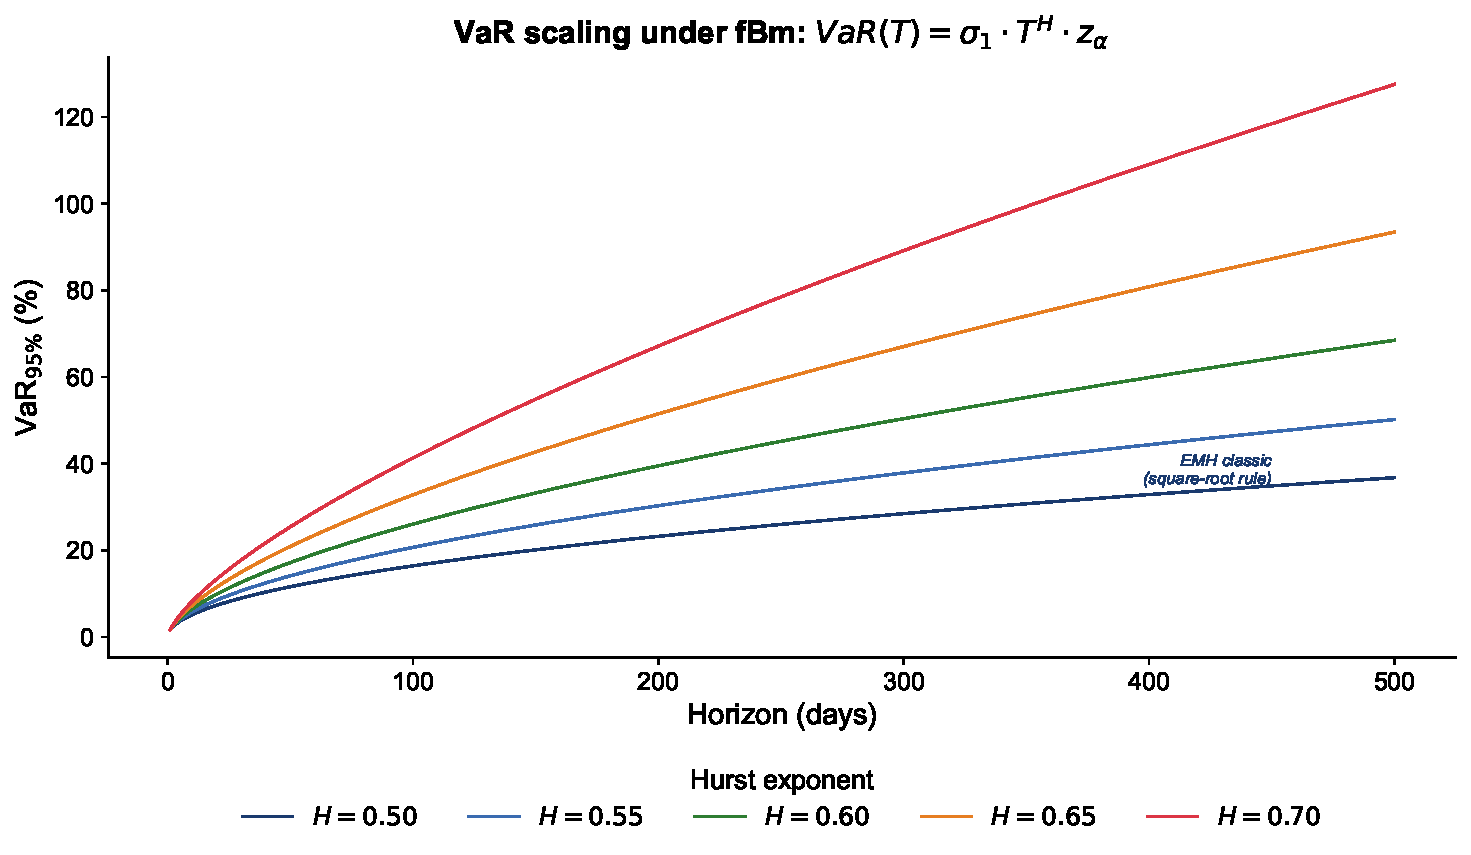
\includegraphics[height=5.4cm,keepaspectratio]{ch_fmh_var_scaling.pdf}\\[2pt]
{\scriptsize\textcolor{MediumGray}{\textit{VaR$_{95\%}$ ca funcție de orizont $T$ pentru valori diferite ale exponentului Hurst. Sub EMH ($H=0.5$, regula $\sqrt{T}$). FMH cu $H>0.5$ produce VaR mai mare pe orizonturi lungi.}}}
\figql{SFM\_ch\_fmh\_extra: var\_scaling}{https://github.com/QuantLet/Stat_fin_markets/tree/master/Quantlets/SFM_ch_fmh}
\end{cminipage}
\end{frame}

\slidelevel{PhD}
\begin{frame}[shrink=15]{FIGARCH și volatilitate cu memorie lungă (long-memory volatility)}
\begin{cminipage}{0.95\textwidth}
\begin{itemize}\setlength{\itemsep}{0pt}
    \item \textbf{FIGARCH} (Fractionally Integrated GARCH, Baillie--Bollerslev--Mikkelsen 1996)
    \item Generalizează GARCH(1,1) cu un \textbf{operator de diferențiere fracționară}:
    \[
        (1 - L)^d \cdot \varepsilon_t^2 = \omega + \beta(L) v_t
    \]
    cu $d \in (0, 1/2)$ pentru memoria lungă a volatilității
    \item Captură: $\Corr(\varepsilon_t^2, \varepsilon_{t-k}^2) \sim k^{2d-1}$ (decadere hiperbolică)
    \item \textbf{Variante extinse}:
    \begin{itemize}\setlength{\itemsep}{0pt}
        \item FIEGARCH (Bollerslev--Mikkelsen 1996): asimetrie + memorie lungă
        \item HYGARCH (Davidson 2004): hyperbolic GARCH
        \item HAR (Heterogeneous Autoregressive, Corsi 2009): cascadă pe orizonturi diferite (1d, 5d, 22d)
    \end{itemize}
    \item HAR este \textbf{conceptual sora FMH}: introduce \textbf{trei orizonturi de investiție} (zilnic, săptămânal, lunar) într-un model GARCH-like
    \item Implementare Python: pachet \texttt{arch} de Sheppard (\texttt{arch\_model(returns, vol='HARCH')})
\end{itemize}
\end{cminipage}
\end{frame}

\slidelevel{PhD}
\begin{frame}[shrink=15]{Pricing-ul opțiunilor sub fBm (Option pricing under fBm)}
\begin{cminipage}{0.95\textwidth}
\begin{itemize}\setlength{\itemsep}{0pt}
    \item \textbf{Probleme cu fBm pur}:
    \begin{itemize}\setlength{\itemsep}{0pt}
        \item fBm nu este \textbf{semimartingală} (Rogers 1997)
        \item $\Rightarrow$ permite \textbf{arbitraj} (Rogers 1997, Cheridito 2003)
        \item Black-Scholes nu se aplică direct
    \end{itemize}
    \item \textbf{Soluții propuse}:
    \begin{itemize}\setlength{\itemsep}{0pt}
        \item \textbf{Mixed fBm} (Cheridito 2001): $X_t = B_t + \rho B^H_t$, este semimartingală pentru $H > 3/4$
        \item \textbf{Wick-Itô integral} (Hu \& Øksendal 2003): permite stochastic calculus modificat
        \item \textbf{Rough volatility models}: Bayer-Friz-Gatheral (2016), volatilitatea $\sim$ fBm cu $H \approx 0{,}1$
    \end{itemize}
    \item \textbf{Rough Heston model} (El Euch \& Rosenbaum 2019):
    \[
        dV_t = \kappa(\theta - V_t) dt + \xi V_t^{1/2} dW^H_t
    \]
    cu $W^H$ fBm de exponent $H \approx 0{,}1$
    \item Captură \textbf{volatility smile} mai bine decât Black-Scholes pe orizonturi scurte
    \item Pachet Python: \texttt{rBergomi} (open source)
\end{itemize}
\end{cminipage}
\end{frame}

% TASK 8: slide nou --- conformal recalibration pentru Hurst și VaR fractal
\slidelevel{PhD}
\begin{frame}[shrink=10]{Conformal recalibration pentru Hurst și VaR fractal (conformal Hurst/VaR)}
\begin{cminipage}{0.95\textwidth}
\begin{block}{Problema}
\begin{itemize}\setlength{\itemsep}{0pt}
    \item $\hat{H}$ are bias și varianță (cf.\ Bias slide); pentru VaR sub fBm, $T^H$ amplifică incertitudinea
\end{itemize}
\end{block}

\begin{alertblock}{Conformal prediction (Vovk et al.\ 2005)}
\begin{itemize}\setlength{\itemsep}{0pt}
    \item Oferă \textbf{coverage finite-sample} valid pentru intervale $\hat{H}$ și VaR/ES
    \item Independent de model parametric --- doar exchangeabilitatea reziduurilor
\end{itemize}
\end{alertblock}

\begin{exampleblock}{Aplicare propusă (Pele, Lessmann, Härdle --- Conformal Oracle, IJF R3)}
\begin{itemize}\setlength{\itemsep}{0pt}
    \item Comparație coverage: parametric vs bootstrap vs conformal
    \item Pe simulări și pe SPY/BTC: conformal menține nominal coverage; bootstrap subestimează
\end{itemize}
\end{exampleblock}
\end{cminipage}
\end{frame}

% TASK 8: slide ML extins (înlocuiește versiunea condensată)
\slidelevel{PhD}
\begin{frame}[shrink=10]{ML și TSFM pentru estimarea Hurst (ML \& TSFM for Hurst)}
\begin{cminipage}{0.95\textwidth}
\begin{block}{Estimatori bazați pe rețele neuronale}
\begin{itemize}\setlength{\itemsep}{0pt}
    \item 1D CNN, LSTM, Transformer pe simulări fBm cu $H$ cunoscut
    \item Han et al.\ (2020), Boudjellaba et al.\ (2022): bate DFA pe MSE
\end{itemize}
\end{block}

\begin{alertblock}{Time-Series Foundation Models (TSFM) pentru regim fractal}
\begin{itemize}\setlength{\itemsep}{0pt}
    \item Chronos-2, TimesFM 2.5, Moirai 2.0 --- detecție regim fractal zero-shot
    \item Vision-Language Models (FINDER framework, research preview) --- crash detection din chart-uri
\end{itemize}
\end{alertblock}

\begin{exampleblock}{Comparație performanță (DGP fBm)}
\begin{itemize}\setlength{\itemsep}{0pt}
    \item Ranking pe MSE estimare $\hat{H}$: TSFM $<$ NN $<$ DFA $<$ R/S clasic
    \item Quantlet: \texttt{SFM\_ch10\_ml\_tsfm\_hurst}
\end{itemize}
\end{exampleblock}
\end{cminipage}
\end{frame}

%#############################################################################
\section{Concluzii și referințe}
%#############################################################################

\slidelevel{Y3}
\begin{frame}[shrink=15]{Concluzii}
\begin{cminipage}{0.95\textwidth}
\begin{itemize}\setlength{\itemsep}{1pt}
    \item \textbf{FMH oferă un cadru mai bogat decât EMH} pentru a înțelege piețele financiare:
    \begin{itemize}\setlength{\itemsep}{0pt}
        \item Piețele sunt stabile când există \textbf{diversitate de orizonturi}
        \item Crah-urile apar când această diversitate se \textbf{prăbușește}
        \item Randamentele prezintă \textbf{autosimilaritate} și \textbf{memorie lungă}, capturate de exponentul Hurst $H$
    \end{itemize}
    \item \textbf{Comparație directă cu EMH}:
    \begin{itemize}\setlength{\itemsep}{0pt}
        \item EMH: $H = 0{,}5$, randamente i.i.d., fără crah-uri dincolo de cozi gaussiene
        \item FMH: $H \neq 0{,}5$, scalare fractală, lichiditate dependentă de orizont, explicație structurală pentru crah-uri
    \end{itemize}
    \item \textbf{Implicații practice}:
    \begin{itemize}\setlength{\itemsep}{0pt}
        \item Modele VaR standard ($H = 0{,}5$) \textbf{subestimează} riscul de coadă
        \item Scalarea volatilității: $\sigma(\Delta) = \sigma(1) \cdot \Delta^H$ în loc de $\Delta^{0{,}5}$
        \item Monitorizarea $\hat{H}_t$ rolling: \textbf{indicator timpuriu} pentru crize de lichiditate
        \item Modele multifractale (MMAR): mai bune predicții de densitate
    \end{itemize}
    \item \textbf{Direcții deschise}: AMH (Lo, 2004), high-frequency fractal, multifractal portfolio, rough volatility (Gatheral et al., 2018)
\end{itemize}
\end{cminipage}
\end{frame}

\slidelevel{MSc}
\begin{frame}[shrink=25]{Referințe principale}
\begin{cminipage}{0.96\textwidth}
\scriptsize
\begin{itemize}\setlength{\itemsep}{1pt}
    \item Bachelier, L. (1900). \textit{Théorie de la spéculation}. Annales Scientifiques de l'École Normale Supérieure.
    \item Hurst, H.E. (1951). Long-term storage capacity of reservoirs. \textit{Trans. ASCE}, 116, 770--808.
    \item Mandelbrot, B.B. (1963). The variation of certain speculative prices. \textit{Journal of Business}, 36(4), 394--419.
    \item Mandelbrot, B.B., Van Ness, J.W. (1968). Fractional Brownian motions, fractional noises and applications. \textit{SIAM Review}, 10(4), 422--437.
    \item Mandelbrot, B.B., Wallis, J.R. (1969). Robustness of the rescaled range R/S in the measurement of noncyclic long run statistical dependence. \textit{Water Resources Research}, 5(5), 967--988.
    \item Mandelbrot, B.B. (1982). \textit{The Fractal Geometry of Nature}. W.H. Freeman.
    \item Peters, E.E. (1991). \textit{Chaos and Order in the Capital Markets}. John Wiley \& Sons.
    \item Peters, E.E. (1994). \textit{Fractal Market Analysis: Applying Chaos Theory to Investment and Economics}. John Wiley \& Sons.
    \item Lo, A.W. (1991). Long-term memory in stock market prices. \textit{Econometrica}, 59(5), 1279--1313.
    \item Peng, C.-K., Buldyrev, S.V., Havlin, S., Simons, M., Stanley, H.E., Goldberger, A.L. (1994). Mosaic organization of DNA nucleotides. \textit{Phys.\ Rev.\ E}, 49(2), 1685--1689.
    \item Mandelbrot, B.B., Fisher, A., Calvet, L. (1997). A multifractal model of asset returns. \textit{Cowles Foundation Discussion Paper} 1164.
    \item Mandelbrot, B.B., Hudson, R.L. (2004). \textit{The (Mis)Behavior of Markets: A Fractal View of Financial Turbulence}. Basic Books.
    \item Lo, A.W. (2004). The adaptive markets hypothesis. \textit{Journal of Portfolio Management}, 30(5), 15--29.
    \item Dominique, C.-R., Rivera-Solis, L.E. (2011). Mixed fractional Brownian motion, short and long-term Dependence and economic conditions: The case of the S\&P 500 Index. \textit{International Business and Management}, 3(2), 1--6.
    \item Gatheral, J., Jaisson, T., Rosenbaum, M. (2018). Volatility is rough. \textit{Quantitative Finance}, 18(6), 933--949.
    \item Pele, D.T., Mazurencu-Marinescu, M. (2014). Modelling stock market volatility using GARCH type models with focus on Romania. \textit{Journal of Applied Quantitative Methods}, 9(1), 1--12.
\end{itemize}
\end{cminipage}
\end{frame}

\slidelevel{MSc}
\begin{frame}[shrink=20]{Comparație finală: EMH vs FMH vs AMH}
\begin{cminipage}{0.95\textwidth}
\renewcommand{\arraystretch}{1.25}
\begin{center}
\scriptsize
\begin{tabular}{llll}
\toprule
\textbf{Aspect} & \textbf{EMH} (1965) & \textbf{FMH} (1991) & \textbf{AMH} (2004) \\
\midrule
Autor principal & Fama & Peters / Mandelbrot & Lo \\
Distribuție rand. & Gaussiană / i.i.d. & Auto-similară (fBm) & Variabilă în timp \\
Hurst & $H = 0{,}5$ & $H \neq 0{,}5$, fix & $H_t$ variabil \\
Memorie & Niciuna & Pe termen lung & Adaptivă \\
Risc primar & Varianța $\sigma^2$ & $H$ + cozi grele & Context-dependent \\
Crah & Lebede negre & Colaps fractal & Ecologic / extincție \\
Investitori & Raționali, identici & Orizonturi diverse & Heuristici evolutive \\
Stabilitate & Mereu echilibru & Diversitate stabilă & Echilibru punctat \\
Predictibilitate & Impredictibil & Fractal patterns & Variabilă în timp \\
Strategii viabile & Doar pasive & Multi-horizon & Adaptive \\
\bottomrule
\end{tabular}
\end{center}
\vspace{0.2cm}
\begin{itemize}\setlength{\itemsep}{0pt}
    \item EMH, FMH, AMH \textbf{nu sunt mutual exclusive}: pot fi văzute ca o ierarhie evolutivă
    \item EMH = condiție limită (lichiditate $\to \infty$, orizonturi $\to$ omogene)
    \item FMH = piețe \textbf{tipice}, cu diversitate finită de orizonturi
    \item AMH = generalizare evoluționistă, captură schimbări structurale
\end{itemize}
\end{cminipage}
\end{frame}

% TASK 3: split slide "Sumarul metodelor" în 2 frame-uri
% TABLE-SLIDE
\slidelevel{Y3}
\begin{frame}[shrink=10]{Sumarul metodelor: tabel (methods summary)}
\begin{cminipage}{0.95\textwidth}
\renewcommand{\arraystretch}{1.25}
\begin{center}
\small
\begin{tabular}{lll}
\toprule
\textbf{Tehnică (technique)} & \textbf{Output} & \textbf{Aplicare} \\
\midrule
Box-counting & Dim. fractală $D$ & Caracterizare obiect \\
R/S analysis & Hurst $\hat{H}$ & Memorie pe termen lung \\
DFA-1, DFA-2, DFA-3 & Hurst $\hat{H}$ (robust) & Trenduri non-staționare \\
MFDFA & Hurst generalizat $h(q)$ & Multifractalitate \\
WTMM (wavelets) & Spectru $\tau(q), f(\alpha)$ & Multifractalitate robustă \\
Variance ratio (Lo--MacKinlay) & Test $H_0: H=0{,}5$ & Random walk testing \\
GPH (semi-parametric) & $\hat{d} \approx \hat{H} - 0{,}5$ & Long memory în frecv. \\
fBm simulation (Davies--Harte) & Traiectorii sintetice & Backtesting, Monte Carlo \\
ARFIMA / FIGARCH & Memorie lungă în randam./vol. & Forecasting volatilitate \\
MSM (Calvet--Fisher) & Multifractal MLE & Forecasting + multifractal \\
\bottomrule
\end{tabular}
\end{center}
\end{cminipage}
\end{frame}

\slidelevel{Y3}
\begin{frame}{Pipeline standard de analiză fractală (standard fractal analysis pipeline)}
\begin{cminipage}{0.95\textwidth}
\begin{block}{Recomandare practică --- 6 pași}
\begin{enumerate}\setlength{\itemsep}{2pt}
    \item \textbf{Vizualizare}: grafic preț + log-randamente
    \item \textbf{Estimare} $\hat{H}$ prin DFA-1 (rapid, robust)
    \item \textbf{Test} $H_0: H = 0{,}5$ prin Variance Ratio
    \item \textbf{Hurst rolling} pentru detecție de regim
    \item \textbf{MFDFA} pentru spectrul multifractal
    \item \textbf{Aplicare} în VaR adjusted, alocare portofoliu, semnal trading
\end{enumerate}
\end{block}
\end{cminipage}
\end{frame}

% TASK 3: redus de la 12 la 5 direcții (cele mai relevante pentru SFM)
\slidelevel{PhD}
\begin{frame}{Direcții deschise de cercetare (open research directions)}
\begin{cminipage}{0.95\textwidth}
\begin{itemize}\setlength{\itemsep}{3pt}
    \item \textbf{Rough volatility} (Gatheral et al.\ 2018): volatilitatea log-realizată este fBm cu $H \approx 0{,}1$ --- \textbf{anti-persistentă}!
    \item \textbf{DeFi}: yield farming, AMM, flash loans introduc noi clase de fractalitate
    \item \textbf{Multifractal portfolio theory}: extinderea Markowitz pentru spectrele $f(\alpha)$
    \item \textbf{Neural ODE pentru fBm}: rețele neuronale care învață direct ecuațiile stocastice fracționare
    \item \textbf{ESG \& fractalitate}: investitorii ESG ca o cohortă cu orizont lung $\Rightarrow$ stabilizatoare?
\end{itemize}
\end{cminipage}
\end{frame}

% TASK 7: glossary acronime
% GLOSSARY-SLIDE
\slidelevel{Y3}
\begin{frame}[shrink=10]{Glossary acronime (acronyms glossary)}
\begin{cminipage}{0.95\textwidth}
\begin{columns}[T]
\begin{column}{0.48\textwidth}
\begin{itemize}\setlength{\itemsep}{0pt}
    \item \textbf{H}: exponentul Hurst
    \item \textbf{$\hat{H}$}: estimator Hurst
    \item \textbf{R/S}: rescaled range
    \item \textbf{DFA}: detrended fluctuation analysis
    \item \textbf{MFDFA}: multifractal DFA
    \item \textbf{fBm}: fractional Brownian motion
    \item \textbf{fGn}: fractional Gaussian noise
    \item \textbf{ARFIMA}: AutoReg. Fractionally Integrated MA
    \item \textbf{FIGARCH}: Fractionally Integrated GARCH
    \item \textbf{MMAR}: Multifractal Model of Asset Returns
\end{itemize}
\end{column}
\begin{column}{0.48\textwidth}
\begin{itemize}\setlength{\itemsep}{0pt}
    \item \textbf{MSM}: Markov-Switching Multifractal
    \item \textbf{GPH}: Geweke--Porter-Hudak
    \item \textbf{WTMM}: Wavelet Transform Modulus Maxima
    \item \textbf{Whittle}: estimator spectral
    \item \textbf{EMH}: Efficient Market Hypothesis
    \item \textbf{FMH}: Fractal Market Hypothesis
    \item \textbf{AMH}: Adaptive Market Hypothesis
    \item \textbf{VaR}: Value-at-Risk
    \item \textbf{ES}: Expected Shortfall
\end{itemize}
\end{column}
\end{columns}
\end{cminipage}
\end{frame}

\slidelevel{Y3}
\begin{frame}[shrink=20]{Mulțumesc!}
\begin{cminipage}{0.92\textwidth}
\begin{center}
{\Large\textcolor{IDAred}{\textbf{Ipoteza Pieței Fractale}}}\\[0.1cm]

\includegraphics[height=2.0cm]{ch_fmh_mandelbrot_full.pdf}\\[1pt]
\figql{SFM\_ch\_fmh\_fractals: mandelbrot\_full}{https://github.com/QuantLet/Stat_fin_markets/tree/master/Quantlets/SFM_ch_fmh}
\end{center}

\vspace{0.05cm}

\begin{alertblock}{Citat de încheiere (Closing quote)}
\begin{itemize}\setlength{\itemsep}{0pt}
    \item \textit{,,Markets are turbulent, deceptive, complex, and fractal.''}\hfill {\scriptsize --- Benoît Mandelbrot}
\end{itemize}
\end{alertblock}

\begin{block}{Contact}
\begin{itemize}\setlength{\itemsep}{0pt}
    \item \scriptsize \textbf{Daniel Traian PELE} --- \texttt{danpele@ase.ro}
    \item \scriptsize \textbf{Antoaneta Amza}
\end{itemize}
\end{block}
\end{cminipage}
\end{frame}

\end{document}
